
\renewcommand{\todo}[1]{}
\newcommand{\notyet}[1]{\footnote{#1 not yet implemented.}}
\newcommand{\Ps}{\mbox{\sl Ps}}
\newcommand{\Ts}{\mbox{\sl Ts}}
\newcommand{\tps}{\mbox{\sl tps}}
\newcommand{\ps}{\mbox{\sl ps}}
\newcommand{\ds}{\mbox{\sl ds}}
\newcommand{\xs}{\mbox{\sl xs}}
\newcommand{\psig}{\mbox{\sl psig}}
\newcommand{\fsig}{\mbox{\sl fsig}}
\newcommand{\csig}{\mbox{\sl csig}}
\newcommand{\args}{\mbox{\sl args}}
\newcommand{\targs}{\mbox{\sl targs}}
\newcommand{\ttcs}{\mbox{\sl ttcs}}
\newcommand{\complx}{\mbox{\sl complexity}}
\newcommand{\enums}{\mbox{\sl enums}}
\newcommand{\proto}{\mbox{\sl pt}}
\newcommand{\argtypes}{\mbox{\sl Ts}}
\newcommand{\stats}{\mbox{\sl stats}}
\newcommand{\overload}{\la\mbox{\sf and}\ra}
\newcommand{\op}{\mbox{\sl op}}

\newcommand{\eqdef}{\stackrel{\mbox{\small eq}}{=}}
\newcommand{\ifqualified}[1]{}
\newcommand{\iflet}[1]{}
\newcommand{\ifundefvar}[1]{}
\newcommand{\iffinaltype}[1]{}
\newcommand{\ifpackaging}[1]{}
\newcommand{\ifnewfor}[1]{}

\newcommand{\U}[1]{\mbox{$\backslash$u{#1}}}
\newcommand{\Urange}[2]{\mbox{$\backslash$u{#1}-$\backslash$u{#2}}}
%\newcommand{\U}[1]{\mbox{U+{#1}}}

\section*{Preface}

% todo: explain constant expressions & types!

Scala is a Java-like programming language which unifies
object-oriented and functional programming.  It is a pure
object-oriented language in the sense that every value is an
object. Types and behavior of objects are described by
classes. Classes can be composed using mixin composition.  Scala is
designed to work seamlessly with two less pure but mainstream
object-oriented languages -- Java and C\#.

Scala is a functional language in the sense that every function is a
value. Nesting of function definitions and higher-order functions are
naturally supported. Scala also supports a general notion of pattern
matching which can model the algebraic types used in many functional
languages.

Scala has been designed to interoperate seamlessly with Java (an
alternative implementation of Scala also works for .NET). Scala
classes can call Java methods, create Java objects, inherit from Java
classes and implement Java interfaces. None of this requires interface
definitions or glue code.

Scala has been developed from 2001 in the programming methods
laboratory at EPFL. Version 1.0 was released in November 2003. This
document describes the second version of the language, which was
released in March 2006. It acts a reference for the language
definition and some core library modules. It is not intended to teach
Scala or its concepts; for this there are other documents 
\cite{scala-overview-tech-report,%
      odersky:scala-experiment,%
      odersky:sca,%
      odersky-et-al:ecoop03,%
      odersky-zenger:fool12}.

Scala has been a collective effort of many people. The design and the
implementation of version 1.0 was completed by Philippe Altherr,
Vincent Cremet, Gilles Dubochet, Burak Emir, St\'ephane Micheloud,
Nikolay Mihaylov, Michel Schinz, Erik Stenman, Matthias Zenger, and
the author. Iulian Dragos, Gilles Dubochet, Philipp Haller, Sean
McDirmid, Lex Spoon, and Geoffrey Washburn joined in the effort to
develop the second version of the language and tools.  Gilad Bracha,
Craig Chambers, Erik Ernst, Matthias Felleisen, Shriram Krishnamurti,
Gary Leavens, Sebastian Maneth, Erik Meijer, Klaus Ostermann, Didier
R\'emy, Mads Torgersen, and Philip Wadler have shaped the design of
the language through lively and inspiring discussions and comments on
previous versions of this document.  The contributors to the Scala
mailing list have also given very useful feedback that helped us
improve the language and its tools.

\chapter{Lexical Syntax}

Scala programs are written using the Unicode Basic Multilingual Plane
(\textsc{bmp}) character set; Unicode supplementary characters are not
presently supported.  This chapter defines the two modes of Scala's
lexical syntax, the Scala mode and the \textsc{xml} mode. If not
otherwise mentioned, the following descriptions of Scala tokens refer
to Scala mode, and literal characters `c' refer to the ASCII fragment
\Urange{0000}{007F}.

In Scala mode, \textit{Unicode escapes} are replaced by the corresponding
Unicode character with the given hexadecimal code.
\begin{lstlisting}
UnicodeEscape ::= \{\\}u{u} hexDigit hexDigit hexDigit hexDigit
hexDigit      ::= `0' | $\cdots$ | `9' | `A' | $\cdots$ | `F' | `a' | $\cdots$ | `f' |
\end{lstlisting}
To construct tokens, characters are distinguished according to the following classes 
(Unicode general category given in parentheses):
\begin{enumerate}
\item Whitespace characters. \U{0020} | \U{0009} | \U{000D} | \U{000A}
\item Letters, which include lower case letters(Ll), upper case letters(Lu), titlecase letters(Lt), other letters(Lo), letter numerals(Nl) and the 
two characters \U{0024} ~\lstinline@`$\Dollar$'@ and \U{005F} ~\lstinline@`_'@, which
both count as upper case letters
\item Digits ~\lstinline@`0' | $\ldots$ | `9'@.
\item Parentheses ~\lstinline@`(' | `)' | `[' | `]' | `{' | `}'@.
\item Delimiter characters ~\lstinline@``' | `'' | `"' | `.' | `;' | `,'@.
\item Operator characters. These consist of all printable ASCII characters \Urange{0020}{007F}. 
which are in none of the sets above, mathematical symbols(Sm) and other symbols(So).
\end{enumerate}
\newpage
\section{Identifiers}\label{sec:idents}

\syntax\begin{lstlisting}
op       ::=  opchar {opchar} 
varid    ::=  lower idrest
plainid  ::=  upper idrest
           |  varid
           |  op
id       ::=  plainid
           |  `\`' stringLit `\`'
idrest   ::=  {letter | digit} [`_' op]
\end{lstlisting}

There are three ways to form an identifier. First, an identifier can
start with a letter which can be followed by an arbitrary sequence of
letters and digits. This may be followed by underscore `\lstinline@_@'
characters and another string composed of either letters and digits or
of operator characters.  Second, an identifier can start with an operator 
character followed by an arbitrary sequence of operator characters.
The preceding two forms are called {\em plain} identifiers.  Finally,
an identifier may also be formed by an arbitrary string between
back-quotes (host systems may impose some restrictions on which
strings are legal for identifiers).  The identifier then is composed
of all characters excluding the backquotes themselves.
 
As usual, a longest match rule applies. For instance, the string

\begin{lstlisting}
big_bob++=`def`
\end{lstlisting}

decomposes into the three identifiers \lstinline@big_bob@, \lstinline@++=@, and
\code{def}.  The rules for pattern matching further distinguish between
{\em variable identifiers}, which start with a lower case letter, and
{\em constant identifiers}, which do not.


The `\lstinline[mathescape=false]@$@'\comment$ character is reserved
for compiler-synthesized identifiers.  User programs should not define
identifiers which contain `\lstinline[mathescape=false]@$@'\comment$
characters.

The following names are reserved words instead of being members of the
syntactic class \code{id} of lexical identifiers.

\begin{lstlisting}
abstract    case        catch       class       def
do          else        extends     false       final
finally     for         forSome     if          implicit
import      lazy        match       new         null
object      override    package     private     protected
return      sealed      super       this        throw       
trait       try         true        type        val         
var         while       with        yield
_    :    =    =>    <-    <:    <%     >:    #    @
\end{lstlisting}

The Unicode operators \U{21D2} `$\Rightarrow$' and \U{2190}
`$\leftarrow$', which have the ASCII equivalents `\lstinline@=>@' and
`\lstinline@<-@', are also reserved.

\example
Here are examples of identifiers:
\begin{lstlisting}
    x         Object        maxIndex   p2p      empty_?
    +         `yield`       $\alpha\rho\epsilon\tau\eta$     _y       dot_product_*
    __system  _MAX_LEN_     
\end{lstlisting}

\example Backquote-enclosed strings are a solution when one needs to
access Java identifiers that are reserved words in Scala. For
instance, the statement ~\lstinline@Thread.yield()@ is illegal, since
\code{yield} is a reserved word in Scala. However, here's a
work-around:
\begin{lstlisting}
Thread.`yield`()
\end{lstlisting}

\section{Newline Characters}\label{sec:newlines}

\syntax\begin{lstlisting}
semi ::= `;' |  nl {nl}
\end{lstlisting}

Scala is a line-oriented language where statements may be terminated by
semi-colons or newlines. A newline in a Scala source text is treated
as the special token ``\lstinline@nl@'' if the three following
criteria are satisfied:
\begin{enumerate}
\item
The token immediately preceding the newline can terminate a statement.
\item
The token immediately following the newline can begin a statement.
\item
The token appears in a region where newlines are enabled.
\end{enumerate}

The tokens that can terminate a statement are: literals, identifiers
and the following delimiters and reserved words:
\begin{lstlisting}
this    null    true    false    return    type    <xml-start>    
_       )       ]       }
\end{lstlisting}

The tokens that can begin a statement are all Scala tokens {\em except}
the following delimiters and reserved words:
\begin{lstlisting}
catch    else    extends    finally    forSome    match        
with    yield    ,    .    ;    :    =    =>    <-    <:    <%    
>:    #    [    )    ]    }
\end{lstlisting}
A \lstinline@case@ token can begin a statement only if followed by a
\lstinline@class@ or \lstinline@object@ token.

Newlines are enabled in:
\begin{enumerate}
\item
all of a Scala source file, except for nested regions where newlines
are disabled, and
\item
the interval between matching \lstinline@{@ and \lstinline@}@ brace tokens,
except for nested regions where newlines are disabled.
\end{enumerate}

Newlines are disabled in:
\begin{enumerate}
\item
the interval between matching \lstinline@(@ and \lstinline@)@ parenthesis tokens, except for nested regions where newlines are enabled, and
\item
the interval between matching \lstinline@[@ and \lstinline@]@ bracket tokens,
except for nested regions where newlines are enabled.
\item
The interval between a \lstinline@case@ token and its matching
\lstinline@=>@ token, except for nested regions where newlines are
enabled.
\item Any regions analyzed in XML mode (\sref{sec::xmlMode}).
\end{enumerate}
Note that the brace characters of \lstinline@{...}@ escapes in XML and
string literals are not tokens, 
and therefore do not enclose a region where newlines
are enabled.

Normally, only a single \code{nl} token is inserted between two
consecutive non-newline tokens which are on different lines, even if there are multiple lines
between the two tokens. However, if two tokens are separated by at
least one completely blank line (i.e a line which contains no
printable characters), then two \code{nl} tokens are inserted.

The Scala grammar (given in full in Appendix~\ref{sec:syntax})
contains productions where optional \code{nl} tokens, but not
semicolons, are accepted. This has the effect that a newline in one of these
positions does not terminate an expression or statement. These positions can
be summarized as follows:

Multiple newline tokens are accepted in the following places (note
that a semicolon in place of the newline would be illegal in every one
of these cases):
\begin{itemize}
\item[--]
between the condition of an conditional expression
(\sref{sec:cond}) or while loop (\sref{sec:while}) and the next
following expression,
\item[--]
between the enumerators of a for-comprehension (\sref{sec:for-comprehensions})
and the next following expression, and
\item[--]
after the initial \lstinline@type@ keyword in a type definition or
declaration (\sref{sec:typedcl}).
\end{itemize}
A single new line token is accepted
\begin{itemize}
\item[--] 
  in front of an opening brace ``$\{$'', if that brace is a legal
  continuation of the current statement or expression,
\item[--]
  after an infix operator, if the first token on the next line can
  start an expression (\sref{sec:infix-operations}),
\item[--]
  in front of a parameter clause (\sref{sec:funsigs}), and
\item[--]
  after an annotation (\sref{sec:annotations}).
\end{itemize}  

\example The following code contains four well-formed statements, each
on two lines. The newline tokens between the two lines are not
treated as statement separators.
\begin{lstlisting}
if (x > 0)
  x = x - 1

while (x > 0)
  x  = x / 2

for (x <- 1 to 10)
  println(x)

type
  IntList = List[Int]
\end{lstlisting}

\example The following code designates an anonymous class
\begin{lstlisting}
new Iterator[Int]
{
  private var x = 0
  def hasNext = true
  def next = { x += 1; x }
}
\end{lstlisting}

With an additional newline character, the same code is interpreted as
an object creation followed by a local block:

\begin{lstlisting}
new Iterator[Int] 

{
  private var x = 0
  def hasNext = true
  def next = { x += 1; x }
}
\end{lstlisting}

\example The following code designates a single expression:

\begin{lstlisting}
  x < 0 ||
  x > 10
\end{lstlisting}

With an additional newline character, the same code is interpreted as
two expressions:

\begin{lstlisting}
  x < 0 ||

  x > 10
\end{lstlisting}

\example The following code designates a single, curried function definition:

\begin{lstlisting}
  def func(x: Int)
          (y: Int) = x + y
\end{lstlisting}

With an additional newline character, the same code is interpreted as
an abstract function definition and a syntactically illegal statement:

\begin{lstlisting}
  def func(x: Int)

          (y: Int) = x + y
\end{lstlisting}

\example The following code designates an attributed definition:

\begin{lstlisting}
  @serializable
  protected class Data { ... }
\end{lstlisting}

With an additional newline character, the same code is interpreted as
an attribute and a separate statement (which is syntactically
illegal).

\begin{lstlisting}
  @serializable

  protected class Data { ... }
\end{lstlisting}


\section{Literals}\label{sec:literals}

There are literals for integer numbers, floating point numbers,
characters, booleans, symbols, strings.  The syntax of these literals is in
each case as in Java.

\todo{say that we take values from Java, give examples of some lits in
  particular float and double.}

\syntax\begin{lstlisting}
Literal  ::=  [`-'] integerLiteral
           |  [`-'] floatingPointLiteral
           |  booleanLiteral
           |  characterLiteral
           |  stringLiteral
           |  symbolLiteral
           |  `null'
\end{lstlisting}

\subsection{Integer Literals}

\syntax\begin{lstlisting}
integerLiteral  ::=  (decimalNumeral | hexNumeral) [`L' | `l']
decimalNumeral  ::=  `0' | nonZeroDigit {digit}
hexNumeral      ::=  `0' `x' hexDigit {hexDigit}
digit           ::=  `0' | nonZeroDigit
nonZeroDigit    ::=  `1' | $\cdots$ | `9'
\end{lstlisting}
Integer literals are usually of type \lstinline@Int@, or of type
\lstinline@Long@ when followed by a \lstinline@L@ or
\lstinline@l@ suffix. Values of type \lstinline@Int@ are all integer
numbers between $-2^{31}$ and $2^{31}-1$, inclusive.  Values of
type \lstinline@Long@ are all integer numbers between $-2^{63}$ and
$2^{63}-1$, inclusive. A compile-time error occurs if an integer literal
denotes a number outside these ranges.

However, if the expected type $\proto$ (\sref{sec:expr-typing}) of a literal
in an expression is either \code{Byte}, \code{Short}, or \code{Char}
and the integer number fits in the numeric range defined by the type,
then the number is converted to type $\proto$ and the literal's type
is $\proto$. The numeric ranges given by these types are:
\begin{quote}
\begin{tabular}{p{2cm}{l}}
\lstinline@Byte@ & $-2^7$ to $2^7-1$ \\
\lstinline@Short@ & $-2^{15}$ to $2^{15}-1$ \\
\lstinline@Char@ & $0$ to $2^{16}-1$
\end{tabular}
\end{quote}

\example
Here are some integer literals:
\begin{lstlisting}
0          21          0xFFFFFFFF       -42L
\end{lstlisting}

\subsection{Floating Point Literals}

\syntax\begin{lstlisting}
floatingPointLiteral  ::=  digit {digit} `.' {digit} [exponentPart] [floatType]
                        |  `.' digit {digit} [exponentPart] [floatType]
                        |  digit {digit} exponentPart [floatType]
                        |  digit {digit} [exponentPart] floatType
exponentPart          ::=  (`E' | `e') [`+' | `-'] digit {digit}
floatType             ::=  `F' | `f' | `D' | `d'
\end{lstlisting}
Floating point literals are of type \lstinline@Float@ when followed by
a floating point type suffix \lstinline@F@ or \lstinline@f@, and are
of type \lstinline@Double@ otherwise.  The type \lstinline@Float@
consists of all IEEE 754 32-bit single-precision binary floating point
values, whereas the type \lstinline@Double@ consists of all IEEE 754
64-bit double-precision binary floating point values.

If a floating point literal in a program is followed by a token
starting with a letter, there must be at least one intervening
whitespace character between the two tokens.

\example
Here are some floating point literals:
\begin{lstlisting}
0.0        1e30f      3.14159f      1.0e-100      .1
\end{lstlisting}

\example
The phrase `\lstinline@1.toString@' parses as three different tokens:
`\lstinline@1@', `\lstinline@.@', and `\lstinline@toString@'. On the
other hand, if a space is inserted after the period, the phrase
`\lstinline@1. toString@' parses as the floating point literal
`\lstinline@1.@' followed by the identifier `\lstinline@toString@'.






\subsection{Boolean Literals}

\syntax\begin{lstlisting}
booleanLiteral  ::=  `true' | `false'
\end{lstlisting}

The boolean literals \lstinline@true@ and \lstinline@false@ are
members of type \lstinline@Boolean@.

\subsection{Character Literals}

\syntax\begin{lstlisting}
characterLiteral  ::=  `\'' printableChar `\''
                    |  `\'' charEscapeSeq `\''
\end{lstlisting}

A character literal is a single character enclosed in quotes.
The character is either a printable unicode character or is described
by an escape sequence (\sref{sec:escapes}).

\example
Here are some character literals:
\begin{lstlisting}
'a'    '\u0041'    '\n'    '\t'
\end{lstlisting}
Note that `\lstinline@\u000A@' is {\em not} a valid character literal because
Unicode conversion is done before literal parsing and the Unicode
character \lstinline@\u000A@ (line feed) is not a printable
character. One can use instead the escape sequence `\lstinline@\n@' or
the octal escape `\lstinline@\12@' (\sref{sec:escapes}).

\subsection{String Literals}\label{sec:string-literals}

\syntax\begin{lstlisting}
stringLiteral  ::=  `\"' {stringElement} `\"'
stringElement  ::=  printableCharNoDoubleQuote  |  charEscapeSeq
\end{lstlisting}

A string literal is a sequence of characters in double quotes.  The
characters are either printable unicode character or are described by
escape sequences (\sref{sec:escapes}). If the string literal
contains a double quote character, it must be escaped,
i.e.\ \lstinline@\"@. The value of a string literal is an instance of
class \lstinline@String@. 

\example
Here are some string literals:
\begin{lstlisting}
"Hello,\nWorld!"       
"This string contains a \" character."
\end{lstlisting}

\subsubsection*{Multi-Line String Literals}

\syntax\begin{lstlisting}
stringLiteral   ::=  `"""' multiLineChars `"""'
multiLineChars  ::=  {['"'] ['"'] charNoDoubleQuote} {`"'}
\end{lstlisting}

A multi-line string literal is a sequence of characters enclosed in
triple quotes ~\lstinline@""" ... """@. The sequence of characters is
arbitrary, except that it may contain three or more consuctive quote characters
only at the very end. Characters
must not necessarily be printable; newlines or other
control characters are also permitted.  Unicode escapes work as everywhere else, but none
of the escape sequences in (\sref{sec:escapes}) is interpreted.

\example Here is a multi-line string literal:
\begin{lstlisting}
  """the present string
     spans three 
     lines."""
\end{lstlisting}
This would produce the string:
\begin{lstlisting}
the present string
     spans three 
     lines.
\end{lstlisting}
The Scala library contains a utility method \lstinline@stripMargin@
which can be used to strip leading whitespace from multi-line strings.
The expression
\begin{lstlisting}
 """the present string
   |spans three 
   |lines.""".stripMargin
\end{lstlisting}
evaluates to
\begin{lstlisting}
the present string
spans three 
lines.
\end{lstlisting}
Method \lstinline@stripMargin@ is defined in class
\lstinline@scala.collection.immutable.StringLike@. 
Because there is a predefined
implicit conversion (\sref{sec:impl-conv}) from \code{String} to
\code{StringLike}, the method is applicable to all strings.

\subsection{Escape Sequences}\label{sec:escapes}

The following escape sequences are recognized in character and string
literals.
\begin{quote}
\begin{tabular}{p{2cm}ll}
\lstinline@\b@ & \lstinline@\u0008@: backspace BS \\
\lstinline@\t@ & \lstinline@\u0009@: horizontal tab HT \\
\lstinline@\n@ & \lstinline@\u000a@: linefeed LF \\
\lstinline@\f@ & \lstinline@\u000c@: form feed FF\\
\lstinline@\r@ & \lstinline@\u000d@: carriage return CR\\
\lstinline@\"@ & \lstinline@\u0022@: double quote "\\
\lstinline@\'@ & \lstinline@\u0027@: single quote '\\
\lstinline@\\@ & \lstinline@\u005c@: backslash \lstinline@\@\\
\end{tabular}
\end{quote}
A character with Unicode between 0 and 255 may also be represented by
an octal escape, i.e.\ a backslash `\lstinline@\@' followed by a
sequence of up to three octal characters.

It is a compile time error if a backslash character in a character or
string literal does not start a valid escape sequence.

\subsection{Symbol literals}

\syntax\begin{lstlisting}
symbolLiteral  ::=  `'' plainid
\end{lstlisting}

A symbol literal ~\lstinline@'$x$@~ is a shorthand for the expression
~\lstinline@scala.Symbol("$x$")@. \lstinline@Symbol@ is a case class
(\sref{sec:case-classes}), which is defined as follows.
\begin{lstlisting}
package scala
final case class Symbol private (name: String) {
  override def toString: String = "'" + name
}
\end{lstlisting}
The \lstinline@apply@ method of \lstinline@Symbol@'s companion object
caches weak references to \lstinline@Symbol@s, thus ensuring that
identical symbol literals are equivalent with respect to reference
equality.

\section{Whitespace and Comments}

Tokens may be separated by whitespace characters
and/or comments. Comments come in two forms:

A single-line comment is a sequence of characters which starts with
\lstinline@//@ and extends to the end of the line.

A multi-line comment is a sequence of characters between
\lstinline@/*@ and \lstinline@*/@. Multi-line comments may be nested,
but are required to be properly nested.  Therefore, a comment like
\lstinline@/* /* */@ will be rejected as having an unterminated
comment.

\section{XML mode\label{sec::xmlMode}}

In order to allow literal inclusion of XML fragments, lexical analysis
switches from Scala mode to XML mode when encountering an opening
angle bracket '<' in the following circumstance: The '<' must be
preceded either by whitespace, an opening parenthesis or an opening
brace and immediately followed by a character starting an XML name.

\syntax\begin{lstlisting}
 ( whitespace | `(' | `{' ) `<' (XNameStart | `!' | `?')

  XNameStart ::= `_' | BaseChar | Ideographic $\mbox{\rm\em (as in W3C XML, but without }$ `:'
\end{lstlisting}

The scanner switches from XML mode to Scala mode if either
\begin{itemize}
\item the XML expression or the XML pattern started by the initial '<' has been 
successfully parsed, or if

\item the parser encounters an embedded Scala expression or pattern and 
forces the Scanner 
back to normal mode, until the Scala expression or pattern is
successfully parsed. In this case, since code and XML fragments can be
nested, the parser has to maintain a stack that reflects the nesting
of XML and Scala expressions adequately.
\end{itemize}

Note that no Scala tokens are constructed in XML mode, and that comments are interpreted
as text.

\example 
The following value definition uses an XML literal with two embedded
Scala expressions
\begin{lstlisting}
val b = <book>
          <title>The Scala Language Specification</title>
          <version>{scalaBook.version}</version>
          <authors>{scalaBook.authors.mkList("", ", ", "")}</authors>
        </book>
\end{lstlisting}

\chapter{\label{sec:names}Identifiers, Names and Scopes}

Names in Scala identify types, values, methods, and classes which are
collectively called {\em entities}. Names are introduced by local
definitions and declarations (\sref{sec:defs}), inheritance (\sref{sec:members}),
import clauses (\sref{sec:import}), or package clauses
(\sref{sec:packagings}) which are collectively called {\em
bindings}.

Bindings of different kinds have a precedence defined on them:
\begin{enumerate} 
\item Definitions and declarations that are local, inherited, or made 
available by a package clause in the same compilation unit where the 
definition occurs have highest precedence. 
\item Explicit imports have next highest precedence.
\item Wildcard imports  have next highest precedence.
\item Definitions made available by a package clause not in the 
compilation unit where the definition occurs have lowest precedence.
\end{enumerate} 

There are two different name spaces, one for types (\sref{sec:types})
and one for terms (\sref{sec:exprs}).  The same name may designate a
type and a term, depending on the context where the name is used.

A binding has a {\em scope} in which the entity defined by a single
name can be accessed using a simple name. Scopes are nested.  A binding
in some inner scope {\em shadows} bindings of lower precedence in the
same scope as well as bindings of the same or lower precedence in outer
scopes. 

Note that shadowing is only a partial order. In a situation like
\begin{lstlisting}
val x = 1;
{ import p.x; 
  x }
\end{lstlisting}
neither binding of \code{x} shadows the other. Consequently, the
reference to \code{x} in the third line above would be ambiguous.

A reference to an unqualified (type- or term-) identifier $x$ is bound
by the unique binding, which
\begin{itemize}
\item defines an entity with name $x$ in the same namespace as the
identifier, and
\item shadows all other bindings that define entities with name $x$ in that namespace.
\end{itemize}
It is an error if no such binding exists.  If $x$ is bound by an
import clause, then the simple name $x$ is taken to be equivalent to
the qualified name to which $x$ is mapped by the import clause. If $x$
is bound by a definition or declaration, then $x$ refers to the entity
introduced by that binding. In that case, the type of $x$ is the type
of the referenced entity.

\example Assume the following two definitions of a objects named \lstinline@X@ in packages \lstinline@P@ and \lstinline@Q@.
%ref: shadowing.scala
\begin{lstlisting}
package P {
  object X { val x = 1; val y = 2 }
}
\end{lstlisting}
\begin{lstlisting}
package Q {
  object X { val x = true; val y = "" }
}
\end{lstlisting}
The following program illustrates different kinds of bindings and
precedences between them.
\begin{lstlisting}
package P {                  // `X' bound by package clause
import Console._             // `println' bound by wildcard import
object A {                   
  println("L4: "+X)          // `X' refers to `P.X' here
  object B {
    import Q._               // `X' bound by wildcard import
    println("L7: "+X)        // `X' refers to `Q.X' here
    import X._               // `x' and `y' bound by wildcard import
    println("L8: "+x)        // `x' refers to `Q.X.x' here
    object C {
      val x = 3              // `x' bound by local definition
      println("L12: "+x)     // `x' refers to constant `3' here
      { import Q.X._         // `x' and `y' bound by wildcard import
//      println("L14: "+x)   // reference to `x' is ambiguous here
        import X.y           // `y' bound by explicit import
        println("L16: "+y)   // `y' refers to `Q.X.y' here
        { val x = "abc"      // `x' bound by local definition
          import P.X._       // `x' and `y' bound by wildcard import
//        println("L19: "+y) // reference to `y' is ambiguous here
          println("L20: "+x) // `x' refers to string ``abc'' here
}}}}}}
\end{lstlisting}

A reference to a qualified (type- or term-) identifier $e.x$ refers to
the member of the type $T$ of $e$ which has the name $x$ in the same
namespace as the identifier. It is an error if $T$ is not a value type
(\sref{sec:value-types}). The type of $e.x$ is the member type of the
referenced entity in $T$.

\chapter{\label{sec:types}Types}

\syntax\begin{lstlisting}
  Type              ::=  FunctionArgTypes `=>' Type
                      |  InfixType [ExistentialClause]
  FunctionArgTypes  ::= InfixType
                      | `(' [ ParamType {`,' ParamType } ] `)'
  ExistentialClause ::=  `forSome' `{' ExistentialDcl {semi ExistentialDcl} `}'
  ExistentialDcl    ::=  `type' TypeDcl 
                      |  `val' ValDcl
  InfixType         ::=  CompoundType {id [nl] CompoundType}
  CompoundType      ::=  AnnotType {`with' AnnotType} [Refinement]
                      |  Refinement
  AnnotType         ::=  SimpleType {Annotation}
  SimpleType        ::=  SimpleType TypeArgs
                      |  SimpleType `#' id
                      |  StableId
                      |  Path `.' `type'
                      |  `(' Types ')'
  TypeArgs          ::=  `[' Types `]'
  Types             ::=  Type {`,' Type}
\end{lstlisting}

We distinguish between first-order types and type constructors, which
take type parameters and yield types. A subset of first-order types
called {\em value types} represents sets of (first-class) values.
Value types are either {\em concrete} or {\em abstract}. 

Every concrete value type can be represented as a {\em class type}, i.e.\ a
type designator (\sref{sec:type-desig}) that refers to a
a class or a trait\footnote{We assume that objects and packages also implicitly
define a class (of the same name as the object or package, but
inaccessible to user programs).} (\sref{sec:class-defs}), or as a {\em
compound type} (\sref{sec:compound-types}) representing an
intersection of types, possibly with a refinement
(\sref{sec:refinements}) that further constrains the types of its
members.
\comment{A shorthand exists for denoting function types (\sref{sec:function-types}).  }
Abstract value types are introduced by type parameters (\sref{sec:type-params}) 
and abstract type bindings (\sref{sec:typedcl}). Parentheses in types can be used for
grouping.

%@M
Non-value types capture properties of identifiers that are not values
(\sref{sec:synthetic-types}). For example, a type constructor (\sref{sec:higherkinded-types}) does not directly specify a type of values. However, when a type constructor is applied to the correct type arguments, it yields a first-order type, which may be a value type. 

Non-value types are expressed indirectly in Scala. E.g., a method type is described by writing down a method signature, which in itself is not a real type, although it  gives rise to a corresponding method type (\sref{sec:method-types}). Type constructors are another example, as one can write \lstinline@type Swap[m[_, _], a,b] = m[b, a]@, but there is no syntax to write the corresponding anonymous type function directly.

\section{Paths}\label{sec:paths}\label{sec:stable-ids}

\syntax\begin{lstlisting}
  Path            ::=  StableId
                    |  [id `.'] this
  StableId        ::=  id
                    |  Path `.' id
                    |  [id '.'] `super' [ClassQualifier] `.' id
  ClassQualifier  ::= `[' id `]'
\end{lstlisting}

Paths are not types themselves, but they can be a part of named types
and in that function form a central role in Scala's type system.

A path is one of the following.
\begin{itemize}
\item
The empty path $\epsilon$ (which cannot be written explicitly in user programs).
\item
\lstinline@$C$.this@, where $C$ references a class. 
The path \code{this} is taken as a shorthand for \lstinline@$C$.this@ where 
$C$ is the name of the class directly enclosing the reference. 
\item
\lstinline@$p$.$x$@ where $p$ is a path and $x$ is a stable member of $p$.
{\em Stable members} are packages or members introduced by object definitions or 
by value definitions of non-volatile types
(\sref{sec:volatile-types}). 

\item
\lstinline@$C$.super.$x$@ or \lstinline@$C$.super[$M\,$].$x$@
where $C$ references a class and $x$ references a 
stable member of the super class or designated parent class $M$ of $C$. 
The prefix \code{super} is taken as a shorthand for \lstinline@$C$.super@ where 
$C$ is the name of the class directly enclosing the reference. 
\end{itemize}
A {\em stable identifier} is a path which ends in an identifier.

\section{Value Types}\label{sec:value-types}

Every value in Scala has a type which is of one of the following
forms.

\subsection{Singleton Types}
\label{sec:singleton-types}
\label{sec:type-stability}

\syntax\begin{lstlisting}
  SimpleType  ::=  Path `.' type
\end{lstlisting}

A singleton type is of the form \lstinline@$p$.type@, where $p$ is a
path pointing to a value expected to conform (\sref{sec:expr-typing})
to \lstinline@scala.AnyRef@.  The type denotes the set of values
consisting of \code{null} and the value denoted by $p$. 

A {\em stable type} is either a singleton type or a type which is
declared to be a subtype of trait \lstinline@scala.Singleton@.

\subsection{Type Projection}
\label{sec:type-project}

\syntax\begin{lstlisting} 
  SimpleType  ::=  SimpleType `#' id
\end{lstlisting}

A type projection \lstinline@$T$#$x$@ references the type member named
$x$ of type $T$. 
% The following is no longer necessary:
%If $x$ references an abstract type member, then $T$ must be a stable type (\sref{sec:singleton-types}). 

\subsection{Type Designators}
\label{sec:type-desig}

\syntax\begin{lstlisting}
  SimpleType  ::=  StableId
\end{lstlisting}

A type designator refers to a named value type. It can be simple or
qualified. All such type designators are shorthands for type projections.

Specifically, the unqualified type name $t$ where $t$ is bound in some
class, object, or package $C$ is taken as a shorthand for
\lstinline@$C$.this.type#$t$@. If $t$ is
not bound in a class, object, or package, then $t$ is taken as a
shorthand for \lstinline@$\epsilon$.type#$t$@.

A qualified type designator has the form \lstinline@$p$.$t$@ where $p$ is
a path (\sref{sec:paths}) and $t$ is a type name. Such a type designator is
equivalent to the type projection \lstinline@$p$.type#$t$@.

\example 
Some type designators and their expansions are listed below. We assume
a local type parameter $t$, a value \code{maintable}
with a type member \code{Node} and the standard class \lstinline@scala.Int@, 
\begin{lstlisting}
  t                     $\epsilon$.type#t
  Int                   scala.type#Int
  scala.Int             scala.type#Int
  data.maintable.Node   data.maintable.type#Node
\end{lstlisting}

\subsection{Parameterized Types}
\label{sec:param-types}

\syntax\begin{lstlisting}
  SimpleType      ::=  SimpleType TypeArgs
  TypeArgs        ::=  `[' Types `]'
\end{lstlisting}

A parameterized type $T[U_1 \commadots U_n]$ consists of a type
designator $T$ and type parameters $U_1 \commadots U_n$ where $n \geq
1$.  $T$ must refer to a type constructor which takes $n$ type
parameters $a_1 \commadots a_n$.

Say the type parameters have lower bounds $L_1 \commadots L_n$ and
upper bounds $U_1 \commadots U_n$.  The parameterized type is
well-formed if each actual type parameter {\em conforms to its
bounds}, i.e.\ $\sigma L_i <: T_i <: \sigma U_i$ where $\sigma$ is the
substitution $[a_1 := T_1 \commadots a_n := T_n]$.

\example\label{ex:param-types}
Given the partial type definitions:

\begin{lstlisting}
  class TreeMap[A <: Comparable[A], B] { $\ldots$ }
  class List[A] { $\ldots$ }
  class I extends Comparable[I] { $\ldots$ }
  
  class F[M[_], X] { $\ldots$ }
  class S[K <: String] { $\ldots$ }
  class G[M[ Z <: I ], I] { $\ldots$ }
\end{lstlisting}

the following parameterized types are well formed:

\begin{lstlisting}
  TreeMap[I, String]
  List[I]
  List[List[Boolean]]
  
  F[List, Int]
  G[S, String]
\end{lstlisting}

\example Given the type definitions of \ref{ex:param-types},
the following types are ill-formed:

\begin{lstlisting}
  TreeMap[I]            // illegal: wrong number of parameters
  TreeMap[List[I], Int] // illegal: type parameter not within bound
  
  F[Int, Boolean]       // illegal: Int is not a type constructor
  F[TreeMap, Int]       // illegal: TreeMap takes two parameters,
                        //   F expects a constructor taking one
  G[S, Int]             // illegal: S constrains its parameter to
                        //   conform to String,
                        // G expects type constructor with a parameter
                        //   that conforms to Int
\end{lstlisting}

\subsection{Tuple Types}\label{sec:tuple-types}

\syntax\begin{lstlisting}
  SimpleType    ::=   `(' Types ')'
\end{lstlisting}

A tuple type \lstinline@($T_1 \commadots T_n$)@ is an alias for the
class ~\lstinline@scala.Tuple$n$[$T_1 \commadots T_n$]@, where $n \geq
2$.

Tuple classes are case classes whose fields can be accessed using
selectors ~\code{_1}, ..., \lstinline@_$n$@. Their functionality is
abstracted in a corresponding \code{Product} trait. The $n$-ary tuple
class and product trait are defined at least as follows in the
standard Scala library (they might also add other methods and
implement other traits).

\begin{lstlisting}
case class Tuple$n$[+T1, ..., +T$n$](_1: T1, ..., _$n$: T$n$) 
extends Product$n$[T1, ..., T$n$]

trait Product$n$[+T1, +T2, +T$n$] {
  override def productArity = $n$
  def _1: T1
  ...
  def _$n$:T$n$
}
\end{lstlisting}

\subsection{Annotated Types}

\syntax\begin{lstlisting}
  AnnotType  ::=  SimpleType {Annotation}
\end{lstlisting}

An annotated type ~$T$\lstinline@ $a_1 \ldots a_n$@
attaches annotations $a_1 \commadots a_n$ to the type $T$
(\sref{sec:annotations}).

\example The following type adds the \code{@suspendable}@ annotation to the type
\code{String}:
\begin{lstlisting}
  String @suspendable
\end{lstlisting}

\subsection{Compound Types}
\label{sec:compound-types}
\label{sec:refinements}

\syntax\begin{lstlisting}
  CompoundType    ::=  AnnotType {`with' AnnotType} [Refinement]
                    |  Refinement
  Refinement      ::=  [nl] `{' RefineStat {semi RefineStat} `}'
  RefineStat      ::=  Dcl
                    |  `type' TypeDef
                    |
\end{lstlisting}

A compound type ~\lstinline@$T_1$ with $\ldots$ with $T_n$ {$R\,$}@~
represents objects with members as given in the component types $T_1
\commadots T_n$ and the refinement \lstinline@{$R\,$}@. A refinement
\lstinline@{$R\,$}@ contains declarations and type definitions. 
If a declaration or definition overrides a declaration or definition in
one of the component types $T_1 \commadots T_n$, the usual rules for
overriding (\sref{sec:overriding}) apply; otherwise the declaration
or definition is said to be ``structural''\footnote{A reference to a
structurally defined member (method call or access to a value or
variable) may generate binary code that is significantly slower than
an equivalent code to a non-structural member.}. 

Within a method declaration in a structural refinement, the type of
any value parameter may only refer to type parameters or abstract
types that are contained inside the refinement. That is, it must refer
either to a type parameter of the method itself, or to a type
definition within the refinement. This restriction does not apply to
the function's result type.

If no refinement is given, the empty refinement is implicitly added,
i.e.\  ~\lstinline@$T_1$ with $\ldots$ with $T_n$@~ is a shorthand for
~\lstinline@$T_1$ with $\ldots$ with $T_n$ {}@.

A compound type may also consist of just a refinement
~\lstinline@{$R\,$}@ with no preceding component types. Such a type is
equivalent to ~\lstinline@AnyRef{$R\,$}@.

\example The following example shows how to declare and use a function which parameter's type contains a refinement with structural declarations.
\begin{lstlisting}[escapechar=\%]
  case class Bird (val name: String) extends Object {
  	def fly(height: Int) = ...
	...
  }
  case class Plane (val callsign: String) extends Object {
  	def fly(height: Int) = ...
	...
  }
  def takeoff(
  	    runway: Int,
        r: { val callsign: String; def fly(height: Int) }) = {
    tower.print(r.callsign + " requests take-off on runway " + runway)
    tower.read(r.callsign + " is clear f%%or take-off")
    r.fly(1000)
  }
  val bird = new Bird("Polly the parrot"){ val callsign = name }
  val a380 = new Plane("TZ-987")
  takeoff(42, bird)
  takeoff(89, a380)
\end{lstlisting}
Although ~\lstinline@Bird@ and ~\lstinline@Plane@ do not share any parent class other than ~\lstinline@Object@, the parameter ~\lstinline@r@ of function ~\lstinline@takeoff@ is defined using a refinement with structural declarations to accept any object that declares a value ~\lstinline@callsign@ and a ~\lstinline@fly@ function.

 
\subsection{Infix Types}\label{sec:infix-types}

\syntax\begin{lstlisting}
  InfixType     ::=  CompoundType {id [nl] CompoundType}
\end{lstlisting}
An infix type ~\lstinline@$T_1\;\op\;T_2$@~ consists of an infix
operator $\op$ which gets applied to two type operands $T_1$ and
$T_2$.  The type is equivalent to the type application $\op[T_1,
T_2]$.  The infix operator $\op$ may be an arbitrary identifier,
except for \code{*}, which is reserved as a postfix modifier 
denoting a repeated parameter type (\sref{sec:repeated-params}). 

All type infix operators have the same precedence; parentheses have to
be used for grouping. The associativity (\sref{sec:infix-operations})
of a type operator is determined as for term operators: type operators
ending in a colon `\lstinline@:@' are right-associative; all other
operators are left-associative.

In a sequence of consecutive type infix operations $t_0; \op_1; t_1;
\op_2 \ldots \op_n; t_n$, all operators $\op_1 \commadots \op_n$ must have the same
associativity. If they are all left-associative, the sequence is
interpreted as $(\ldots(t_0;\op_1;t_1);\op_2\ldots);\op_n;t_n$,
otherwise it is interpreted as $t_0;\op_1;(t_1;\op_2;(\ldots\op_n;t_n)\ldots)$.

\subsection{Function Types}
\label{sec:function-types}

\syntax\begin{lstlisting}
  Type              ::=  FunctionArgs `=>' Type
  FunctionArgs      ::=  InfixType
                      |  `(' [ ParamType {`,' ParamType } ] `)'
\end{lstlisting}
The type ~\lstinline@($T_1 \commadots T_n$) => $U$@~ represents the set of function
values that take arguments of types $T_1 \commadots T_n$ and yield
results of type $U$.  In the case of exactly one argument type
~\lstinline@$T$ => $U$@~ is a shorthand for ~\lstinline@($T\,$) => $U$@.  
An argument type of the form~\lstinline@=> T@
represents a call-by-name parameter (\sref{sec:by-name-params}) of type $T$.

Function types associate to the right, e.g.
~\lstinline@$S$ => $T$ => $U$@~ is the same as 
~\lstinline@$S$ => ($T$ => $U$)@.

Function types are shorthands for class types that define \code{apply}
functions.  Specifically, the $n$-ary function type 
~\lstinline@($T_1 \commadots T_n$) => U@~ is a shorthand for the class type
\lstinline@Function$n$[$T_1 \commadots T_n$,$U\,$]@. Such class
types are defined in the Scala library for $n$ between 0 and 9 as follows.
\begin{lstlisting}
package scala 
trait Function$n$[-$T_1 \commadots$ -$T_n$, +$R$] {
  def apply($x_1$: $T_1 \commadots x_n$: $T_n$): $R$ 
  override def toString = "<function>" 
}
\end{lstlisting}
Hence, function types are covariant (\sref{sec:variances}) in their
result type and contravariant in their argument types.


\subsection{Existential Types}
\label{sec:existential-types}

\syntax\begin{lstlisting}
  Type               ::= InfixType ExistentialClauses
  ExistentialClauses ::= `forSome' `{' ExistentialDcl 
                         {semi ExistentialDcl} `}'
  ExistentialDcl     ::= `type' TypeDcl 
                      |  `val' ValDcl
\end{lstlisting}
An existential type has the form ~\lstinline@$T$ forSome {$\,Q\,$}@~
where $Q$ is a sequence of type declarations \sref{sec:typedcl}.
Let $t_1[\tps_1] >: L_1 <: U_1 \commadots t_n[\tps_n] >: L_n <: U_n$ 
be the types declared in $Q$ (any of the 
type parameter sections \lstinline@[$\tps_i$]@ might be missing).
The scope of each type $t_i$ includes the type $T$ and the existential clause $Q$. 
The type variables $t_i$ are said to be {\em bound} in the type ~\lstinline@$T$ forSome {$\,Q\,$}@.
Type variables which occur in a type $T$ but which are not bound in $T$ are said
to be {\em free} in $T$.

A {\em type instance} of ~\lstinline@$T$ forSome {$\,Q\,$}@ 
is a type $\sigma T$ where $\sigma$ is a substitution over $t_1 \commadots t_n$
such that, for each $i$, $\sigma L_i \conforms \sigma t_i \conforms \sigma U_i$.
The set of values denoted by the existential type ~\lstinline@$T$ forSome {$\,Q\,$}@~
is the union of the set of values of all its type instances.

A {\em skolemization} of ~\lstinline@$T$ forSome {$\,Q\,$}@~ is
a type instance $\sigma T$, where $\sigma$ is the substitution
$[t'_1/t_1 \commadots t'_n/t_n]$ and each $t'_i$ is a fresh abstract type
with lower bound $\sigma L_i$ and upper bound $\sigma U_i$.

\subsubsection*{Simplification Rules}\label{sec:ex-simpl}

Existential types obey the following four equivalences:
\begin{enumerate}
\item
Multiple for-clauses in an existential type can be merged. E.g.,
~\lstinline@$T$ forSome {$\,Q\,$} forSome {$\,Q'\,$}@~
is equivalent to
~\lstinline@$T$ forSome {$\,Q\,$;$\,Q'\,$}@.
\item
Unused quantifications can be dropped. E.g.,
~\lstinline@$T$ forSome {$\,Q\,$;$\,Q'\,$}@~
where none of the types defined in $Q'$ are referred to by $T$ or $Q$,
is equivalent to
~\lstinline@$T$ forSome {$\,Q\,$}@.
\item
An empty quantification can be dropped. E.g.,
~\lstinline@$T$ forSome { }@~ is equivalent to ~\lstinline@$T$@.
\item
An existential type ~\lstinline@$T$ forSome {$\,Q\,$}@~ where $Q$ contains
a clause ~\lstinline@type $t[\tps] >: L <: U$@ is equivalent 
to the type ~\lstinline@$T'$ forSome {$\,Q\,$}@~ where $T'$ results from $T$ by replacing every
covariant occurrence (\sref{sec:variances}) of $t$ in $T$ by $U$ and by replacing every
contravariant occurrence of $t$ in $T$ by $L$.
\end{enumerate}

\subsubsection*{Existential Quantification over Values}\label{sec:val-existential-types}

As a syntactic convenience, the bindings clause
in an existential type may also contain
value declarations \lstinline@val $x$: $T$@. 
An existential type ~\lstinline@$T$ forSome { $Q$; val $x$: $S\,$;$\,Q'$ }@~
is treated as a shorthand for the type
~\lstinline@$T'$ forSome { $Q$; type $t$ <: $S$ with Singleton; $Q'$ }@, where $t$ is a fresh
type name and $T'$ results from $T$ by replacing every occurrence of 
\lstinline@$x$.type@ with $t$.

\subsubsection*{Placeholder Syntax for Existential Types}\label{sec:impl-existential-types}

\syntax\begin{lstlisting}
  WildcardType   ::=  `_' TypeBounds
\end{lstlisting}

Scala supports a placeholder syntax for existential types.
A {\em wildcard type} is of the form ~\lstinline@_$\;$>:$\,L\,$<:$\,U$@. Both bound
clauses may be omitted. If a lower bound clause \lstinline@>:$\,L$@ is missing, 
\lstinline@>:$\,$scala.Nothing@~
is assumed. If an upper bound clause ~\lstinline@<:$\,U$@ is missing, 
\lstinline@<:$\,$scala.Any@~ is assumed. A wildcard type is a shorthand for an 
existentially quantified type variable, where the existential quantification is implicit.

A wildcard type must appear as type argument of a parameterized type.
Let $T = p.c[\targs,T,\targs']$ be a parameterized type where $\targs, \targs'$ may be empty and
$T$ is a wildcard type ~\lstinline@_$\;$>:$\,L\,$<:$\,U$@. Then $T$ is equivalent to the existential
type 
\begin{lstlisting}
   $p.c[\targs,t,\targs']$ forSome { type $t$ >: $L$ <: $U$ }
\end{lstlisting}
where $t$ is some fresh type variable. 
Wildcard types may also appear as parts of infix types
(\sref{sec:infix-types}), function types (\sref{sec:function-types}),
or tuple types (\sref{sec:tuple-types}).
Their expansion is then the expansion in the equivalent parameterized
type.

\example Assume the class definitions
\begin{lstlisting}
class Ref[T]
abstract class Outer { type T } .
\end{lstlisting}
Here are some examples of existential types:
\begin{lstlisting}
Ref[T] forSome { type T <: java.lang.Number }
Ref[x.T] forSome { val x: Outer }
Ref[x_type # T] forSome { type x_type <: Outer with Singleton }
\end{lstlisting}
The last two types in this list are equivalent.
An alternative formulation of the first type above using wildcard syntax is:
\begin{lstlisting}
Ref[_ <: java.lang.Number]
\end{lstlisting}

\example The type \lstinline@List[List[_]]@ is equivalent to the existential type
\begin{lstlisting}
List[List[t] forSome { type t }] . 
\end{lstlisting}

\example Assume a covariant type
\begin{lstlisting}
class List[+T]
\end{lstlisting}
The type
\begin{lstlisting}
List[T] forSome { type T <: java.lang.Number }
\end{lstlisting}
is equivalent (by simplification rule 4 above) to
\begin{lstlisting}
List[java.lang.Number] forSome { type T <: java.lang.Number }
\end{lstlisting}
which is in turn equivalent (by simplification rules 2 and 3 above) to
\lstinline@List[java.lang.Number]@.

\section{Non-Value Types}
\label{sec:synthetic-types}

The types explained in the following do not denote sets of values, nor
do they appear explicitly in programs. They are introduced in this
report as the internal types of defined identifiers.

\subsection{Method Types}
\label{sec:method-types}

A method type is denoted internally as $(\Ps)U$, where $(\Ps)$ is a
sequence of parameter names and types $(p_1:T_1 \commadots p_n:T_n)$
for some $n \geq 0$ and $U$ is a (value or method) type.  This type
represents named methods that take arguments named $p_1 \commadots p_n$ 
of types $T_1 \commadots T_n$
and that return a result of type $U$.

Method types associate to the right: $(\Ps_1)(\Ps_2)U$ is
treated as $(\Ps_1)((\Ps_2)U)$.

A special case are types of methods without any parameters. They are
written here \lstinline@=> T@. Parameterless methods name expressions
that are re-evaluated each time the parameterless method name is
referenced.

Method types do not exist as types of values. If a method name is used
as a value, its type is implicitly converted to a corresponding
function type (\sref{sec:impl-conv}).

\example The declarations
\begin{lstlisting}
def a: Int
def b (x: Int): Boolean
def c (x: Int) (y: String, z: String): String
\end{lstlisting}
produce the typings
\begin{lstlisting}
a: => Int
b: (Int) Boolean
c: (Int) (String, String) String
\end{lstlisting}

\subsection{Polymorphic Method Types}
\label{sec:poly-types}

A polymorphic method type is denoted internally as ~\lstinline@[$\tps\,$]$T$@~ where
\lstinline@[$\tps\,$]@ is a type parameter section 
~\lstinline@[$a_1$ >: $L_1$ <: $U_1 \commadots a_n$ >: $L_n$ <: $U_n$]@~ 
for some $n \geq 0$ and $T$ is a
(value or method) type.  This type represents named methods that
take type arguments ~\lstinline@$S_1 \commadots S_n$@~ which
conform (\sref{sec:param-types}) to the lower bounds
~\lstinline@$L_1 \commadots L_n$@~ and the upper bounds
~\lstinline@$U_1 \commadots U_n$@~ and that yield results of type $T$.

\example The declarations
\begin{lstlisting}
def empty[A]: List[A]
def union[A <: Comparable[A]] (x: Set[A], xs: Set[A]): Set[A]
\end{lstlisting}
produce the typings
\begin{lstlisting}
empty : [A >: Nothing <: Any] List[A]
union : [A >: Nothing <: Comparable[A]] (x: Set[A], xs: Set[A]) Set[A]  .
\end{lstlisting}

\subsection{Type Constructors} %@M
\label{sec:higherkinded-types}
A type constructor is represented internally much like a polymorphic method type.
~\lstinline@[$\pm$ $a_1$ >: $L_1$ <: $U_1 \commadots \pm a_n$ >: $L_n$ <: $U_n$] $T$@~ represents a type that is expected by a type constructor parameter (\sref{sec:type-params}) or an abstract type constructor binding (\sref{sec:typedcl}) with the corresponding type parameter clause.

\example Consider this fragment of the \lstinline@Iterable[+X]@ class:
\begin{lstlisting}
trait Iterable[+X] {
  def flatMap[newType[+X] <: Iterable[X], S](f: X => newType[S]): newType[S]
}
\end{lstlisting}

Conceptually, the type constructor \lstinline@Iterable@ is a name for the anonymous type \lstinline@[+X] Iterable[X]@, which may be passed to the \lstinline@newType@ type constructor parameter in \lstinline@flatMap@.

\comment{
\subsection{Overloaded Types}
\label{sec:overloaded-types}

More than one values or methods are defined in the same scope with the
same name, we model

An overloaded type consisting of type alternatives $T_1 \commadots
T_n (n \geq 2)$ is denoted internally $T_1 \overload \ldots \overload T_n$.

\example The definitions
\begin{lstlisting}
def println: Unit 
def println(s: String): Unit = $\ldots$ 
def println(x: Float): Unit = $\ldots$ 
def println(x: Float, width: Int): Unit = $\ldots$ 
def println[A](x: A)(tostring: A => String): Unit = $\ldots$
\end{lstlisting}
define a single function \code{println} which has an overloaded
type.
\begin{lstlisting}
println:  => Unit $\overload$
          (String) Unit $\overload$
          (Float) Unit $\overload$
          (Float, Int) Unit $\overload$
          [A] (A) (A => String) Unit
\end{lstlisting}

\example The definitions
\begin{lstlisting}
def f(x: T): T = $\ldots$ 
val f = 0
\end{lstlisting}
define a function \code{f} which has type ~\lstinline@(x: T)T $\overload$ Int@.
}

\section{Base Types and Member Definitions}
\label{sec:base-classes-member-defs}

Types of class members depend on the way the members are referenced.
Central here are three notions, namely:
\begin{enumerate}
\item the notion of the set of base types of a type $T$,
\item the notion of a type $T$ in some class $C$ seen from some 
      prefix type $S$,
\item the notion of the set of member bindings of some type $T$.
\end{enumerate}
These notions are defined mutually recursively as follows.

1. The set of {\em base types} of a type is a set of class types, 
given as follows.
\begin{itemize}
\item
The base types of a class type $C$ with parents $T_1 \commadots T_n$ are
$C$ itself, as well as the base types of the compound type
~\lstinline@$T_1$ with $\ldots$ with $T_n$ {$R\,$}@.
\item
The base types of an aliased type are the base types of its alias.
\item
The base types of an abstract type are the base types of its upper bound.
\item
The base types of a parameterized type 
~\lstinline@$C$[$T_1 \commadots T_n$]@~ are the base types
of type $C$, where every occurrence of a type parameter $a_i$ 
of $C$ has been replaced by the corresponding parameter type $T_i$.
\item
The base types of a singleton type \lstinline@$p$.type@ are the base types of
the type of $p$.
\item
The base types of a compound type 
~\lstinline@$T_1$ with $\ldots$ with $T_n$ {$R\,$}@~ 
are the {\em reduced union} of the base
classes of all $T_i$'s. This means: 
Let the multi-set $\SS$ be the multi-set-union of the
base types of all $T_i$'s.
If $\SS$ contains several type instances of the same class, say
~\lstinline@$S^i$#$C$[$T^i_1 \commadots T^i_n$]@~ $(i \in I)$, then
all those instances 
are replaced by one of them which conforms to all
others. It is an error if no such instance exists. It follows that the reduced union, if it exists,
produces a set of class types, where different types are instances of different classes.
\item
The base types of a type selection \lstinline@$S$#$T$@ are
determined as follows. If $T$ is an alias or abstract type, the
previous clauses apply. Otherwise, $T$ must be a (possibly
parameterized) class type, which is defined in some class $B$.  Then
the base types of \lstinline@$S$#$T$@ are the base types of $T$
in $B$ seen from the prefix type $S$.
\item
The base types of an existential type \lstinline@$T$ forSome {$\,Q\,$}@ are
all types \lstinline@$S$ forSome {$\,Q\,$}@ where $S$ is a base type of $T$.
\end{itemize}

2. The notion of a type $T$
{\em in class $C$ seen from some prefix type
$S\,$} makes sense only if the prefix type $S$
has a type instance of class $C$ as a base type, say
~\lstinline@$S'$#$C$[$T_1 \commadots T_n$]@. Then we define as follows.
\begin{itemize}
 \item 
  If \lstinline@$S$ = $\epsilon$.type@, then $T$ in $C$ seen from $S$ is $T$ itself.
 \item
  Otherwise, if $S$ is an existential type ~\lstinline@$S'$ forSome {$\,Q\,$}@, and
  $T$ in $C$ seen from $S'$ is $T'$, 
  then $T$ in $C$ seen from $S$ is ~\lstinline@$T'$ forSome {$\,Q\,$}@.
 \item 
   Otherwise, if $T$ is the $i$'th type parameter of some class $D$, then
   \begin{itemize}
   \item
   If $S$ has a base type ~\lstinline@$D$[$U_1 \commadots U_n$]@, for some type parameters
   ~\lstinline@[$U_1 \commadots U_n$]@, then $T$ in $C$ seen from $S$ is $U_i$.
   \item
   Otherwise, if $C$ is defined in a class $C'$, then
   $T$ in $C$ seen from $S$ is the same as $T$ in $C'$ seen from $S'$.
   \item
   Otherwise, if $C$ is not defined in another class, then  
   $T$ in $C$ seen from $S$ is $T$ itself.
  \end{itemize}
\item
   Otherwise, 
   if $T$ is the singleton type \lstinline@$D$.this.type@ for some class $D$
   then
   \begin{itemize}
   \item
   If $D$ is a subclass of $C$ and 
   $S$ has a type instance of class $D$ among its base types,
   then $T$ in $C$ seen from $S$ is $S$.
   \item
   Otherwise, if $C$ is defined in a class $C'$, then
   $T$ in $C$ seen from $S$ is the same as $T$ in $C'$ seen from $S'$.
   \item
   Otherwise, if $C$ is not defined in another class, then  
   $T$ in $C$ seen from $S$ is $T$ itself.
   \end{itemize}
\item
  If $T$ is some other type, then the described mapping is performed
  to all its type components.
\end{itemize}

If $T$ is a possibly parameterized class type, where $T$'s class
is defined in some other class $D$, and $S$ is some prefix type,
then we use ``$T$ seen from $S$'' as a shorthand for
``$T$ in $D$ seen from $S$''.

3. The {\em member bindings} of a type $T$ are (1) all bindings $d$ such that
there exists a type instance of some class $C$ among the base types of $T$
and there exists a definition or declaration $d'$ in $C$
such that $d$ results from $d'$ by replacing every
type $T'$ in $d'$ by $T'$ in $C$ seen from $T$, and (2) all bindings
of the type's refinement (\sref{sec:refinements}), if it has one.

The {\em definition} of a type projection \lstinline@$S$#$t$@ is the member
binding $d_t$ of the type $t$ in $S$. In that case, we also say
that \lstinline@$S$#$t$@ {\em is defined by} $d_t$.
share a to
\section{Relations between types}

We define two relations between types.
\begin{quote}\begin{tabular}{l@{\gap}l@{\gap}l}
\em Type equivalence & $T \equiv U$ & $T$ and $U$ are interchangeable
in all contexts.
\\
\em Conformance & $T \conforms U$ & Type $T$ conforms to type $U$.
\end{tabular}\end{quote}

\subsection{Type Equivalence}
\label{sec:type-equiv}

Equivalence $(\equiv)$ between types is the smallest congruence\footnote{ A
congruence is an equivalence relation which is closed under formation
of contexts} such that the following holds:
\begin{itemize}
\item 
If $t$ is defined by a type alias ~\lstinline@type $t$ = $T$@, then $t$ is
equivalent to $T$.
\item
If a path $p$ has a singleton type ~\lstinline@$q$.type@, then
~\lstinline@$p$.type $\equiv q$.type@.
\item
If $O$ is defined by an object definition, and $p$ is a path
consisting only of package or object selectors and ending in $O$, then
~\lstinline@$O$.this.type $\equiv p$.type@.
\item
Two compound types (\sref{sec:compound-types}) are equivalent if the sequences of their component
are pairwise equivalent, and occur in the same order, and their
refinements are equivalent. Two refinements are equivalent if they
bind the same names and the modifiers, types and bounds of every
declared entity are equivalent in both refinements.
\item
Two method types (\sref{sec:method-types}) are equivalent if they have equivalent result types,
both have the same number of parameters, and corresponding parameters
have equivalent types.  Note that the names of parameters do not
matter for method type equivalence.
\item 
Two polymorphic method types (\sref{sec:poly-types}) are equivalent if they have the same number of
type parameters, and, after renaming one set of type parameters by
another, the result types as well as lower and upper bounds of
corresponding type parameters are equivalent.
\item 
Two existential types (\sref{sec:existential-types}) 
are equivalent if they have the same number of
quantifiers, and, after renaming one list of type quantifiers by
another, the quantified types as well as lower and upper bounds of
corresponding quantifiers are equivalent.
\item %@M
Two type constructors (\sref{sec:higherkinded-types}) are equivalent if they have the 
same number of type parameters, and, after renaming one list of type parameters by
another, the result types as well as variances, lower and upper bounds of
corresponding type parameters are equivalent.
\end{itemize}

\subsection{Conformance}
\label{sec:conformance}

The conformance relation $(\conforms)$ is the smallest 
transitive relation that satisfies the following conditions.
\begin{itemize}
\item Conformance includes equivalence. If $T \equiv U$ then $T \conforms U$.
\item For every value type $T$, 
      $\mbox{\code{scala.Nothing}} \conforms T \conforms \mbox{\code{scala.Any}}$. 
\item For every type constructor $T$ (with any number of type parameters), 
      $\mbox{\code{scala.Nothing}} \conforms T \conforms \mbox{\code{scala.Any}}$. %@M
      
\item For every class type $T$ such that $T \conforms
  \mbox{\code{scala.AnyRef}}$ and not $T \conforms \mbox{\code{scala.NotNull}}$
        one has $\mbox{\code{scala.Null}} \conforms T$.
\item A type variable or abstract type $t$ conforms to its upper bound and
      its lower bound conforms to $t$. 
\item A class type or parameterized type conforms to any of its
  base-types.
\item A singleton type \lstinline@$p$.type@ conforms to the type of
  the path $p$.
\item A singleton type \lstinline@$p$.type@ conforms to the type $\mbox{\code{scala.Singleton}}$.
\item A type projection \lstinline@$T$#$t$@ conforms to \lstinline@$U$#$t$@ if 
      $T$ conforms to $U$.
\item A parameterized type ~\lstinline@$T$[$T_1 \commadots T_n$]@~ conforms to 
      ~\lstinline@$T$[$U_1 \commadots U_n$]@~ if
      the following three conditions hold for $i = 1 \commadots n$. 
      \begin{itemize}
      \item
      If the $i$'th type parameter of $T$ is declared covariant, then $T_i \conforms U_i$.
      \item
      If the $i$'th type parameter of $T$ is declared contravariant, then $U_i \conforms T_i$.
      \item
      If the $i$'th type parameter of $T$ is declared neither covariant 
      nor contravariant, then $U_i \equiv T_i$.
      \end{itemize}
\item A compound type ~\lstinline@$T_1$ with $\ldots$ with $T_n$ {$R\,$}@~ conforms to
      each of its component types $T_i$.
\item If $T \conforms U_i$ for $i = 1 \commadots n$ and for every
      binding $d$ of a type or value $x$ in $R$ there exists a member
      binding of $x$ in $T$ which subsumes $d$, then $T$ conforms to the
      compound type ~\lstinline@$U_1$ with $\ldots$ with $U_n$ {$R\,$}@.
\item The existential type ~\lstinline@$T$ forSome {$\,Q\,$}@ conforms to 
      $U$ if its skolemization (\sref{sec:existential-types})
      conforms to $U$.
\item The type $T$ conforms to the existential type ~\lstinline@$U$ forSome {$\,Q\,$}@ 
      if $T$ conforms to one of the type instances (\sref{sec:existential-types}) 
      of ~\lstinline@$U$ forSome {$\,Q\,$}@.
\item If
        $T_i \equiv T'_i$ for $i = 1 \commadots n$ and $U$ conforms to $U'$ 
        then the method type $(p_1:T_1 \commadots p_n:T_n) U$ conforms to
        $(p'_1:T'_1 \commadots p'_n:T'_n) U'$.
\item The polymorphic type
$[a_1 >: L_1 <: U_1 \commadots a_n >: L_n <: U_n] T$ conforms to the polymorphic type
$[a_1 >: L'_1 <: U'_1 \commadots a_n >: L'_n <: U'_n] T'$ if, assuming
$L'_1 \conforms a_1 \conforms U'_1 \commadots L'_n \conforms a_n \conforms U'_n$ 
one has $T \conforms T'$ and $L_i \conforms L'_i$ and $U'_i \conforms U_i$
for $i = 1 \commadots n$.
%@M
\item Type constructors $T$ and $T'$ follow a similar discipline. We characterize $T$ and $T'$ by their type parameter clauses
$[a_1 \commadots a_n]$ and
$[a'_1 \commadots a'_n ]$, where an $a_i$ or $a'_i$ may include a variance annotation, a higher-order type parameter clause, and bounds. Then, $T$ conforms to $T'$ if any list $[t_1 \commadots t_n]$ -- with declared variances, bounds and higher-order type parameter clauses -- of valid type arguments for $T'$ is also a valid list of type arguments for $T$ and $T[t_1 \commadots t_n] \conforms T'[t_1 \commadots t_n]$. Note that this entails that:
      \begin{itemize}
      \item
      The bounds on $a_i$ must be weaker than the corresponding bounds declared for $a'_i$. 
      \item 
      The variance of $a_i$ must match the variance of $a'_i$, where covariance matches covariance, contravariance matches contravariance and any variance matches invariance.
      \item 
      Recursively, these restrictions apply to the corresponding higher-order type parameter clauses of $a_i$ and $a'_i$.
      \end{itemize}

\end{itemize}

A declaration or definition in some compound type of class type $C$
{\em subsumes} another
declaration of the same name in some compound type or class type $C'$, if one of the following holds.
\begin{itemize}
\item
A value declaration or definition that defines a name $x$ with type $T$ subsumes 
a value or method declaration that defines $x$ with type $T'$, provided $T \conforms T'$.
\item 
A method declaration or definition that defines a name $x$ with type $T$ subsumes 
a method declaration that defines $x$ with type $T'$, provided $T \conforms T'$.
\item
A type alias
$\TYPE;t[T_1 \commadots T_n]=T$ subsumes a type alias $\TYPE;t[T_1 \commadots T_n]=T'$ if %@M
$T \equiv T'$. 
\item 
A type declaration ~\lstinline@type $t$[$T_1 \commadots T_n$] >: $L$ <: $U$@~ subsumes %@M
a type declaration ~\lstinline@type $t$[$T_1 \commadots T_n$] >: $L'$ <: $U'$@~ if $L' \conforms L$ and %@M
$U \conforms U'$.
\item
A type or class definition that binds a type name $t$ subsumes an abstract
type declaration ~\lstinline@type t[$T_1 \commadots T_n$] >: L <: U@~ if %@M
$L \conforms t \conforms U$.
\end{itemize}

The $(\conforms)$ relation forms pre-order between types,
i.e.\ it is transitive and reflexive. {\em
least upper bounds} and {\em greatest lower bounds} of a set of types
are understood to be relative to that order.

\paragraph{Note} The least upper bound or greatest lower bound 
of a set of types does not always exist. For instance, consider
the class definitions
\begin{lstlisting}
class A[+T] {}
class B extends A[B] 
class C extends A[C] 
\end{lstlisting}
Then the types ~\lstinline@A[Any], A[A[Any]], A[A[A[Any]]], ...@~ form
a descending sequence of upper bounds for \code{B} and \code{C}. The
least upper bound would be the infinite limit of that sequence, which
does not exist as a Scala type. Since cases like this are in general
impossible to detect, a Scala compiler is free to reject a term
which has a type specified as a least upper or greatest lower bound,
and that bound would be more complex than some compiler-set
limit\footnote{The current Scala compiler limits the nesting level
of parameterization in such bounds to be at most two deeper than the maximum
nesting level of the operand types}.

The least upper bound or greatest lower bound might also not be
unique. For instance \code{A with B} and \code{B with A} are both
greatest lower of \code{A} and \code{B}. If there are several
least upper bounds or greatest lower bounds, the Scala compiler is
free to pick any one of them.

\subsection{Weak Conformance}\label{sec:weakconformance}

In some situations Scala uses a more genral conformance relation. A 
type $S$ {\em weakly conforms} 
to a type $T$, written $S \conforms_w
T$, if $S \conforms T$ or both $S$ and $T$ are primitive number types
and $S$ precedes $T$ in the following ordering.
\begin{lstlisting}
Byte $\conforms_w$ Short 
Short $\conforms_w$ Int
Char $\conforms_w$ Int
Int $\conforms_w$ Long
Long $\conforms_w$ Float
Float $\conforms_w$ Double
\end{lstlisting}

A {\em weak least upper bound} is a least upper bound with respect to
weak conformance.

\section{Volatile Types}
\label{sec:volatile-types}

Type volatility approximates the possibility that a type parameter or abstract type instance
of a type does not have any non-null values.  As explained in
(\sref{sec:paths}), a value member of a volatile type cannot appear in
a path.
  
A type is {\em volatile} if it falls into one of four categories:

A compound type ~\lstinline@$T_1$ with $\ldots$ with $T_n$ {$R\,$}@~
is volatile if one of the following two conditions hold.
\begin{enumerate}
\item One of $T_2 \commadots T_n$ is a type parameter or abstract type, or
\item $T_1$ is an abstract type and and either the refinement $R$ 
  or a type $T_j$ for $j > 1$ contributes an abstract member
  to the compound type, or
\item one of $T_1 \commadots T_n$ is a singleton type.
\end{enumerate}
Here, a type $S$ {\em contributes an abstract member} to a type $T$ if
$S$ contains an abstract member that is also a member of $T$.
A refinement $R$ contributes an abstract member to a type $T$ if $R$
contains an abstract declaration which is also a member of $T$.

A type designator is volatile if it is an alias of a volatile type, or
if it designates a type parameter or abstract type that has a volatile type as its
upper bound.

A singleton type \lstinline@$p$.type@ is volatile, if the underlying
type of path $p$ is volatile.

An existential type ~\lstinline@$T$ forSome {$\,Q\,$}@~ is volatile if
$T$ is volatile.

\section{Type Erasure}
\label{sec:erasure}

A type is called {\em generic} if it contains type arguments or type variables.
{\em Type erasure} is a mapping from (possibly generic) types to
non-generic types. We write $|T|$ for the erasure of type $T$.
The erasure mapping is defined as follows.
\begin{itemize}
\item The erasure of an alias type is the erasure of its right-hand side. %@M
\item The erasure of an abstract type is the erasure of its upper bound.
\item The erasure of the parameterized type \lstinline@scala.Array$[T_1]$@ is
 \lstinline@scala.Array$[|T_1|]$@.
 \item The erasure of every other parameterized type $T[T_1 \commadots T_n]$ is $|T|$.
\item The erasure of a singleton type \lstinline@$p$.type@ is the 
      erasure of the type of $p$.
\item The erasure of a type projection \lstinline@$T$#$x$@ is \lstinline@|$T$|#$x$@.
\item The erasure of a compound type 
~\lstinline@$T_1$ with $\ldots$ with $T_n$ {$R\,$}@ is the erasure of the intersection dominator of
  $T_1 \commadots T_n$.
\item The erasure of an existential type ~\lstinline@$T$ forSome {$\,Q\,$}@ 
      is $|T|$.
\end{itemize}

The {\em intersection dominator} of a list of types $T_1 \commadots
T_n$ is computed as follows.
Let $T_{i_1} \commadots T_{i_m}$ be the subsequence of types $T_i$  
which are not supertypes of some other type $T_j$. 
If this subsequence contains a type designator $T_c$ that refers to a class which is not a trait, 
the intersection dominator is $T_c$. Otherwise, the intersection
dominator is the first element of the subsequence, $T_{i_1}$.


\chapter{Basic Declarations and Definitions}
\label{sec:defs}

\syntax\begin{lstlisting}
  Dcl               ::=  `val' ValDcl
                      |  `var' VarDcl
                      |  `def' FunDcl
                      |  `type' {nl} TypeDcl
  PatVarDef         ::=  `val' PatDef
                      |  `var' VarDef
  Def               ::=  PatVarDef
                      |  `def' FunDef
                      |  `type' {nl} TypeDef
                      |  TmplDef
\end{lstlisting}

A {\em declaration} introduces names and assigns them types. It can
form part of a class definition (\sref{sec:templates}) or of a
refinement in a compound type (\sref{sec:refinements}).

A {\em definition} introduces names that denote terms or types. It can
form part of an object or class definition or it can be local to a
block.  Both declarations and definitions produce {\em bindings} that
associate type names with type definitions or bounds, and that
associate term names with types.

The scope of a name introduced by a declaration or definition is the
whole statement sequence containing the binding.  However, there is a
restriction on forward references in blocks: In a statement sequence
$s_1 \ldots s_n$ making up a block, if a simple name in $s_i$ refers
to an entity defined by $s_j$ where $j \geq i$, then for all $s_k$
between and including $s_i$ and $s_j$,
\begin{itemize}
\item $s_k$ cannot be a variable definition.
\item If $s_k$ is a value definition, it must be lazy.
\end{itemize}

\comment{
Every basic definition may introduce several defined names, separated
by commas. These are expanded according to the following scheme:
\bda{lcl}
\VAL;x, y: T = e && \VAL; x: T = e \\
                 && \VAL; y: T = x \\[0.5em]

\LET;x, y: T = e && \LET; x: T = e \\
                 && \VAL; y: T = x \\[0.5em]

\DEF;x, y (ps): T = e &\tab\mbox{expands to}\tab& \DEF; x(ps): T = e \\
                      && \DEF; y(ps): T = x(ps)\\[0.5em]

\VAR;x, y: T := e && \VAR;x: T := e\\
                  && \VAR;y: T := x\\[0.5em]

\TYPE;t,u = T && \TYPE; t = T\\
              && \TYPE; u = t\\[0.5em]
\eda

All definitions have a ``repeated form'' where the initial
definition keyword is followed by several constituent definitions
which are separated by commas.  A repeated definition is
always interpreted as a sequence formed from the
constituent definitions. E.g.\ the function definition
~\lstinline@def f(x) = x, g(y) = y@~ expands to
~\lstinline@def f(x) = x; def g(y) = y@~ and
the type definition
~\lstinline@type T, U <: B@~ expands to
~\lstinline@type T; type U <: B@.
}
\comment{
If an element in such a sequence introduces only the defined name,
possibly with some type or value parameters, but leaves out any
additional parts in the definition, then those parts are implicitly
copied from the next subsequent sequence element which consists of
more than just a defined name and parameters. Examples:
\begin{itemize}
\item[]
The variable declaration ~\lstinline@var x, y: Int@~ 
expands to ~\lstinline@var x: Int; var y: Int@.
\item[]
The value definition ~\lstinline@val x, y: Int = 1@~ 
expands to ~\lstinline@val x: Int = 1; val y: Int = 1@.
\item[]
The class definition ~\lstinline@case class X(), Y(n: Int) extends Z@~ expands to
~\lstinline@case class X extends Z; case class Y(n: Int) extends Z@.
\item
The object definition ~\lstinline@case object Red, Green, Blue extends Color@~
expands to  
\begin{lstlisting}
case object Red extends Color  
case object Green extends Color 
case object Blue extends Color .
\end{lstlisting}
\end{itemize}
}
\section{Value Declarations and Definitions}
\label{sec:valdef}

\syntax\begin{lstlisting}
  Dcl          ::=  `val' ValDcl
  ValDcl       ::=  ids `:' Type
  PatVarDef    ::=  `val' PatDef 
  PatDef       ::=  Pattern2 {`,' Pattern2} [`:' Type] `=' Expr
  ids          ::=  id {`,' id}
\end{lstlisting}

A value declaration ~\lstinline@val $x$: $T$@~ introduces $x$ as a name of a value of
type $T$.  

A value definition ~\lstinline@val $x$: $T$ = $e$@~ defines $x$ as a
name of the value that results from the evaluation of $e$. 
If the value definition is not recursive, the type
$T$ may be omitted, in which case the packed type (\sref{sec:expr-typing}) of expression $e$ is
assumed.  If a type $T$ is given, then $e$ is expected to conform to
it.

Evaluation of the value definition implies evaluation of its
right-hand side $e$, unless it has the modifier \lstinline@lazy@.  The
effect of the value definition is to bind $x$ to the value of $e$
converted to type $T$. A \lstinline@lazy@ value definition evaluates
its right hand side $e$ the first time the value is accessed.

A {\em constant value definition} is of the form
\begin{lstlisting}
final val x = e
\end{lstlisting}
where \lstinline@e@ is a constant expression
(\sref{sec:constant-expression}). 
The \lstinline@final@ modifier must be
present and no type annotation may be given. References to the
constant value \lstinline@x@ are themselves treated as constant expressions; in the
generated code they are replaced by the definition's right-hand side \lstinline@e@.

Value definitions can alternatively have a pattern
(\sref{sec:patterns}) as left-hand side.  If $p$ is some pattern other
than a simple name or a name followed by a colon and a type, then the
value definition ~\lstinline@val $p$ = $e$@~ is expanded as follows:

1. If the pattern $p$ has bound variables $x_1 \commadots x_n$, where $n > 1$:
\begin{lstlisting}
val $\Dollar x$ = $e$ match {case $p$ => ($x_1 \commadots x_n$)}
val $x_1$ = $\Dollar x$._1
$\ldots$
val $x_n$ = $\Dollar x$._n  .
\end{lstlisting}
Here, $\Dollar x$ is a fresh name.  

2. If $p$ has a unique bound variable $x$:
\begin{lstlisting}
val $x$ = $e$ match { case $p$ => $x$ }
\end{lstlisting}

3. If $p$ has no bound variables:
\begin{lstlisting}
$e$ match { case $p$ => ()}
\end{lstlisting}

\example
The following are examples of value definitions
\begin{lstlisting}
val pi = 3.1415 
val pi: Double = 3.1415   // equivalent to first definition
val Some(x) = f()         // a pattern definition
val x :: xs = mylist      // an infix pattern definition
\end{lstlisting}

The last two definitions have the following expansions.
\begin{lstlisting}
val x = f() match { case Some(x) => x }

val x$\Dollar$ = mylist match { case x :: xs => (x, xs) }
val x = x$\Dollar$._1 
val xs = x$\Dollar$._2 
\end{lstlisting}

The name of any declared or defined value may not end in \lstinline@_=@.

A value declaration ~\lstinline@val $x_1 \commadots x_n$: $T$@~
is a
shorthand for the sequence of value declarations
~\lstinline@val $x_1$: $T$; ...; val $x_n$: $T$@.
A value definition ~\lstinline@val $p_1 \commadots p_n$ = $e$@~
is a
shorthand for the sequence of value definitions
~\lstinline@val $p_1$ = $e$; ...; val $p_n$ = $e$@.
A value definition ~\lstinline@val $p_1 \commadots p_n: T$ = $e$@~
is a
shorthand for the sequence of value definitions
~\lstinline@val $p_1: T$ = $e$; ...; val $p_n: T$ = $e$@.

\section{Variable Declarations and Definitions}
\label{sec:vardef}

\syntax\begin{lstlisting}
  Dcl            ::=  `var' VarDcl
  PatVarDef      ::=  `var' VarDef
  VarDcl         ::=  ids `:' Type
  VarDef         ::=  PatDef
                   |  ids `:' Type `=' `_'
\end{lstlisting}

A variable declaration ~\lstinline@var $x$: $T$@~ is equivalent to declarations
of a {\em getter function} $x$ and a {\em setter function}
\lstinline@$x$_=@, defined as follows:

\begin{lstlisting}
  def $x$: $T$ 
  def $x$_= ($y$: $T$): Unit
\end{lstlisting}

An implementation of a class containing variable declarations
may define these variables using variable definitions, or it may
define setter and getter functions directly.

A variable definition ~\lstinline@var $x$: $T$ = $e$@~ introduces a
mutable variable with type $T$ and initial value as given by the
expression $e$. The type $T$ can be omitted, in which case the type of
$e$ is assumed. If $T$ is given, then $e$ is expected to conform to it
(\sref{sec:expr-typing}).

Variable definitions can alternatively have a pattern
(\sref{sec:patterns}) as left-hand side.  A variable definition
 ~\lstinline@var $p$ = $e$@~ where $p$ is a pattern other
than a simple name or a name followed by a colon and a type is expanded in the same way 
(\sref{sec:valdef})
as a value definition  ~\lstinline@val $p$ = $e$@, except that
the free names in $p$ are introduced as mutable variables, not values.

The name of any declared or defined variable may not end in \lstinline@_=@.

A variable definition ~\lstinline@var $x$: $T$ = _@~ can appear only
as a member of a template. It introduces a mutable field with type
\ $T$ and a default initial value.  The default value depends on the
type $T$ as follows:
\begin{quote}\begin{tabular}{ll}
\code{0} & if $T$ is \code{Int} or one of its subrange types, \\
\code{0L} & if $T$ is \code{Long},\\
\lstinline@0.0f@ & if $T$ is \code{Float},\\
\lstinline@0.0d@ & if $T$ is \code{Double},\\
\code{false} & if $T$ is \code{Boolean},\\
\lstinline@()@ & if $T$ is \code{Unit}, \\
\code{null} & for all other types $T$.
\end{tabular}\end{quote}
When they occur as members of a template, both forms of variable
definition also introduce a getter function $x$ which returns the
value currently assigned to the variable, as well as a setter function
\lstinline@$x$_=@ which changes the value currently assigned to the variable.
The functions have the same signatures as for a variable declaration.
The template then has these getter and setter functions as
members, whereas the original variable cannot be accessed directly as
a template member.

\example The following example shows how {\em properties} can be
simulated in Scala. It defines a class \code{TimeOfDayVar} of time
values with updatable integer fields representing hours, minutes, and
seconds. Its implementation contains tests that allow only legal
values to be assigned to these fields. The user code, on the other
hand, accesses these fields just like normal variables.

\begin{lstlisting}
class TimeOfDayVar {
  private var h: Int = 0 
  private var m: Int = 0 
  private var s: Int = 0 

  def hours              =  h 
  def hours_= (h: Int)   =  if (0 <= h && h < 24) this.h = h 
                            else throw new DateError() 

  def minutes            =  m 
  def minutes_= (m: Int) =  if (0 <= m && m < 60) this.m = m
                            else throw new DateError() 

  def seconds            =  s 
  def seconds_= (s: Int) =  if (0 <= s && s < 60) this.s = s
                            else throw new DateError() 
}
val d = new TimeOfDayVar 
d.hours = 8; d.minutes = 30; d.seconds = 0 
d.hours = 25                  // throws a DateError exception
\end{lstlisting}

A variable declaration ~\lstinline@var $x_1 \commadots x_n$: $T$@~
is a
shorthand for the sequence of variable declarations
~\lstinline@var $x_1$: $T$; ...; var $x_n$: $T$@.
A variable definition ~\lstinline@var $x_1 \commadots x_n$ = $e$@~
is a
shorthand for the sequence of variable definitions
~\lstinline@var $x_1$ = $e$; ...; var $x_n$ = $e$@.
A variable definition ~\lstinline@var $x_1 \commadots x_n: T$ = $e$@~
is a
shorthand for the sequence of variable definitions
~\lstinline@var $x_1: T$ = $e$; ...; var $x_n: T$ = $e$@.

\section{Type Declarations and Type Aliases}
\label{sec:typedcl}
\label{sec:typealias}

\todo{Higher-kinded tdecls should have a separate section}

\syntax\begin{lstlisting}
  Dcl             ::=  `type' {nl} TypeDcl
  TypeDcl         ::=  id [TypeParamClause] [`>:' Type] [`<:' Type]
  Def             ::=  type {nl} TypeDef
  TypeDef         ::=  id [TypeParamClause] `=' Type
\end{lstlisting}

%@M
A {\em type declaration} ~\lstinline@type $t$[$\tps\,$] >: $L$ <: $U$@~ declares
$t$ to be an abstract type with lower bound type $L$ and upper bound
type $U$. If the type parameter clause \lstinline@[$\tps\,$]@ is omitted, $t$ abstracts over a first-order type, otherwise $t$ stands for a type constructor that accepts type arguments as described by the type parameter clause.

%@M
If a type declaration appears as a member declaration of a
type, implementations of the type may implement $t$ with any type $T$
for which $L \conforms T \conforms U$. It is a compile-time error if
$L$ does not conform to $U$.  Either or both bounds may be omitted.
If the lower bound $L$ is absent, the bottom type
\lstinline@scala.Nothing@ is assumed.  If the upper bound $U$ is absent,
the top type \lstinline@scala.Any@ is assumed.

%@M
A type constructor declaration imposes additional restrictions on the
concrete types for which $t$ may stand. Besides the bounds $L$ and
$U$, the type parameter clause may impose higher-order bounds and
variances, as governed by the conformance of type constructors
(\sref{sec:conformance}).

%@M
The scope of a type parameter extends over the bounds ~\lstinline@>: $L$ <: $U$@ and the type parameter clause $\tps$ itself. A
higher-order type parameter clause (of an abstract type constructor
$tc$) has the same kind of scope, restricted to the declaration of the
type parameter $tc$.

To illustrate nested scoping, these declarations are all equivalent: ~\lstinline@type t[m[x] <: Bound[x], Bound[x]]@, ~\lstinline@type t[m[x] <: Bound[x], Bound[y]]@ and ~\lstinline@type t[m[x] <: Bound[x], Bound[_]]@, as the scope of, e.g., the type parameter of $m$ is limited to the declaration of $m$. In all of them, $t$ is an abstract type member that abstracts over two type constructors: $m$ stands for a type constructor that takes one type parameter and that must be a subtype of $Bound$, $t$'s second type constructor parameter. ~\lstinline@t[MutableList, Iterable]@ is a valid use of $t$.

A {\em type alias} ~\lstinline@type $t$ = $T$@~ defines $t$ to be an alias
name for the type $T$.  The left hand side of a type alias may
have a type parameter clause, e.g. ~\lstinline@type $t$[$\tps\,$] = $T$@.  The scope
of a type parameter extends over the right hand side $T$ and the
type parameter clause $\tps$ itself.  

The scope rules for definitions (\sref{sec:defs}) and type parameters
(\sref{sec:funsigs}) make it possible that a type name appears in its
own bound or in its right-hand side.  However, it is a static error if
a type alias refers recursively to the defined type constructor itself.  
That is, the type $T$ in a type alias ~\lstinline@type $t$[$\tps\,$] = $T$@~ may not 
refer directly or indirectly to the name $t$.  It is also an error if
an abstract type is directly or indirectly its own upper or lower bound.

\example The following are legal type declarations and definitions:
\begin{lstlisting}
type IntList = List[Integer]
type T <: Comparable[T]
type Two[A] = Tuple2[A, A]
type MyCollection[+X] <: Iterable[X]
\end{lstlisting}

The following are illegal:
\begin{lstlisting}
type Abs = Comparable[Abs]        // recursive type alias

type S <: T                       // S, T are bounded by themselves.
type T <: S

type T >: Comparable[T.That]      // Cannot select from T.
                                  // T is a type, not a value
type MyCollection <: Iterable     // Type constructor members must explicitly state their type parameters.
\end{lstlisting}

If a type alias ~\lstinline@type $t$[$\tps\,$] = $S$@~ refers to a class type
$S$, the name $t$ can also be used as a constructor for
objects of type $S$.

\example The \code{Predef} object contains a definition which establishes \code{Pair} 
as an alias of the parameterized class \code{Tuple2}:
\begin{lstlisting}
type Pair[+A, +B] = Tuple2[A, B] 
object Pair {
  def apply[A, B](x: A, y: B) = Tuple2(x, y)
  def unapply[A, B](x: Tuple2[A, B]): Option[Tuple2[A, B]] = Some(x)
}
\end{lstlisting}
As a consequence, for any two types $S$ and $T$, the type
~\lstinline@Pair[$S$, $T\,$]@~ is equivalent to the type ~\lstinline@Tuple2[$S$, $T\,$]@.
\code{Pair} can also be used as a constructor instead of \code{Tuple2}, as in:
\begin{lstlisting}
val x: Pair[Int, String] = new Pair(1, "abc")
\end{lstlisting}

\section{Type Parameters}\label{sec:type-params}

\syntax\begin{lstlisting}
  TypeParamClause  ::= `[' VariantTypeParam {`,' VariantTypeParam} `]'
  VariantTypeParam ::= {Annotation} [`+' | `-'] TypeParam
  TypeParam        ::= (id | `_') [TypeParamClause] [`>:' Type] [`<:' Type] [`:' Type]
\end{lstlisting}

Type parameters appear in type definitions, class definitions, and
function definitions.  In this section we consider only type parameter
definitions with lower bounds ~\lstinline@>: $L$@~ and upper bounds
~\lstinline@<: $U$@~ whereas a discussion of context bounds
~\lstinline@: $U$@~ and view bounds ~\lstinline@<% $U$@~ 
is deferred to Section~\ref{sec:context-bounds}.

The most general form of a first-order type parameter is
~\lstinline!$@a_1\ldots@a_n$ $\pm$ $t$ >: $L$ <: $U$!.  
Here, $L$, and $U$ are lower and upper bounds that
constrain possible type arguments for the parameter.  It is a
compile-time error if $L$ does not conform to $U$. $\pm$ is a {\em
variance}, i.e.\ an optional prefix of either \lstinline@+@, or
\lstinline@-@. One or more annotations may precede the type parameter.

\comment{
The upper bound $U$ in a type parameter clauses may not be a final
class. The lower bound may not denote a value type.\todo{Why}
}

\comment{@M TODO this is a pretty awkward description of scoping and distinctness of binders}
The names of all type parameters must be pairwise different in their enclosing type parameter clause.  The scope of a type parameter includes in each case the whole type parameter clause. Therefore it is possible that a type parameter appears as part of its own bounds or the bounds of other type parameters in the same clause.  However, a type parameter may not be bounded directly or indirectly by itself.\

A type constructor parameter adds a nested type parameter clause to the type parameter. The most general form of a type constructor parameter is ~\lstinline!$@a_1\ldots@a_n$ $\pm$ $t[\tps\,]$ >: $L$ <: $U$!.  

The above scoping restrictions are generalized to the case of nested type parameter clauses, which declare higher-order type parameters. Higher-order type parameters (the type parameters of a type parameter $t$) are only visible in their immediately surrounding parameter clause (possibly including clauses at a deeper nesting level) and in the bounds of $t$. Therefore, their names must only be pairwise different from the names of other visible parameters. Since the names of higher-order type parameters are thus often irrelevant, they may be denoted with a `\lstinline@_@', which is nowhere visible.

\example Here are some well-formed type parameter clauses:
\begin{lstlisting}
[S, T]
[@specialized T, U]
[Ex <: Throwable]
[A <: Comparable[B], B <: A]
[A, B >: A, C >: A <: B]
[M[X], N[X]]
[M[_], N[_]] // equivalent to previous clause
[M[X <: Bound[X]], Bound[_]]
[M[+X] <: Iterable[X]]
\end{lstlisting}
The following type parameter clauses are illegal:
\begin{lstlisting}
[A >: A]                  // illegal, `A' has itself as bound
[A <: B, B <: C, C <: A]  // illegal, `A' has itself as bound
[A, B, C >: A <: B]       // illegal lower bound `A' of `C' does
                          // not conform to upper bound `B'.
\end{lstlisting}

\section{Variance Annotations}\label{sec:variances}

Variance annotations indicate how instances of parameterized types
vary with respect to subtyping (\sref{sec:conformance}).  A
`\lstinline@+@' variance indicates a covariant dependency, a
`\lstinline@-@' variance indicates a contravariant dependency, and a
missing variance indication indicates an invariant dependency.

%@M
A variance annotation constrains the way the annotated type variable
may appear in the type or class which binds the type parameter.  In a
type definition ~\lstinline@type $T$[$\tps\,$] = $S$@, or a type 
declaration ~\lstinline@type $T$[$\tps\,$] >: $L$ <: $U$@~ type parameters labeled
`\lstinline@+@' must only appear in covariant position whereas
type parameters labeled `\lstinline@-@' must only appear in contravariant
position. Analogously, for a class definition
~\lstinline@class $C$[$\tps\,$]($\ps\,$) extends $T$ { $x$: $S$ => ...}@, 
type parameters labeled
`\lstinline@+@' must only appear in covariant position in the
self type $S$ and the template $T$, whereas type
parameters labeled `\lstinline@-@' must only appear in contravariant
position. 

The variance position of a type parameter in a type or template is
defined as follows.  Let the opposite of covariance be contravariance,
and the opposite of invariance be itself.  The top-level of the type
or template is always in covariant position. The variance position
changes at the following constructs.
\begin{itemize}
\item
The variance position of a method parameter is the opposite of the 
variance position of the enclosing parameter clause.
\item
The variance position of a type parameter is the opposite of the
variance position of the enclosing type parameter clause.
\item
The variance position of the lower bound of a type declaration or type parameter 
is the opposite of the variance position of the type declaration or parameter.  
\item
The type of a mutable variable is always in invariant position.
\item 
The prefix $S$ of a type selection \lstinline@$S$#$T$@ is always in invariant position.
\item
For a type argument $T$ of a type ~\lstinline@$S$[$\ldots T \ldots$ ]@: If the
corresponding type parameter is invariant, then $T$ is in
invariant position.  If the corresponding type parameter is
contravariant, the variance position of $T$ is the opposite of
the variance position of the enclosing type ~\lstinline@$S$[$\ldots T \ldots$ ]@.
\end{itemize}
\todo{handle type aliases}
References to the type parameters in object-private or object-protected values, variables,
or methods (\sref{sec:modifiers}) of the class are not checked for their variance
position. In these members the type parameter may appear anywhere
without restricting its legal variance annotations.

\example The following variance annotation is legal. 
\begin{lstlisting}
abstract class P[+A, +B] {
  def fst: A; def snd: B
}
\end{lstlisting}
With this variance annotation, type instances
of $P$ subtype covariantly with respect to their arguments. 
For instance, 
\begin{lstlisting}
P[IOException, String] <: P[Throwable, AnyRef] .
\end{lstlisting}

If the members of $P$ are mutable variables, 
the same variance annotation becomes illegal. 
\begin{lstlisting}
abstract class Q[+A, +B](x: A, y: B) { 
  var fst: A = x           // **** error: illegal variance:
  var snd: B = y           // `A', `B' occur in invariant position.
}
\end{lstlisting}
If the mutable variables are object-private, the class definition
becomes legal again:
\begin{lstlisting}
abstract class R[+A, +B](x: A, y: B) { 
  private[this] var fst: A = x        // OK
  private[this] var snd: B = y        // OK
}
\end{lstlisting}

\example The following variance annotation is illegal, since $a$ appears
in contravariant position in the parameter of \code{append}:

\begin{lstlisting}
abstract class Sequence[+A] {
  def append(x: Sequence[A]): Sequence[A]  
                  // **** error: illegal variance: 
                  // `A' occurs in contravariant position.
}
\end{lstlisting} 
The problem can be avoided by generalizing the type of \code{append}
by means of a lower bound:

\begin{lstlisting}
abstract class Sequence[+A] {
  def append[B >: A](x: Sequence[B]): Sequence[B] 
}
\end{lstlisting}

\example Here is a case where a contravariant type parameter is useful.

\begin{lstlisting}
abstract class OutputChannel[-A] {
  def write(x: A): Unit
}
\end{lstlisting}
With that annotation, we have that
\lstinline@OutputChannel[AnyRef]@ conforms to \lstinline@OutputChannel[String]@.  
That is, a
channel on which one can write any object can substitute for a channel
on which one can write only strings.

\section{Function Declarations and Definitions}
\label{sec:funsigs}

\syntax\begin{lstlisting} 
Dcl                ::=  `def' FunDcl
FunDcl             ::=  FunSig `:' Type
Def                ::=  `def' FunDef
FunDef             ::=  FunSig [`:' Type] `=' Expr 
FunSig             ::=  id [FunTypeParamClause] ParamClauses
FunTypeParamClause ::=  `[' TypeParam {`,' TypeParam} `]' 
ParamClauses       ::=  {ParamClause} [[nl] `(' `implicit' Params `)']
ParamClause        ::=  [nl] `(' [Params] `)'} 
Params             ::=  Param {`,' Param}
Param              ::=  {Annotation} id [`:' ParamType] [`=' Expr]
ParamType          ::=  Type 
                     |  `=>' Type 
                     |  Type `*'
\end{lstlisting}

A function declaration has the form ~\lstinline@def $f\,\psig$: $T$@, where
$f$ is the function's name, $\psig$ is its parameter
signature and $T$ is its result type. A function definition
~\lstinline@def $f\,\psig$: $T$ = $e$@~ also includes a {\em function body} $e$,
i.e.\ an expression which defines the function's result.  A parameter
signature consists of an optional type parameter clause \lstinline@[$\tps\,$]@,
followed by zero or more value parameter clauses
~\lstinline@($\ps_1$)$\ldots$($\ps_n$)@.  Such a declaration or definition
introduces a value with a (possibly polymorphic) method type whose
parameter types and result type are as given.

The type of the function body is expected to conform (\sref{sec:expr-typing}) 
to the function's declared
result type, if one is given. If the function definition is not
recursive, the result type may be omitted, in which case it is
determined from the packed type of the function body.

A type parameter clause $\tps$ consists of one or more type
declarations (\sref{sec:typedcl}), which introduce type parameters,
possibly with bounds.  The scope of a type parameter includes
the whole signature, including any of the type parameter bounds as
well as the function body, if it is present.  

A value parameter clause $\ps$ consists of zero or more formal
parameter bindings such as \lstinline@$x$: $T$@ or \lstinline@$x: T = e$@, which bind value
parameters and associate them with their types. Each value parameter
declaration may optionally define a default argument. The default argument
expression $e$ is type-checked with an expected type $T'$ obtained
by replacing all occurences of the function's type parameters in $T$ by
the undefined type.

For every parameter $p_{i,j}$ with a default argument a method named
\lstinline@$f\Dollar$default$\Dollar$n@ is generated which computes the default argument
expression. Here, $n$ denotes the parameter's position in the method
declaration. These methods are parametrized by the type parameter clause
\lstinline@[$\tps\,$]@ and all value parameter clauses
~\lstinline@($\ps_1$)$\ldots$($\ps_{i-1}$)@ preceeding $p_{i,j}$.
The \lstinline@$f\Dollar$default$\Dollar$n@ methods are inaccessible for
user programs.

The scope of a formal value parameter name $x$ comprises all subsequent parameter
clauses, as well as the method return type and the function body, if
they are given.\footnote{However, at present singleton types of method
parameters may only appear in the method body; so {\em dependent method
types} are not supported.} Both type parameter names
and value parameter names must be pairwise distinct.

\example In the method
\begin{lstlisting}
def compare[T](a: T = 0)(b: T = a) = (a == b)
\end{lstlisting}
the default expression \code{0} is type-checked with an undefined expected
type. When applying \code{compare()}, the default value \code{0} is inserted
and \code{T} is instantiated to \code{Int}. The methods computing the default
arguments have the form:
\begin{lstlisting}
def compare$\Dollar$default$\Dollar$1[T]: Int = 0
def compare$\Dollar$default$\Dollar$2[T](a: T): T = a
\end{lstlisting}

\subsection{By-Name Parameters}\label{sec:by-name-params}

\syntax\begin{lstlisting} 
ParamType          ::=  `=>' Type
\end{lstlisting}

The type of a value parameter may be prefixed by \code{=>}, e.g.\
~\lstinline@$x$: => $T$@. The type of such a parameter is then the
parameterless method type ~\lstinline@=> $T$@. This indicates that the
corresponding argument is not evaluated at the point of function
application, but instead is evaluated at each use within the
function. That is, the argument is evaluated using {\em call-by-name}.

The by-name modifier is disallowed for parameters of classes that
carry a \code{val} or \code{var} prefix, including parameters of case
classes for which a \code{val} prefix is implicitly generated. The
by-name modifier is also disallowed for implicit parameters (\sref{sec:impl-params}).

\example The declaration
\begin{lstlisting}
def whileLoop (cond: => Boolean) (stat: => Unit): Unit
\end{lstlisting}
indicates that both parameters of \code{whileLoop} are evaluated using
call-by-name.

\subsection{Repeated Parameters}\label{sec:repeated-params}

\syntax\begin{lstlisting} 
ParamType          ::=  Type `*'
\end{lstlisting}

The last value parameter of a parameter section may be suffixed by
``\code{*}'', e.g.\ ~\lstinline@(..., $x$:$T$*)@.  The type of such a
{\em repeated} parameter inside the method is then the sequence type
\lstinline@scala.Seq[$T$]@.  Methods with repeated parameters
\lstinline@$T$*@ take a variable number of arguments of type $T$.
That is, if a method $m$ with type ~\lstinline@($p_1:T_1 \commadots p_n:T_n,
p_s:S$*)$U$@~ is applied to arguments $(e_1 \commadots e_k)$ where $k \geq
n$, then $m$ is taken in that application to have type $(p_1:T_1
\commadots p_n:T_n, p_s:S \commadots p_{s'}S)U$, with $k - n$ occurrences of type
$S$ where any parameter names beyond $p_s$ are fresh. The only exception to this rule is if the last argument is
marked to be a {\em sequence argument} via a \lstinline@_*@ type
annotation. If $m$ above is applied to arguments
~\lstinline@($e_1 \commadots e_n, e'$: _*)@, then the type of $m$ in
that application is taken to be 
~\lstinline@($p_1:T_1\commadots p_n:T_n,p_{s}:$scala.Seq[$S$])@.

It is not allowed to define any default arguments in a parameter section
with a repeated parameter.

\example The following method definition computes the sum of the squares of a variable number
of integer arguments.
\begin{lstlisting}
def sum(args: Int*) = {
  var result = 0
  for (arg <- args) result += arg * arg
  result
}
\end{lstlisting}
The following applications of this method yield \code{0}, \code{1},
\code{6}, in that order.
\begin{lstlisting}
sum()
sum(1)
sum(1, 2, 3)
\end{lstlisting}
Furthermore, assume the definition:
\begin{lstlisting}
val xs = List(1, 2, 3)
\end{lstlisting}
The following application of method \lstinline@sum@ is ill-formed:
\begin{lstlisting}
sum(xs)       // ***** error: expected: Int, found: List[Int]
\end{lstlisting}
By contrast, the following application is well formed and yields again
the result \code{6}:
\begin{lstlisting}
sum(xs: _*) 
\end{lstlisting}

\subsection{Procedures}\label{sec:procedures}

\syntax\begin{lstlisting} 
  FunDcl   ::=  FunSig
  FunDef   ::=  FunSig [nl] `{' Block `}'
\end{lstlisting}

Special syntax exists for procedures, i.e.\ functions that return the
\verb@Unit@ value \verb@()@. 
A procedure declaration is a function declaration where the result type
is omitted. The result type is then implicitly completed to the
\verb@Unit@ type. E.g., ~\lstinline@def $f$($\ps$)@~ is equivalent to
~\lstinline@def $f$($\ps$): Unit@.

A procedure definition is a function definition where the result type
and the equals sign are omitted; its defining expression must be a block.
E.g., ~\lstinline@def $f$($\ps$) {$\stats$}@~ is equivalent to
~\lstinline@def $f$($\ps$): Unit = {$\stats$}@.

\example Here is a declaration and a definition of a procedure named \lstinline@write@: 
\begin{lstlisting}
trait Writer { 
  def write(str: String)
}
object Terminal extends Writer {
  def write(str: String) { System.out.println(str) }
}
\end{lstlisting}
The code above is implicitly completed to the following code:
\begin{lstlisting}
trait Writer { 
  def write(str: String): Unit
}
object Terminal extends Writer {
  def write(str: String): Unit = { System.out.println(str) }
}
\end{lstlisting}

\subsection{Method Return Type Inference}\label{sec:meth-type-inf}

\comment{
Functions that are members of a class $C$ may define parameters
without type annotations. The types of such parameters are inferred as
follows.  Say, a method $m$ in a class $C$ has a parameter $p$ which
does not have a type annotation. We first determine methods $m'$ in
$C$ that might be overridden (\sref{sec:overriding}) by $m$, assuming
that appropriate types are assigned to all parameters of $m$ whose
types are missing.  If there is exactly one such method, the type of
the parameter corresponding to $p$ in that method -- seen as a member
of $C$ -- is assigned to $p$. It is a compile-time error if there are
several such overridden methods $m'$, or if there is none.
}

A class member definition $m$ that overrides some other function $m'$
in a base class of $C$ may leave out the return type, even if it is
recursive. In this case, the return type $R'$ of the overridden
function $m'$, seen as a member of $C$, is taken as the return type of
$m$ for each recursive invocation of $m$. That way, a type $R$ for the
right-hand side of $m$ can be determined, which is then taken as the
return type of $m$. Note that $R$ may be different from $R'$, as long
as $R$ conforms to $R'$.

\comment{
\example Assume the following definitions:
\begin{lstlisting}
trait I[A] {
  def f(x: A)(y: A): A
}
class C extends I[Int] {
  def f(x)(y) = x + y
}
\end{lstlisting}
Here, the parameter and return types of \lstinline@f@ in \lstinline@C@ are
inferred from the corresponding types of \lstinline@f@ in \lstinline@I@. The 
signature of \lstinline@f@ in \lstinline@C@ is thus inferred to be
\begin{lstlisting}
  def f(x: Int)(y: Int): Int
\end{lstlisting}
}

\example Assume the following definitions:
\begin{lstlisting}
trait I {
  def factorial(x: Int): Int
}
class C extends I {
  def factorial(x: Int) = if (x == 0) 1 else x * factorial(x - 1)
}
\end{lstlisting}
Here, it is OK to leave out the result type of \lstinline@factorial@
in \lstinline@C@, even though the method is recursive. 


\comment{
For any index $i$ let $\fsig_i$ be a function signature consisting of a function
name, an optional type parameter section, and zero or more parameter
sections.  Then a function declaration 
~\lstinline@def $\fsig_1 \commadots \fsig_n$: $T$@~ 
is a shorthand for the sequence of function
declarations ~\lstinline@def $\fsig_1$: $T$; ...; def $\fsig_n$: $T$@.  
A function definition ~\lstinline@def $\fsig_1 \commadots \fsig_n$ = $e$@~ is a
shorthand for the sequence of function definitions 
~\lstinline@def $\fsig_1$ = $e$; ...; def $\fsig_n$ = $e$@.  
A function definition
~\lstinline@def $\fsig_1 \commadots \fsig_n: T$ = $e$@~ is a shorthand for the
sequence of function definitions 
~\lstinline@def $\fsig_1: T$ = $e$; ...; def $\fsig_n: T$ = $e$@.
}

\comment{
\section{Overloaded Definitions}
\label{sec:overloaded-defs}
\todo{change}

An overloaded definition is a set of $n > 1$ value or function
definitions in the same statement sequence that define the same name,
binding it to types ~\lstinline@$T_1 \commadots T_n$@, respectively.
The individual definitions are called {\em alternatives}.  Overloaded
definitions may only appear in the statement sequence of a template.
Alternatives always need to specify the type of the defined entity
completely.  It is an error if the types of two alternatives $T_i$ and
$T_j$ have the same erasure (\sref{sec:erasure}).

\todo{Say something about bridge methods.}
%This must be a well-formed
%overloaded type
}

\section{Import Clauses}
\label{sec:import}

\syntax\begin{lstlisting}
  Import          ::= `import' ImportExpr {`,' ImportExpr}
  ImportExpr      ::= StableId `.' (id | `_' | ImportSelectors)
  ImportSelectors ::= `{' {ImportSelector `,'} 
                      (ImportSelector | `_') `}'
  ImportSelector  ::= id [`=>' id | `=>' `_']
\end{lstlisting}

An import clause has the form ~\lstinline@import $p$.$I$@~ where $p$ is a stable
identifier (\sref{sec:paths}) and $I$ is an import expression.
The import expression determines a set of names of importable members of $p$
which are made available without qualification.  A member $m$ of $p$ is
{\em importable} if it is not object-private (\sref{sec:modifiers}).
The most general form of an import expression is a list of {\em import
selectors}
\begin{lstlisting}
{ $x_1$ => $y_1 \commadots x_n$ => $y_n$, _ } .
\end{lstlisting}
for $n \geq 0$, where the final wildcard `\lstinline@_@' may be absent.  It
makes available each importable member \lstinline@$p$.$x_i$@ under the unqualified name
$y_i$. I.e.\ every import selector ~\lstinline@$x_i$ => $y_i$@~ renames
\lstinline@$p$.$x_i$@ to
$y_i$.  If a final wildcard is present, all importable members $z$ of
$p$ other than ~\lstinline@$x_1 \commadots x_n,y_1 \commadots y_n$@~ are also made available
under their own unqualified names.

Import selectors work in the same way for type and term members. For
instance, an import clause ~\lstinline@import $p$.{$x$ => $y\,$}@~ renames the term
name \lstinline@$p$.$x$@ to the term name $y$ and the type name \lstinline@$p$.$x$@
to the type name $y$. At least one of these two names must
reference an importable member of $p$.

If the target in an import selector is a wildcard, the import selector
hides access to the source member. For instance, the import selector
~\lstinline@$x$ => _@~ ``renames'' $x$ to the wildcard symbol (which is
unaccessible as a name in user programs), and thereby effectively
prevents unqualified access to $x$. This is useful if there is a
final wildcard in the same import selector list, which imports all
members not mentioned in previous import selectors.

The scope of a binding introduced by an import-clause starts
immediately after the import clause and extends to the end of the
enclosing block, template, package clause, or compilation unit,
whichever comes first.

Several shorthands exist. An import selector may be just a simple name
$x$. In this case, $x$ is imported without renaming, so the
import selector is equivalent to ~\lstinline@$x$ => $x$@. Furthermore, it is
possible to replace the whole import selector list by a single
identifier or wildcard. The import clause ~\lstinline@import $p$.$x$@~ is
equivalent to ~\lstinline@import $p$.{$x\,$}@~, i.e.\ it makes available without
qualification the member $x$ of $p$. The import clause
~\lstinline@import $p$._@~ is equivalent to
~\lstinline@import $p$.{_}@, 
i.e.\ it makes available without qualification all members of $p$
(this is analogous to ~\lstinline@import $p$.*@~ in Java).

An import clause with multiple import expressions
~\lstinline@import $p_1$.$I_1 \commadots p_n$.$I_n$@~ is interpreted as a
sequence of import clauses 
~\lstinline@import $p_1$.$I_1$; $\ldots$; import $p_n$.$I_n$@.

\example Consider the object definition:
\begin{lstlisting}
object M { 
  def z = 0, one = 1  
  def add(x: Int, y: Int): Int = x + y 
}
\end{lstlisting}
Then the block
\begin{lstlisting}
{ import M.{one, z => zero, _}; add(zero, one) }
\end{lstlisting}
is equivalent to the block 
\begin{lstlisting}
{ M.add(M.z, M.one) } .
\end{lstlisting}

\chapter{Classes and Objects}
\label{sec:globaldefs}

\syntax\begin{lstlisting}
  TmplDef          ::= [`case'] `class' ClassDef
                    |  [`case'] `object' ObjectDef
                    |  `trait' TraitDef
\end{lstlisting}

Classes (\sref{sec:class-defs}) and objects
(\sref{sec:object-defs}) are both defined in terms of {\em templates}.

\section{Templates}
\label{sec:templates}

\syntax\begin{lstlisting}
  ClassTemplate   ::=  [EarlyDefs] ClassParents [TemplateBody]
  TraitTemplate   ::=  [EarlyDefs] TraitParents [TemplateBody]
  ClassParents    ::=  Constr {`with' AnnotType}
  TraitParents    ::=  AnnotType {`with' AnnotType}
  TemplateBody    ::=  [nl] `{' [SelfType] TemplateStat {semi TemplateStat} `}'
  SelfType        ::=  id [`:' Type] `=>'
                   |   this `:' Type `=>' 
\end{lstlisting}

A template defines the type signature, behavior and initial state of a
trait or class of objects or of a single object. Templates form part of
instance creation expressions, class definitions, and object
definitions.  A template 
~\lstinline@$sc$ with $mt_1$ with $\ldots$ with $mt_n$ {$\stats\,$}@~ 
consists of a constructor invocation $sc$
which defines the template's {\em superclass}, trait references
~\lstinline@$mt_1 \commadots mt_n$@~ $(n \geq 0)$, which define the
template's {\em traits}, and a statement sequence $\stats$ which
contains initialization code and additional member definitions for the
template.

Each trait reference $mt_i$ must denote a trait (\sref{sec:traits}).
By contrast, the superclass constructor $sc$ normally refers to a
class which is not a trait. It is possible to write a list of
parents that starts with a trait reference, e.g.
~\lstinline@$mt_1$ with $\ldots$ with $mt_n$@. In that case the list
of parents is implicitly extended to include the supertype of $mt_1$
as first parent type. The new supertype must have at least one
constructor that does not take parameters.  In the following, we will
always assume that this implicit extension has been performed, so that
the first parent class of a template is a regular superclass
constructor, not a trait reference.

The list of parents of every class is also always implicitly extended
by a reference to the \code{scala.ScalaObject} trait as last
mixin. E.g.\
\begin{lstlisting}
$sc$ with $mt_1$ with $\ldots$ with $mt_n$ {$\stats\,$}
\end{lstlisting}
becomes
\begin{lstlisting}
$mt_1$ with $\ldots$ with $mt_n$ with ScalaObject {$\stats\,$}.
\end{lstlisting}

The list of parents of a template must be well-formed. This means that
the class denoted by the superclass constructor $sc$ must be a
subclass of the superclasses of all the traits $mt_1 \commadots mt_n$.
In other words, the non-trait classes inherited by a template form a
chain in the inheritance hierarchy which starts with the template's
superclass.

The {\em least proper supertype} of a template is the class type or
compound type (\sref{sec:compound-types}) consisting of all its parent
class types. 

The statement sequence $\stats$ contains member definitions that
define new members or overwrite members in the parent classes.  If the
template forms part of an abstract class or trait definition, the
statement part $\stats$ may also contain declarations of abstract
members. If the template forms part of a concrete class definition,
$\stats$ may still contain declarations of abstract type members, but
not of abstract term members.  Furthermore, $\stats$ may in any case
also contain expressions; these are executed in the order they are
given as part of the initialization of a template.

The sequence of template statements may be prefixed with a formal
parameter definition and an arrow, e.g.\ \lstinline@$x$ =>@, or
~\lstinline@$x$:$T$ =>@.  If a formal parameter is given, it can be
used as an alias for the reference \lstinline@this@ throughout the
body of the template.  
If the formal parameter comes with a type $T$, this definition affects
the {\em self type} $S$ of the underlying class or object as follows:  Let $C$ be the type
of the class or trait or object defining the template.
If a type $T$ is given for the formal self parameter, $S$
is the greatest lower bound of $T$ and $C$.
If no type $T$ is given, $S$ is just $C$.
Inside the template, the type of \code{this} is assumed to be $S$.

The self type of a class or object must conform to the self types of
all classes which are inherited by the template $t$. 

A second form of self type annotation reads just 
~\lstinline@this: $S$ =>@. It prescribes the type $S$ for \lstinline@this@
without introducing an alias name for it. 

\example Consider the following class definitions:

\begin{lstlisting}
class Base extends Object {}
trait Mixin extends Base {}
object O extends Mixin {}
\end{lstlisting}
In this case, the definition of \code{O} is expanded to:
\begin{lstlisting}
object O extends Base with Mixin {}
\end{lstlisting}

%The type of each non-private definition or declaration of a
%template must be equivalent to a type which does not refer to any
%private members of that template.

\todo{Make all references to Java generic}

\paragraph{\em Inheriting from Java Types} A template may have a Java class as
its superclass and Java interfaces as its mixins. 

\paragraph{\em Template Evaluation}
Consider a template ~\lstinline@$sc$ with $mt_1$ with $mt_n$ {$\stats\,$}@.

If this is the template of a trait (\sref{sec:traits}) then its {\em
mixin-evaluation} consists of an evaluation of the statement sequence
$\stats$.

If this is not a template of a trait, then its {\em evaluation}
consists of the following steps.
\begin{itemize}
\item
First, the superclass constructor $sc$ is evaluated (\sref{sec:constr-invoke}).
\item
Then, all base classes in the template's linearization
(\sref{sec:linearization}) up to the
template's superclass denoted by $sc$ are
mixin-evaluated. Mixin-evaluation happens in reverse order of
occurrence in the linearization.
\item 
Finally the statement sequence $\stats\,$ is evaluated.
\end{itemize}

\paragraph{\em Delayed Initializaton}
The initialization code of an object or class (but not a trait) that follows the superclass
constructor invocation and the mixin-evaluation of the template's base
classes is passed to a special hook, which is inaccessible from user
code. Normally, that hook simply executes the code that is passed to
it. But templates inheriting the \lstinline@scala.DelayedInit@ trait
can override the hook by re-implementing the \lstinline@delayedInit@
method, which is defined as follows:

\begin{lstlisting}
  def delayedInit(body: => Unit)
\end{lstlisting}


\subsection{Constructor Invocations}
\label{sec:constr-invoke}
\syntax\begin{lstlisting}
  Constr  ::=  AnnotType {`(' [Exprs] `)'}
\end{lstlisting}

Constructor invocations define the type, members, and initial state of
objects created by an instance creation expression, or of parts of an
object's definition which are inherited by a class or object
definition. A constructor invocation is a function application
~\lstinline@$x$.$c$[$\targs$]($\args_1$)$\ldots$($\args_n$)@, where $x$ is a stable identifier
(\sref{sec:stable-ids}), $c$ is a type name which either designates a
class or defines an alias type for one, $\targs$ is a type argument
list, $\args_1 \commadots \args_n$ are argument lists, and there is a
constructor of that class which is applicable (\sref{sec:apply})
to the given arguments. If the constructor invocation uses named or
default arguments, it is transformed into a block expression using the
same transformation as described in (\sref{sec:named-default}).

The prefix `\lstinline@$x$.@' can be omitted.  A type argument list
can be given only if the class $c$ takes type parameters.  Even then
it can be omitted, in which case a type argument list is synthesized
using local type inference (\sref{sec:local-type-inf}). If no explicit
arguments are given, an empty list \lstinline@()@ is implicitly supplied.

An evaluation of a constructor invocation 
~\lstinline@$x$.$c$[$\targs$]($\args_1$)$\ldots$($\args_n$)@~
consists of the following steps:
\begin{itemize}
\item First, the prefix $x$ is evaluated.
\item Then, the arguments $\args_1 \commadots \args_n$ are evaluated from left to right.
\item Finally, the class being constructed is initialized by evaluating the
  template of the class referred to by $c$.
\end{itemize}

\subsection{Class Linearization}\label{sec:linearization}

The classes reachable through transitive closure of the direct
inheritance relation from a class $C$ are called the {\em
base classes} of $C$.  Because of mixins, the inheritance relationship
on base classes forms in general a directed acyclic graph. A
linearization of this graph is defined as follows.

\newcommand{\uright}{\;\vec +\;}
\newcommand{\lin}[1]{{\cal L}(#1)}

\begin{definition}\label{def:lin} Let $C$ be a class with template
~\lstinline@$C_1$ with ... with $C_n$ { $\stats$ }@.
The {\em linearization} of $C$, $\lin C$ is defined as follows:
\bda{rcl}
\lin C &=& C\ , \ \lin{C_n} \uright \ldots \uright \lin{C_1} 
\eda
Here $\uright$ denotes concatenation where elements of the right operand
replace identical elements of the left operand:
\bda{lcll}
\{a, A\} \uright B &=& a, (A \uright B)  &{\bf if} a \not\in B \\
                 &=& A \uright B       &{\bf if} a \in B
\eda
\end{definition}

\example Consider the following class definitions.
\begin{lstlisting}
abstract class AbsIterator extends AnyRef { ... }
trait RichIterator extends AbsIterator { ... }
class StringIterator extends AbsIterator { ... }
class Iter extends StringIterator with RichIterator { ... }
\end{lstlisting}
Then the linearization of class \lstinline@Iter@ is
\begin{lstlisting}
{ Iter, RichIterator, StringIterator, AbsIterator, ScalaObject, AnyRef, Any }
\end{lstlisting}
Trait \lstinline@ScalaObject@ appears in this list because it 
is added as last mixin to every Scala class (\sref{sec:templates}).

Note that the linearization of a class refines the inheritance
relation: if $C$ is a subclass of $D$, then $C$ precedes $D$ in any
linearization where both $C$ and $D$ occur.
\ref{def:lin} also satisfies the property that a linearization
of a class always contains the linearization of its direct superclass
as a suffix.  For instance, the linearization of
\lstinline@StringIterator@ is
\begin{lstlisting}
{ StringIterator, AbsIterator, ScalaObject, AnyRef, Any }
\end{lstlisting}
which is a suffix of the linearization of its subclass \lstinline@Iter@.
The same is not true for the linearization of mixins.
For instance, the linearization of \lstinline@RichIterator@ is
\begin{lstlisting}
{ RichIterator, AbsIterator, ScalaObject, AnyRef, Any }
\end{lstlisting}
which is not a suffix of the linearization of \lstinline@Iter@.


\subsection{Class Members}
\label{sec:members}

A class $C$ defined by a template 
~\lstinline@$C_1$ with $\ldots$ with $C_n$ { $\stats$ }@~ 
can define members in its statement sequence
$\stats$ and can inherit members from all parent classes.  Scala
adopts Java and C\#'s conventions for static overloading of
methods. It is thus possible that a class defines and/or inherits
several methods with the same name.  To decide whether a defined
member of a class $C$ overrides a member of a parent class, or whether
the two co-exist as overloaded variants in $C$, Scala uses the
following definition of {\em matching} on members:

\begin{definition}
A member definition $M$ {\em matches} a member definition $M'$, if $M$
and $M'$ bind the same name, and one of following holds.
\begin{enumerate}
\item Neither $M$ nor $M'$ is a method definition.
\item $M$ and $M'$ define both monomorphic methods with equivalent argument
  types.
\item $M$ defines a parameterless method and $M'$ defines a method
  with an empty parameter list \code{()} or {\em vice versa}. 
\item $M$ and $M'$ define both polymorphic methods with 
equal number of argument types $\overline T$, $\overline T'$
and equal numbers of type parameters
$\overline t$, $\overline t'$, say, and $\overline T' = [\overline t'/\overline t]\overline T$.
%every argument type
%$T_i$ of $M$ is equal to the corresponding argument type $T'_i$ of
%$M'$ where every occurrence of a type parameter $t'$ of $M'$ has been replaced by the corresponding type parameter $t$ of $M$.
\end{enumerate}
\end{definition}
Member definitions fall into two categories: concrete and abstract.
Members of class $C$ are either {\em directly defined} (i.e.\ they appear in
$C$'s statement sequence $\stats$) or they are {\em inherited}.  There are two rules
that determine the set of members of a class, one for each category:

\begin{definition}\label{def:member}
A {\em concrete member} of a class $C$ is any concrete definition $M$ in
some class $C_i \in \lin C$, except if there is a preceding class $C_j
\in \lin C$ where $j < i$ which directly defines a concrete member $M'$ matching $M$.  

An {\em abstract member} of a class $C$ is any abstract definition $M$
in some class $C_i \in \lin C$, except if $C$ contains already a
concrete member $M'$ matching $M$, or if there is a preceding class
$C_j \in \lin C$ where $j < i$ which directly defines an abstract member $M'$ matching
$M$.
\end{definition}
This definition also determines the overriding relationships between
matching members of a class $C$ and its parents (\sref{sec:overriding}).  
First, a concrete definition always overrides an abstract definition.  Second, for
definitions $M$ and $M$' which are both concrete or both abstract, $M$
overrides $M'$ if $M$ appears in a class that precedes (in the
linearization of $C$) the class in which $M'$ is defined.

It is an error if a template directly defines two matching members. It
is also an error if a template contains two members (directly defined
or inherited) with the same name and the same erased type (\sref{sec:erasure}).
Finally, a template is not allowed to contain two methods (directly
defined or inherited) with the same name which both define default arguments.


\comment{
The type of a member $m$ is determined as follows: If $m$ is defined
in $\stats$, then its type is the type as given in the member's
declaration or definition. Otherwise, if $m$ is inherited from the
base class ~\lstinline@$B$[$T_1$, $\ldots$. $T_n$]@, $B$'s class declaration has formal
parameters ~\lstinline@[$a_1 \commadots a_n$]@, and $M$'s type in $B$ is $U$, then
$M$'s type in $C$ is ~\lstinline@$U$[$a_1$ := $T_1 \commadots a_n$ := $T_n$]@.

\ifqualified{
Members of templates have internally qualified names $Q\qex x$ where
$x$ is a simple name and $Q$ is either the empty name $\epsilon$, or
is a qualified name referencing the module or class that first
introduces the member. A basic declaration or definition of $x$ in a
module or class $M$ introduces a member with the following qualified
name:
\begin{enumerate}
\item
If the binding is labeled with an ~\lstinline@override $Q$@\notyet{Override
  with qualifier} modifier,
where $Q$ is a fully qualified name of a base class of $M$, then the
qualified name is the qualified expansion (\sref{sec:names}) of $x$ in
$Q$.
\item
If the binding is labeled with an \code{override} modifier without a
base class name, then the qualified name is the qualified expansion
of $x$ in $M$'s least proper supertype (\sref{sec:templates}).
\item
An implicit \code{override} modifier is added and case (2) also
applies if $M$'s least proper supertype contains an abstract member
with simple name $x$.
\item
If no \code{override} modifier is given or implied, then if $M$ is
labeled \code{qualified}, the qualified name is $M\qex x$. If $M$ is
not labeled \code{qualified}, the qualified name is $\epsilon\qex x$.
\end{enumerate}
}
}

\example Consider the trait definitions:

\begin{lstlisting}
trait A { def f: Int }
trait B extends A { def f: Int = 1 ; def g: Int = 2 ; def h: Int = 3 }
trait C extends A { override def f: Int = 4 ; def g: Int }
trait D extends B with C { def h: Int }
\end{lstlisting}

Then trait \code{D} has a directly defined abstract member \code{h}. It
inherits member \code{f} from trait \code{C} and member \code{g} from
trait \code{B}.

\subsection{Overriding}
\label{sec:overriding}

\todo{Explain that classes cannot override each other}

A member $M$ of class $C$ that matches (\sref{sec:members}) 
a non-private member $M'$ of a
base class of $C$ is said to {\em override} that member.  In this case
the binding of the overriding member $M$ must subsume
(\sref{sec:conformance}) the binding of the overridden member $M'$.
Furthermore, the following restrictions on modifiers apply to $M$ and
$M'$:
\begin{itemize}
\item
$M'$ must not be labeled \code{final}.
\item
$M$ must not be \code{private} (\sref{sec:modifiers}).
\item
If $M$ is labeled ~\lstinline@private[$C$]@~ for some enclosing class or package $C$,
then $M'$ must be labeled ~\lstinline@private[$C'$]@~ for some class or package $C'$ where
$C'$ equals $C$ or $C'$ is contained in $C$. \todo{check whether this is accurate}
\item
If $M$ is labeled \code{protected}, then $M'$ must also be
labeled \code{protected}.
\item
If $M'$ is not an abstract member, then
$M$ must be labeled \code{override}.
Furthermore, one of two possibilities must hold:
\begin{itemize}
\item either $M$ is defined in a subclass of the class where is $M'$ is defined, 
\item or both $M$ and $M'$ override a third member $M''$ which is defined
      in a base class of both the classes containing $M$ and $M'$ 
\end{itemize}
\item
If $M'$ is incomplete (\sref{sec:modifiers}) in $C$ then $M$ must be
labeled \code{abstract override}.
\item 
If $M$ and $M'$ are both concrete value definitions, then either none
of them is marked \code{lazy} or both must be marked \code{lazy}.
\end{itemize}
A special rule concerns parameterless methods. If a paramterless
method defined as \lstinline@def $f$: $T$ = ...@ or 
\lstinline@def $f$ = ...@ overrides a method of
type $()T'$ which has an empty parameter list, then $f$ is also
assumed to have an empty parameter list.

Another restriction applies to abstract type members: An abstract type
member with a volatile type (\sref{sec:volatile-types}) as its upper
bound may not override an abstract type member which does not have a
volatile upper bound.

An overriding method inherits all default arguments from the definition
in the superclass. By specifying default arguments in the overriding method
it is possible to add new defaults (if the corresponding parameter in the
superclass does not have a default) or to override the defaults of the
superclass (otherwise).

\example\label{ex:compound-a}
Consider the definitions:
\begin{lstlisting}
trait Root { type T <: Root }
trait A extends Root { type T <: A }
trait B extends Root { type T <: B }
trait C extends A with B 
\end{lstlisting}
Then the class definition \code{C} is not well-formed because the
binding of \code{T} in \code{C} is
~\lstinline@type T <: B@,
which fails to subsume the binding ~\lstinline@type T <: A@~ of \code{T}
in type \code{A}. The problem can be solved by adding an overriding 
definition of type \code{T} in class \code{C}:
\begin{lstlisting}
class C extends A with B { type T <: C }
\end{lstlisting}

\subsection{Inheritance Closure}\label{sec:inheritance-closure}

Let $C$ be a class type. The {\em inheritance closure} of $C$ is the
smallest set $\SS$ of types such that
\begin{itemize}
\item
If $T$ is in $\SS$, then every type $T'$ which forms syntactically
a part of $T$ is also in $\SS$.
\item
If $T$ is a class type in $\SS$, then all parents (\sref{sec:templates})
of $T$ are also in $\SS$.
\end{itemize}
It is a static error if the inheritance closure of a class type
consists of an infinite number of types. (This restriction is
necessary to make subtyping decidable
\cite{kennedy-pierce:decidable}).

\subsection{Early Definitions}\label{sec:early-defs}

\syntax\begin{lstlisting}
  EarlyDefs         ::= `{' [EarlyDef {semi EarlyDef}] `}' `with'
  EarlyDef          ::=  {Annotation} {Modifier} PatVarDef
\end{lstlisting}

A template may start with an {\em early field definition} clause,
which serves to define certain field values before the supertype
constructor is called. In a template
\begin{lstlisting}
{ val $p_1$: $T_1$ = $e_1$
  ...
  val $p_n$: $T_n$ = $e_n$
} with $sc$ with $mt_1$ with $mt_n$ {$\stats\,$}
\end{lstlisting}
The initial pattern definitions of $p_1 \commadots p_n$ are called
{\em early definitions}. They define fields 
which form part of the template. Every early definition must define
at least one variable. 

An early definition is type-checked and evaluated in the scope which
is in effect just before the template being defined, augmented by any
type parameters of the enclosing class and by any early definitions
preceding the one being defined. In particular, any reference to
\lstinline@this@ in the right-hand side of an early definition refers
to the identity of \lstinline@this@ just outside the template. Consequently, it
is impossible that an early definition refers to the object being
constructed by the template, or refers to one of its fields and
methods, except for any other preceding early definition in the same
section. Furthermore, references to preceding early definitions
always refer to the value that's defined there, and do not take into account
overriding definitions. In other words, a block of early definitions
is evaluated exactly as if it was a local bock containing a number of value
definitions.
 

Early definitions are evaluated in the order they are being defined
before the superclass constructor of the template is called.

\example Early definitions are particularly useful for
traits, which do not have normal constructor parameters. Example:
\begin{lstlisting}
trait Greeting {
  val name: String
  val msg = "How are you, "+name
}
class C extends {
  val name = "Bob"
} with Greeting {
  println(msg)
}
\end{lstlisting}
In the code above, the field \code{name} is initialized before the
constructor of \code{Greeting} is called. Therefore, field \lstinline@msg@ in
class \code{Greeting} is properly initialized to \code{"How are you, Bob"}.

If \code{name} had been initialized instead in \code{C}'s normal class
body, it would be initialized after the constructor of
\code{Greeting}. In that case, \lstinline@msg@ would be initialized to
\code{"How are you, <null>"}.
  
 
\section{Modifiers}
\label{sec:modifiers}

\syntax\begin{lstlisting}
  Modifier          ::=  LocalModifier 
                      |  AccessModifier
                      |  `override'
  LocalModifier     ::=  `abstract'
                      |  `final'
                      |  `sealed'
                      |  `implicit'
                      |  `lazy'
  AccessModifier    ::=  (`private' | `protected') [AccessQualifier]
  AccessQualifier   ::=  `[' (id | `this') `]'
\end{lstlisting}

Member definitions may be preceded by modifiers which affect the
accessibility and usage of the identifiers bound by them.  If several
modifiers are given, their order does not matter, but the same
modifier may not occur more than once.  Modifiers preceding a repeated
definition apply to all constituent definitions.  The rules governing
the validity and meaning of a modifier are as follows.
\begin{itemize}
\item
The \code{private} modifier can be used with any definition or
declaration in a template.  Such members can be accessed only from
within the directly enclosing template and its companion module or 
companion class (\sref{def:companion}).  They
are not inherited by subclasses and they may not override definitions
in parent classes.

The modifier can be {\em qualified} with an identifier $C$ (e.g.
~\lstinline@private[$C$]@) that must denote a class or package
enclosing the definition.  Members labeled with such a modifier are
accessible respectively only from code inside the package $C$ or only
from code inside the class $C$ and its companion module
(\sref{sec:object-defs}). Such members are also inherited only from
templates inside $C$.

An different form of qualification is \code{private[this]}. A member
$M$ marked with this modifier is called {\em object-protected}; it can be accessed only from within
the object in which it is defined. That is, a selection $p.M$ is only
legal if the prefix is \code{this} or \lstinline@$O$.this@, for some
class $O$ enclosing the reference. In addition, the restrictions for
unqualified \code{private} apply.

Members marked private without a qualifier are called {\em
class-private}, whereas members labeled with \lstinline@private[this]@
are called {\em object-private}.  A member {\em is private} if it is
either class-private or object-private, but not if it is marked
\lstinline@private[$C$]@ where $C$ is an identifier; in the latter
case the member is called {\em qualified private}.

Class-private or object-private members may not be abstract, and may
not have \code{protected} or \code{override} modifiers.
\item
The \code{protected} modifier applies to class member definitions.
Protected members of a class can be accessed from within
\begin{itemize}
\item the template of the defining class, 
\item all templates that have the defining class as a base class,
\item the companion module of any of those classes.
\end{itemize}
A \code{protected} modifier can be qualified with an
identifier $C$ (e.g.  ~\lstinline@protected[$C$]@) that must denote a
class or package enclosing the definition.  Members labeled with such
a modifier are also accessible respectively from all code inside the
package $C$ or from all code inside the class $C$ and its companion
module (\sref{sec:object-defs}).

A protected identifier $x$ may be used as a member name in a selection
\lstinline@$r$.$x$@ only if one of the following applies:
\begin{itemize}
\item The access is within the template defining the member, or, if
  a qualification $C$ is given, inside the package $C$,
  or the class $C$, or its companion module, or
\item $r$ is one of the reserved words \code{this} and
  \code{super}, or
\item $r$'s type conforms to a type-instance of the
  class which contains the access.
\end{itemize}

A different form of qualification is \code{protected[this]}. A member
$M$ marked with this modifier can be accessed only from within
the object in which it is defined. That is, a selection $p.M$ is only
legal if the prefix is \code{this} or \lstinline@$O$.this@, for some
class $O$ enclosing the reference. In addition, the restrictions for
unqualified \code{protected} apply.

\item
The \code{override} modifier applies to class member definitions or declarations.  It
is mandatory for member definitions or declarations that override some other concrete
member definition in a parent class. If an \code{override}
modifier is given, there must be at least one overridden member
definition or declaration (either concrete or abstract).  
\item
The \code{override} modifier has an additional significance when
combined with the \code{abstract} modifier.  That modifier combination
is only allowed for value members of traits.  

We call a member $M$ of a template {\em incomplete} if it is either
abstract (i.e.\ defined by a declaration), or it is labeled
\code{abstract} and \code{override} and 
every member overridden by $M$ is again incomplete. 

Note that the \code{abstract override} modifier combination does not
influence the concept whether a member is concrete or abstract. A
member is {\em abstract} if only a declaration is given for it; it is
{\em concrete} if a full definition is given.
\item
The \code{abstract} modifier is used in class definitions. It is
redundant for traits, and mandatory for all other classes which have
incomplete members.  Abstract classes cannot be instantiated
(\sref{sec:inst-creation}) with a constructor invocation unless
followed by mixins and/or a refinement which override all
incomplete members of the class. Only abstract classes and traits can have
abstract term members.

The \code{abstract} modifier can also be used in conjunction with
\code{override} for class member definitions. In that case the
previous discussion applies.
\item
The \code{final} modifier applies to class member definitions and to
class definitions. A \code{final} class member definition may not be
overridden in subclasses. A \code{final} class may not be inherited by
a template. \code{final} is redundant for object definitions.  Members
of final classes or objects are implicitly also final, so the
\code{final} modifier is generally redundant for them, too. Note, however, that
constant value definitions (\sref{sec:valdef}) do require an explicit \code{final} modifier,
even if they are defined in a final class or object.
\code{final} may
not be applied to incomplete members, and it may not be combined in one
modifier list with \code{sealed}.
\item
The \code{sealed} modifier applies to class definitions. A
\code{sealed} class may not be directly inherited, except if the inheriting 
template is defined in the same source file as the inherited class.
However, subclasses of a sealed class can be inherited anywhere.
\item
The \code{lazy} modifier applies to value definitions. A \code{lazy}
value is initialized the first time it is accessed (which might never
happen at all). Attempting to access a lazy value during its
initialization might lead to looping behavior. If an exception is
thrown during initialization, the value is considered uninitialized,
and a later access will retry to evaluate its right hand side.
\end{itemize}

\example The following code illustrates the use of qualified private:
\begin{lstlisting}
package outerpkg.innerpkg
class Outer {
  class Inner {
    private[Outer] def f()
    private[innerpkg] def g()
    private[outerpkg] def h()
  }
}
\end{lstlisting}
Here, accesses to the method \lstinline@f@ can appear anywhere within
\lstinline@OuterClass@, but not outside it. Accesses to method
\lstinline@g@ can appear anywhere within the package
\lstinline@outerpkg.innerpkg@, as would be the case for
package-private methods in Java. Finally, accesses to method
\lstinline@h@ can appear anywhere within package \lstinline@outerpkg@,
including packages contained in it. 

\example A useful idiom to prevent clients of a class from
constructing new instances of that class is to declare the class
\code{abstract} and \code{sealed}:

\begin{lstlisting}
object m {
  abstract sealed class C (x: Int) {
    def nextC = new C(x + 1) {}
  }
  val empty = new C(0) {}
}
\end{lstlisting}
For instance, in the code above clients can create instances of class
\lstinline@m.C@ only by calling the \code{nextC} method of an existing \lstinline@m.C@
object; it is not possible for clients to create objects of class
\lstinline@m.C@ directly. Indeed the following two lines are both in error:

\begin{lstlisting}
  new m.C(0)    // **** error: C is abstract, so it cannot be instantiated.
  new m.C(0) {} // **** error: illegal inheritance from sealed class.
\end{lstlisting}

A similar access restriction can be achieved by marking the primary
constructor \code{private} (see \ref{ex:private-constr}).

\section{Class Definitions}
\label{sec:class-defs}

\syntax\begin{lstlisting} 
  TmplDef           ::=  `class' ClassDef 
  ClassDef          ::=  id [TypeParamClause] {Annotation} 
                         [AccessModifier] ClassParamClauses ClassTemplateOpt 
  ClassParamClauses ::=  {ClassParamClause} 
                         [[nl] `(' implicit ClassParams `)']
  ClassParamClause  ::=  [nl] `(' [ClassParams] ')'
  ClassParams       ::=  ClassParam {`,' ClassParam}
  ClassParam        ::=  {Annotation} [{Modifier} (`val' | `var')] 
                         id [`:' ParamType] [`=' Expr]
  ClassTemplateOpt  ::=  `extends' ClassTemplate | [[`extends'] TemplateBody]
\end{lstlisting}

The most general form of class definition is 
\begin{lstlisting}
class $c$[$\tps\,$] $as$ $m$($\ps_1$)$\ldots$($\ps_n$) extends $t$    $\gap(n \geq 0)$.
\end{lstlisting}
Here,
\begin{itemize}
\item[]
$c$ is the name of the class to be defined.
\item[] $\tps$ is a non-empty list of type parameters of the class
being defined.  The scope of a type parameter is the whole class
definition including the type parameter section itself.  It is
illegal to define two type parameters with the same name.  The type
parameter section \lstinline@[$\tps\,$]@ may be omitted. A class with a type
parameter section is called {\em polymorphic}, otherwise it is called
{\em monomorphic}.
\item[] $as$ is a possibly empty sequence of annotations
  (\sref{sec:annotations}). If any annotations are given, 
they apply to the primary constructor of the class.
\item[] $m$ is an access modifier (\sref{sec:modifiers}) such as
\code{private} or \code{protected}, possibly with a qualification.  If
such an access modifier is given it applies to the primary constructor
to the class.
\item[] 
$(\ps_1)\ldots(\ps_n)$ are formal value parameter clauses for the {\em primary
constructor} of the class. The scope of a formal value parameter includes
all subsequent parameter sections and the template $t$. However, a formal value
parameter may not form
part of the types of any of the parent classes or members of the class
template $t$.
It is illegal to define two formal value parameters with the same name.
If no formal parameter sections are given, 
an empty parameter section \lstinline@()@ is assumed.

If a formal parameter declaration $x: T$ is preceded by a \code{val}
or \code{var} keyword, an accessor (getter) definition
(\sref{sec:vardef}) for this parameter is implicitly added to the
class. The getter introduces a value member $x$ of class $c$ that is
defined as an alias of the parameter. If the introducing keyword is
\code{var}, a setter accessor \lstinline@$x$_=@ (\sref{sec:vardef}) is also
implicitly added to the class. In invocation of that setter \lstinline@$x$_=($e$)@
changes the value of the parameter to the result of evaluating $e$.
The formal parameter declaration may contain modifiers, which then
carry over to the accessor definition(s). A formal parameter prefixed
by \code{val} or \code{var} may not at the same time be a call-by-name
parameter (\sref{sec:by-name-params}).
\item[] 
$t$ is a
template (\sref{sec:templates}) of the form
\begin{lstlisting}
$sc$ with $mt_1$ with $\ldots$ with $mt_m$ { $\stats$ }   $\gap(m \geq 0)$
\end{lstlisting}
which defines the base classes, behavior and initial state of objects of
the class. The extends clause ~\lstinline@extends $sc$ with $mt_1$ with $\ldots$ with $mt_m$@~ 
can be omitted, in which case
~\lstinline@extends scala.AnyRef@~ is assumed.  The class body
~\lstinline@{$\stats\,$}@~ may also be omitted, in which case the empty body
\lstinline@{}@ is assumed.
\end{itemize}
This class definition defines a type \lstinline@$c$[$\tps\,$]@ and a constructor
which when applied to parameters conforming to types $\ps$
initializes instances of type \lstinline@$c$[$\tps\,$]@ by evaluating the template
$t$.

\example The following example illustrates \code{val} and \code{var}
parameters of a class \code{C}:
\begin{lstlisting}
class C(x: Int, val y: String, var z: List[String])
val c = new C(1, "abc", List())
c.z = c.y :: c.z
\end{lstlisting}

\example\label{ex:private-constr}
The following class can be created only from its companion
module.
\begin{lstlisting}
object Sensitive {
  def makeSensitive(credentials: Certificate): Sensitive = 
    if (credentials == Admin) new Sensitive() 
    else throw new SecurityViolationException
}
class Sensitive private () {
  ...
}
\end{lstlisting}

\comment{
For any index $i$ let $\csig_i$ be a class signature consisting of a class
name and optional type parameter and value parameter sections. Let $ct$
be a class template.
Then a class definition 
~\lstinline@class $\csig_1 \commadots \csig_n$ $ct$@~ 
is a shorthand for the sequence of class definitions
~\lstinline@class $\csig_1$ $ct$; ...; class $\csig_n$ $ct$@.
A class definition 
~\lstinline@class $\csig_1 \commadots \csig_n: T$ $ct$@~ 
is a shorthand for the sequence of class definitions
~\lstinline@class $\csig_1: T$ $ct$; ...; class $\csig_n: T$ $ct$@.
}

\subsection{Constructor Definitions}\label{sec:constr-defs}

\syntax\begin{lstlisting}
  FunDef         ::= `this' ParamClause ParamClauses 
                     (`=' ConstrExpr | [nl] ConstrBlock)
  ConstrExpr     ::= SelfInvocation
                  |  ConstrBlock
  ConstrBlock    ::= `{' SelfInvocation {semi BlockStat} `}'
  SelfInvocation ::= `this' ArgumentExprs {ArgumentExprs}
\end{lstlisting}

A class may have additional constructors besides the primary
constructor.  These are defined by constructor definitions of the form
~\lstinline@def this($\ps_1$)$\ldots$($\ps_n$) = $e$@.  Such a
definition introduces an additional constructor for the enclosing
class, with parameters as given in the formal parameter lists $\ps_1
\commadots \ps_n$, and whose evaluation is defined by the constructor
expression $e$.  The scope of each formal parameter is the subsequent
parameter sections and the constructor
expression $e$.  A constructor expression is either a self constructor
invocation \lstinline@this($\args_1$)$\ldots$($\args_n$)@ or a block
which begins with a self constructor invocation. The self constructor
invocation must construct a generic instance of the class. I.e.\ if the
class in question has name $C$ and type parameters
\lstinline@[$\tps\,$]@, then a self constructor invocation must
generate an instance of \lstinline@$C$[$\tps\,$]@; it is not permitted
to instantiate formal type parameters.

The signature and the self constructor invocation of a constructor
definition are type-checked and evaluated in the scope which is in
effect at the point of the enclosing class definition, augmented by
any type parameters of the enclosing class and by any early
definitions (\sref{sec:early-defs}) of the enclosing template.
The rest of the
constructor expression is type-checked and evaluated as a function
body in the current class.
  
If there are auxiliary constructors of a class $C$, they form together
with $C$'s primary constructor (\sref{sec:class-defs})
an overloaded constructor
definition. The usual rules for overloading resolution
(\sref{sec:overloading-resolution}) apply for constructor invocations of $C$,
including for the self constructor invocations in the constructor
expressions themselves. However, unlike other methods, constructors
are never inherited.  To prevent infinite cycles of constructor
invocations, there is the restriction that every self constructor
invocation must refer to a constructor definition which precedes it
(i.e.\ it must refer to either a preceding auxiliary constructor or the
primary constructor of the class).  

\example Consider the class definition

\begin{lstlisting}
class LinkedList[A]() {
  var head = _ 
  var tail = null 
  def isEmpty = tail != null   
  def this(head: A) = { this(); this.head = head }
  def this(head: A, tail: List[A]) = { this(head); this.tail = tail }
}
\end{lstlisting}
This defines a class \code{LinkedList} with three constructors.  The
second constructor constructs an singleton list, while the
third one constructs a list with a given head and tail.

\subsection{Case Classes}
\label{sec:case-classes}

\syntax\begin{lstlisting} 
  TmplDef  ::=  `case' `class' ClassDef
\end{lstlisting}

If a class definition is prefixed with \code{case}, the class is said
to be a {\em case class}.  

The formal parameters in the first parameter section of a case class
are called {\em elements}; they are treated
specially. First, the value of such a parameter can be extracted as a
field of a constructor pattern. Second, a \code{val} prefix is
implicitly added to such a parameter, unless the parameter carries
already a \code{val} or \code{var} modifier. Hence, an accessor
definition for the parameter is generated (\sref{sec:class-defs}).

A case class definition of ~\lstinline@$c$[$\tps\,$]($\ps_1\,$)$\ldots$($\ps_n$)@~ with type
parameters $\tps$ and value parameters $\ps$ implicitly
generates an extractor object (\sref{sec:extractor-patterns}) which is
defined as follows:
\begin{lstlisting}
  object $c$ {
    def apply[$\tps\,$]($\ps_1\,$)$\ldots$($\ps_n$): $c$[$\tps\,$] = new $c$[$\Ts\,$]($\xs_1\,$)$\ldots$($\xs_n$)
    def unapply[$\tps\,$]($x$: $c$[$\tps\,$]) =
      if (x eq null) scala.None
      else scala.Some($x.\xs_{11}\commadots x.\xs_{1k}$)
  }
\end{lstlisting}
Here,
 $\Ts$ stands for the vector of types defined in the type
parameter section $\tps$,
each $\xs_i$ denotes the parameter names of the parameter
section $\ps_i$, and
$\xs_{11}\commadots \xs_{1k}$ denote the names of all parameters
in the first parameter section $\xs_1$.
If a type parameter section is missing in the
class, it is also missing in the \lstinline@apply@ and
\lstinline@unapply@ methods.
The definition of \lstinline@apply@ is omitted if class $c$ is
\lstinline@abstract@.

If the case class definition contains an empty value parameter list, the
\lstinline@unapply@ method returns a \lstinline@Boolean@ instead of an \lstinline@Option@ type and
is defined as follows:
\begin{lstlisting}
    def unapply[$\tps\,$]($x$: $c$[$\tps\,$]) = x ne null
\end{lstlisting}
The name of the \lstinline@unapply@ method is changed to \lstinline@unapplySeq@ if the first
parameter section $\ps_1$ of $c$ ends in a repeated parameter of (\sref{sec:repeated-params}). 
If a companion object $c$ exists already, no new object is created,
but the \lstinline@apply@ and \lstinline@unapply@ methods are added to the existing
object instead.

A method named \code{copy} is implicitly added to every case class unless the
class already has a member (directly defined or inherited) with that name, or the
class has a repeated parameter. The method is defined as follows:
\begin{lstlisting}
  def copy[$\tps\,$]($\ps'_1\,$)$\ldots$($\ps'_n$): $c$[$\tps\,$] = new $c$[$\Ts\,$]($\xs_1\,$)$\ldots$($\xs_n$)
\end{lstlisting}
Again, $\Ts$ stands for the vector of types defined in the type parameter section $\tps$
and each $\xs_i$ denotes the parameter names of the parameter section $\ps'_i$. The value
parameters $\ps'_{1,j}$ of first parameter list have the form \lstinline@$x_{1,j}$:$T_{1,j}$=this.$x_{1,j}$@,
the other parameters $\ps'_{i,j}$ of the \code{copy} method are defined as \lstinline@$x_{i,j}$:$T_{i,j}$@.
In all cases $x_{i,j}$ and $T_{i,j}$ refer to the name and type of the corresponding class parameter
$\ps_{i,j}$.

Every case class implicitly overrides some method definitions of class
\lstinline@scala.AnyRef@ (\sref{sec:cls-object}) unless a definition of the same
method is already given in the case class itself or a concrete
definition of the same method is given in some base class of the case
class different from \code{AnyRef}. In particular:
\begin{itemize}
\item[] Method ~\lstinline@equals: (Any)Boolean@~ is structural equality, where two
instances are equal if they both belong to the case class in question and they
have equal (with respect to \code{equals}) constructor arguments.
\item[] 
Method ~\lstinline@hashCode: Int@ computes a hash-code. If the hashCode methods
of the data structure members map equal (with respect to equals)
values to equal hash-codes, then the case class hashCode method does
too.
\item[] Method ~\lstinline@toString: String@~ returns a string representation which
contains the name of the class and its elements.
\end{itemize}

\example Here is the definition of abstract syntax for lambda
calculus:

\begin{lstlisting}
class Expr 
case class Var   (x: String)          extends Expr
case class Apply (f: Expr, e: Expr)   extends Expr
case class Lambda(x: String, e: Expr) extends Expr 
\end{lstlisting}
This defines a class \code{Expr} with case classes
\code{Var}, \code{Apply} and \code{Lambda}. A call-by-value evaluator for lambda
expressions could then be written as follows.

\begin{lstlisting}
type Env = String => Value 
case class Value(e: Expr, env: Env) 

def eval(e: Expr, env: Env): Value = e match {
  case Var (x) =>
    env(x)
  case Apply(f, g) =>
    val Value(Lambda (x, e1), env1) = eval(f, env) 
    val v = eval(g, env) 
    eval (e1, (y => if (y == x) v else env1(y)))
  case Lambda(_, _) =>
    Value(e, env)
}
\end{lstlisting}

It is possible to define further case classes that extend type
\code{Expr} in other parts of the program, for instance
\begin{lstlisting}
case class Number(x: Int) extends Expr 
\end{lstlisting}

This form of extensibility can be excluded by declaring the base class
\code{Expr} \code{sealed}; in this case, all classes that
directly extend \code{Expr} must be in the same source file as
\code{Expr}.

\subsection{Traits}
\label{sec:traits}

\syntax\begin{lstlisting}
  TmplDef          ::=  `trait' TraitDef
  TraitDef         ::=  id [TypeParamClause] TraitTemplateOpt
  TraitTemplateOpt ::=  `extends' TraitTemplate | [[`extends'] TemplateBody]
\end{lstlisting}

A trait is a class that is meant to be added to some other class
as a mixin. Unlike normal classes, traits cannot have
constructor parameters. Furthermore, no constructor arguments are
passed to the superclass of the trait. This is not necessary as traits are
initialized after the superclass is initialized.

Assume a trait $D$ defines some aspect of an instance $x$ of
type $C$ (i.e.\ $D$ is a base class of $C$). Then the {\em actual
supertype} of $D$ in $x$ is the compound type consisting of all the
base classes in $\lin C$ that succeed $D$.  The actual supertype gives
the context for resolving a \code{super} reference in a trait
(\sref{sec:this-super}). Note that the actual supertype depends 
on the type to which the trait is added in a mixin composition; it is not
statically known at the time the trait is defined.

If $D$ is not a trait, then its actual supertype is simply its
least proper supertype (which is statically known).

\example\label{ex:comparable} The following trait defines the property
of being comparable to objects of some type. It contains an abstract
method \lstinline@<@ and default implementations of the other
comparison operators \lstinline@<=@, \lstinline@>@, and
\lstinline@>=@. 

\begin{lstlisting}
trait Comparable[T <: Comparable[T]] { self: T =>
  def < (that: T): Boolean
  def <=(that: T): Boolean = this < that || this == that
  def > (that: T): Boolean = that < this 
  def >=(that: T): Boolean = that <= this
}
\end{lstlisting}

\example Consider an abstract class \code{Table} that implements maps
from a type of keys \code{A} to a type of values \code{B}. The class
has a method \code{set} to enter a new key / value pair into the table,
and a method \code{get} that returns an optional value matching a
given key. Finally, there is a method \code{apply} which is like
\code{get}, except that it returns a given default value if the table
is undefined for the given key. This class is implemented as follows.
\begin{lstlisting}
abstract class Table[A, B](defaultValue: B) {
  def get(key: A): Option[B]
  def set(key: A, value: B)
  def apply(key: A) = get(key) match {
    case Some(value) => value
    case None => defaultValue
  }
}
\end{lstlisting}
Here is a concrete implementation of the \code{Table} class.
\begin{lstlisting}
class ListTable[A, B](defaultValue: B) extends Table[A, B](defaultValue) {
  private var elems: List[(A, B)]
  def get(key: A) = elems.find(._1.==(key)).map(._2)
  def set(key: A, value: B) = { elems = (key, value) :: elems }
}
\end{lstlisting}
Here is a trait that prevents concurrent access to the
\code{get} and \code{set} operations of its parent class:
\begin{lstlisting}
trait SynchronizedTable[A, B] extends Table[A, B] {
  abstract override def get(key: A): B = 
    synchronized { super.get(key) }
  abstract override def set((key: A, value: B) = 
    synchronized { super.set(key, value) }
}

\end{lstlisting}
Note that \code{SynchronizedTable} does not pass an argument to
its superclass, \code{Table}, even  though \code{Table} is defined with a
formal parameter. Note also that the \code{super} calls
in \code{SynchronizedTable}'s \code{get} and \code{set} methods
statically refer to abstract methods in class \code{Table}. This is
legal, as long as the calling method is labeled 
\code{abstract override} (\sref{sec:modifiers}).

Finally, the following mixin composition creates a synchronized list table
with strings as keys and integers as values and with a default value \code{0}:
\begin{lstlisting}
object MyTable extends ListTable[String, Int](0) with SynchronizedTable
\end{lstlisting}
The object \code{MyTable} inherits its \code{get} and \code{set}
method from \code{SynchronizedTable}.  The \code{super} calls in these
methods are re-bound to refer to the corresponding implementations in
\code{ListTable}, which is the actual supertype of \code{SynchronizedTable} 
in \code{MyTable}. 

\section{Object Definitions}
\label{sec:object-defs}
\label{def:companion}

\syntax\begin{lstlisting}
  ObjectDef       ::=  id ClassTemplate
\end{lstlisting}

An object definition defines a single object of a new class. Its 
most general form is
~\lstinline@object $m$ extends $t$@. Here,
$m$ is the name of the object to be defined, and 
$t$ is a template (\sref{sec:templates}) of the form
\begin{lstlisting}
$sc$ with $mt_1$ with $\ldots$ with $mt_n$ { $\stats$ }
\end{lstlisting}
which defines the base classes, behavior and initial state of $m$.
The extends clause ~\lstinline@extends $sc$ with $mt_1$ with $\ldots$ with $mt_n$@~ 
can be omitted, in which case
~\lstinline@extends scala.AnyRef@~ is assumed.  The class body
~\lstinline@{$\stats\,$}@~ may also be omitted, in which case the empty body
\lstinline@{}@ is assumed.

The object definition defines a single object (or: {\em module})
conforming to the template $t$.  It is roughly equivalent to the
following definition of a lazy value:
\begin{lstlisting}
lazy val $m$ = new $sc$ with $mt_1$ with $\ldots$ with $mt_n$ { this: $m.type$ => $\stats$ }
\end{lstlisting}
Note that the value defined by an object definition is instantiated
lazily.  The ~\lstinline@new $m\Dollar$cls@~ constructor is evaluated
not at the point of the object definition, but is instead evaluated
the first time $m$ is dereferenced during execution of the program
(which might be never at all). An attempt to dereference $m$ again in
the course of evaluation of the constructor leads to a infinite loop
or run-time error.  
Other threads trying to dereference $m$ while the
constructor is being evaluated block until evaluation is complete.

The expansion given above is not accurate for top-level objects. It
cannot be because variable and method definition cannot appear on the
top-level outside of a package object (\sref{sec:pkg-obj}).  Instead,
top-level objects are translated to static fields.

\example
Classes in Scala do not have static members; however, an equivalent
effect can be achieved by an accompanying object definition
E.g.
\begin{lstlisting}
abstract class Point {
  val x: Double 
  val y: Double 
  def isOrigin = (x == 0.0 && y == 0.0) 
}
object Point {
  val origin = new Point() { val x = 0.0; val y = 0.0 }
}
\end{lstlisting}
This defines a class \code{Point} and an object \code{Point} which
contains \code{origin} as a member.  Note that the double use of the
name \code{Point} is legal, since the class definition defines the
name \code{Point} in the type name space, whereas the object
definition defines a name in the term namespace. 

This technique is applied by the Scala compiler when interpreting a
Java class with static members. Such a class $C$ is conceptually seen
as a pair of a Scala class that contains all instance members of $C$
and a Scala object that contains all static members of $C$.

Generally, a {\em companion module} of a class is an object which has
the same name as the class and is defined in the same scope and
compilation unit. Conversely, the class is called the {\em companion class}
of the module.


\comment{
Let $ct$ be a class template. 
Then an object definition 
~\lstinline@object $x_1 \commadots x_n$ $ct$@~ 
is a shorthand for the sequence of object definitions
~\lstinline@object $x_1$ $ct$; ...; object $x_n$ $ct$@.
An object definition 
~\lstinline@object $x_1 \commadots x_n: T$ $ct$@~ 
is a shorthand for the sequence of object definitions
~\lstinline@object $x_1: T$ $ct$; ...; object $x_n: T$ $ct$@.
}

\comment{
\example Here's an outline of a module definition for a file system.

\begin{lstlisting}
object FileSystem {
  private type FileDirectory 
  private val dir: FileDirectory

  trait File {
    def read(xs: Array[Byte])
    def close: Unit
  }

  private class FileHandle extends File { $\ldots$ }

  def open(name: String): File = $\ldots$
}
\end{lstlisting}
}

\chapter{Expressions}
\label{sec:exprs}

\syntax\begin{lstlisting}
  Expr              ::=  (Bindings | id | `_') `=>' Expr
                      |  Expr1
  Expr1             ::=  `if' `(' Expr `)' {nl} Expr [[semi] else Expr]
                      |  `while' `(' Expr `)' {nl} Expr
                      |  `try' `{' Block `}' [`catch'  `{' CaseClauses `}'] 
                         [`finally' Expr]
                      |  `do' Expr [semi] `while' `(' Expr ')'
                      |  `for' (`(' Enumerators `)' | `{' Enumerators `}') 
                         {nl} [`yield'] Expr
                      |  `throw' Expr
                      |  `return' [Expr]
                      |  [SimpleExpr `.'] id `=' Expr
                      |  SimpleExpr1 ArgumentExprs `=' Expr
                      |  PostfixExpr
                      |  PostfixExpr Ascription
                      |  PostfixExpr `match' `{' CaseClauses `}'
  PostfixExpr       ::=  InfixExpr [id [nl]]
  InfixExpr         ::=  PrefixExpr
                      |  InfixExpr id [nl] InfixExpr
  PrefixExpr        ::=  [`-' | `+' | `~' | `!'] SimpleExpr 
  SimpleExpr        ::=  `new' (ClassTemplate | TemplateBody)
                      |  BlockExpr
                      |  SimpleExpr1 [`_']
  SimpleExpr1       ::=  Literal
                      |  Path
                      |  `_'
                      |  `(' [Exprs] `)'
                      |  SimpleExpr `.' id s
                      |  SimpleExpr TypeArgs
                      |  SimpleExpr1 ArgumentExprs
                      |  XmlExpr
  Exprs             ::=  Expr {`,' Expr}
  BlockExpr         ::=  `{' CaseClauses `}'
                      |  `{' Block `}'
  Block             ::=  {BlockStat semi} [ResultExpr]
  ResultExpr        ::=  Expr1
                      |  (Bindings | ([`implicit'] id | `_') `:' CompoundType) `=>' Block
  Ascription        ::=  `:' InfixType
                      |  `:' Annotation {Annotation} 
                      |  `:' `_' `*'
\end{lstlisting}

Expressions are composed of operators and operands. Expression forms are
discussed subsequently in decreasing order of precedence. 

\section{Expression Typing}\label{sec:expr-typing}

The typing of expressions is often relative to some {\em expected
type} (which might be undefined).  
When we write ``expression $e$ is expected to conform to
type $T$'', we mean: (1) the expected type of $e$ is
$T$, and (2) the type of expression $e$ must conform to
$T$.

The following skolemization rule is applied universally for every
expression: If the type of an expression would be an existential type
$T$, then the type of the expression is assumed instead to be a
skolemization (\sref{sec:existential-types}) of $T$.

Skolemization is reversed by type packing. Assume an expression $e$ of
type $T$ and let $t_1[\tps_1] >: L_1 <: U_1 \commadots t_n[\tps_n] >: L_n <: U_n$ be
all the type variables created by skolemization of some part of $e$ which are free in $T$.
Then the {\em packed type} of $e$ is
\begin{lstlisting}
$T$ forSome { type $t_1[\tps_1] >: L_1 <: U_1$; $\ldots$; type $t_n[\tps_n] >: L_n <: U_n$ }.
\end{lstlisting}

\section{Literals}\label{sec:literal-exprs}

\syntax\begin{lstlisting}
  SimpleExpr    ::=  Literal
\end{lstlisting}

Typing of literals is as described in (\sref{sec:literals}); their
evaluation is immediate.


\section{The {\em Null} Value}

The \code{null} value is of type \lstinline@scala.Null@, and is thus
compatible with every reference type.  It denotes a reference value
which refers to a special ``\lstinline@null@'' object. This object
implements methods in class \lstinline@scala.AnyRef@ as follows:
\begin{itemize}
\item
\lstinline@eq($x\,$)@ and \lstinline@==($x\,$)@ return \code{true} iff the
argument $x$ is also the ``null'' object.
\item
\lstinline@ne($x\,$)@ and \lstinline@!=($x\,$)@ return true iff the 
argument x is not also the ``null'' object.
\item
\lstinline@isInstanceOf[$T\,$]@ always returns \code{false}.
\item
\lstinline@asInstanceOf[$T\,$]@ returns the default value (see \sref{sec:vardef}) of type $T$.
\item
\lstinline@##@ return a hash code.
\end{itemize}
A reference to any other member of the ``null'' object causes a
\code{NullPointerException} to be thrown. 

\section{Designators}
\label{sec:designators}

\syntax\begin{lstlisting}
  SimpleExpr  ::=  Path
                |  SimpleExpr `.' id
\end{lstlisting}

A designator refers to a named term. It can be a {\em simple name} or
a {\em selection}. 

A simple name $x$ refers to a value as specified in \sref{sec:names}.
If $x$ is bound by a definition or declaration in an enclosing class
or object $C$, it is taken to be equivalent to the selection
\lstinline@$C$.this.$x$@ where $C$ is taken to refer to the class containing $x$
even if the type name $C$ is shadowed (\sref{sec:names}) at the
occurrence of $x$.

If $r$ is a stable identifier
(\sref{sec:stable-ids}) of type $T$, the selection $r.x$ refers
statically to a term member $m$ of $r$ that is identified in $T$ by
the name $x$. \comment{There might be several such members, in which
case overloading resolution (\sref{overloading-resolution}) is applied
to pick a unique one.}  

For other expressions $e$, $e.x$ is typed as
if it was ~\lstinline@{ val $y$ = $e$; $y$.$x$ }@, for some fresh name
$y$.  

The expected type of a designator's prefix is always undefined.  The
type of a designator is the type $T$ of the entity it refers to, with
the following exception: The type of a path (\sref{sec:paths}) $p$
which occurs in a context where a stable type
(\sref{sec:singleton-types}) is required is the singleton type
\lstinline@$p$.type@.

The contexts where a stable type is required are those that satisfy
one of the following conditions:
\begin{enumerate}
\item
The path $p$ occurs as the prefix of a selection and it does not
designate a constant, or
\item
The expected type $\proto$ is a stable type, or
\item
The expected type $\proto$ is an abstract type with a stable type as lower
bound, and the type $T$ of the entity referred to by $p$ does not
conform to $\proto$, or
\item
The path $p$ designates a module.
\end{enumerate}

The selection $e.x$ is evaluated by first evaluating the qualifier
expression $e$, which yields an object $r$, say. The selection's
result is then the member of $r$ that is either defined by $m$ or defined
by a definition overriding $m$. 
If that member has a type which
conforms to \lstinline@scala.NotNull@, the member's value must be initialized
to a value different from \lstinline@null@, otherwise a \lstinline@scala.UnitializedError@
is thrown.
 

\section{This and Super}
\label{sec:this-super}

\syntax\begin{lstlisting}
  SimpleExpr  ::=  [id `.'] `this'
                |  [id '.'] `super' [ClassQualifier] `.' id
\end{lstlisting}

The expression \code{this} can appear in the statement part of a
template or compound type. It stands for the object being defined by
the innermost template or compound type enclosing the reference. If
this is a compound type, the type of \code{this} is that compound type.
If it is a template of a
class or object definition with simple name $C$, the type of this
is the same as the type of \lstinline@$C$.this@.

The expression \lstinline@$C$.this@ is legal in the statement part of an
enclosing class or object definition with simple name $C$. It
stands for the object being defined by the innermost such definition.
If the expression's expected type is a stable type, or
\lstinline@$C$.this@ occurs as the prefix of a selection, its type is
\lstinline@$C$.this.type@, otherwise it is the self type of class $C$.

A reference ~\lstinline@super.$m$@~ refers statically to a method or type $m$
in the least proper supertype of the innermost template containing the
reference.  It evaluates to the member $m'$ in the actual supertype of
that template which is equal to $m$ or which overrides $m$.  The
statically referenced member $m$ must be a type or a
method. 
%explanation: so that we need not create several fields for overriding vals
If it is
a method, it must be concrete, or the template
containing the reference must have a member $m'$ which overrides $m$
and which is labeled \code{abstract override}.  

A reference ~\lstinline@$C$.super.$m$@~ refers statically to a method
or type $m$ in the least proper supertype of the innermost enclosing class or
object definition named $C$ which encloses the reference. It evaluates
to the member $m'$ in the actual supertype of that class or object
which is equal to $m$ or which overrides $m$. The
statically referenced member $m$ must be a type or a
method.  If the statically
referenced member $m$ is a method, it must be concrete, or the innermost enclosing
class or object definition named $C$ must have a member $m'$ which
overrides $m$ and which is labeled \code{abstract override}.

The \code{super} prefix may be followed by a trait qualifier
\lstinline@[$T\,$]@, as in \lstinline@$C$.super[$T\,$].$x$@. This is
called a {\em static super reference}.  In this case, the reference is
to the type or method of $x$ in the parent trait of $C$ whose simple
name is $T$. That member must be uniquely defined. If it is a method,
it must be concrete.

\example\label{ex:super}
Consider the following class definitions

\begin{lstlisting}
class Root { def x = "Root" }
class A extends Root { override def x = "A" ; def superA = super.x }
trait B extends Root { override def x = "B" ; def superB = super.x }
class C extends Root with B { 
  override def x = "C" ; def superC = super.x
}
class D extends A with B {
  override def x = "D" ; def superD = super.x
}
\end{lstlisting}
The linearization of class \code{C} is ~\lstinline@{C, B, Root}@~ and
the linearization of class \code{D} is ~\lstinline@{D, B, A, Root}@.
Then we have:
\begin{lstlisting}
(new A).superA == "Root", 
                          (new C).superB = "Root", (new C).superC = "B",
(new D).superA == "Root", (new D).superB = "A",    (new D).superD = "B",
\end{lstlisting}
Note that the \code{superB} function returns different results
depending on whether \code{B} is mixed in with class \code{Root} or \code{A}.

\comment{
\example Consider the following class definitions:
\begin{lstlisting}
class Shape {
  override def equals(other: Any) = $\ldots$ 
  $\ldots$
}
trait Bordered extends Shape {
  val thickness: Int 
  override def equals(other: Any) = other match {
    case that: Bordered => 
      super equals other && this.thickness == that.thickness
    case _ => false
  }
  $\ldots$
}
trait Colored extends Shape {
  val color: Color 
  override def equals(other: Any) = other match {
    case that: Colored => 
      super equals other && this.color == that.color
    case _ => false
  }
  $\ldots$
}
\end{lstlisting}

Both definitions of \code{equals} are combined in the class
below.
\begin{lstlisting}
trait BorderedColoredShape extends Shape with Bordered with Colored {
  override def equals(other: Any) = 
    super[Bordered].equals(that) && super[Colored].equals(that)
}
\end{lstlisting}
}

\section{Function Applications}
\label{sec:apply}

\syntax\begin{lstlisting}
  SimpleExpr    ::=  SimpleExpr1 ArgumentExprs
  ArgumentExprs ::=  `(' [Exprs] `)'
                  |  `(' [Exprs `,'] PostfixExpr `:' `_' `*' ')'
                  |  [nl] BlockExpr
  Exprs         ::=  Expr {`,' Expr}
\end{lstlisting}

An application \lstinline@$f$($e_1 \commadots e_m$)@ applies the
function $f$ to the argument expressions $e_1 \commadots e_m$. If $f$
has a method type \lstinline@($p_1$:$T_1 \commadots p_n$:$T_n$)$U$@, the type of
each argument expression $e_i$ is typed with the
corresponding parameter type $T_i$ as expected type. Let $S_i$ be type
type of argument $e_i$ $(i = 1 \commadots m)$. If $f$ is a polymorphic method,
local type inference (\sref{sec:local-type-inf}) is used to determine
type arguments for $f$. If $f$ has some value type, the application is taken to
be equivalent to \lstinline@$f$.apply($e_1 \commadots e_m$)@,
i.e.\ the application of an \code{apply} method defined by $f$.

The function $f$ must be {\em applicable} to its arguments $e_1
\commadots e_n$ of types $S_1 \commadots S_n$.

If $f$ has a method type $(p_1:T_1 \commadots p_n:T_n)U$
we say that an argument expression $e_i$ is a {\em named} argument if
it has the form $x_i=e'_i$ and $x_i$ is one of the parameter names
$p_1 \commadots p_n$. The function $f$ is applicable if all of the follwing conditions
hold:

\begin{itemize}
\item For every named argument $x_i=e'_i$ the type $S_i$
  is compatible with the parameter type $T_j$ whose name $p_j$ matches $x_i$.
\item For every positional argument $e_i$ the type $S_i$
is compatible with $T_i$.
%\item Every parameter $p_j:T_j$ which is not specified by either a positional
%  or a named argument has a default argument.
%\item The named arguments form a suffix of the argument list $e_1 \commadots e_m$,
%  i.e.\ no positional argument follows a named one.
%\item The names $x_i$ of all named arguments are pairwise distinct and no named
%  argument defines a parameter which is already specified by a
%  positional argument.
%\item Every formal parameter $p_j:T_j$ which is not specified by either a positional
%  or a named argument has a default argument.
\item If the expected type is defined, the result type $U$ is
compatible to it.
\end{itemize}

If $f$ is a polymorphic method it is applicable if local type
inference (\sref{sec:local-type-inf}) can
determine type arguments so that the instantiated method is applicable. If
$f$ has some value type it is applicable if it has a method member named
\code{apply} which is applicable.


%Class constructor functions
%(\sref{sec:class-defs}) can only be applied in constructor invocations
%(\sref{sec:constr-invoke}), never in expressions.

Evaluation of \lstinline@$f$($e_1 \commadots e_n$)@ usually entails evaluation of
$f$ and $e_1 \commadots e_n$ in that order. Each argument expression
is converted to the type of its corresponding formal parameter.  After
that, the application is rewritten to the function's right hand side,
with actual arguments substituted for formal parameters.  The result
of evaluating the rewritten right-hand side is finally converted to
the function's declared result type, if one is given.

The case of a formal parameter with a parameterless
method type ~\lstinline@=>$T$@~ is treated specially. In this case, the
corresponding actual argument expression $e$ is not evaluated before the
application. Instead, every use of the formal parameter on the
right-hand side of the rewrite rule entails a re-evaluation of $e$. 
In other words, the evaluation order for
\code{=>}-parameters is {\em call-by-name} whereas the evaluation
order for normal parameters is {\em call-by-value}.
Furthermore, it is required that $e$'s packed type (\sref{sec:expr-typing})
conforms to the parameter type $T$.
The behavior of by-name parameters is preserved if the application is
transformed into a block due to named or default arguments. In this case,
the local value for that parameter has the form \lstinline@val $y_i$ = () => $e$@
and the argument passed to the function is \lstinline@$y_i$()@.

The last argument in an application may be marked as a sequence
argument, e.g.\ \lstinline@$e$: _*@. Such an argument must correspond
to a repeated parameter (\sref{sec:repeated-params}) of type
\lstinline@$S$*@ and it must be the only argument matching this
parameter (i.e.\ the number of formal parameters and actual arguments
must be the same). Furthermore, the type of $e$ must conform to
~\lstinline@scala.Seq[$T$]@, for some type $T$ which conforms to
$S$. In this case, the argument list is transformed by replacing the
sequence $e$ with its elements. When the application uses named
arguments, the vararg parameter has to be specified exactly once.

A function application usually allocates a new frame on the program's
run-time stack. However, if a local function or a final method calls
itself as its last action, the call is executed using the stack-frame
of the caller.

\example Assume the following function which computes the sum of a
variable number of arguments:
\begin{lstlisting}
def sum(xs: Int*) = (0 /: xs) ((x, y) => x + y)
\end{lstlisting}
Then
\begin{lstlisting}
sum(1, 2, 3, 4)
sum(List(1, 2, 3, 4): _*)
\end{lstlisting}
both yield \code{10} as result. On the other hand, 
\begin{lstlisting}
sum(List(1, 2, 3, 4))
\end{lstlisting}
would not typecheck.

\subsection{Named and Default Arguments}
\label{sec:named-default}

If an application uses named arguments $p = e$ or default arguments,
the following conditions must hold.
\begin{itemize}
\item For every named argument $p_i = e_i$ which appears left of a positional argument
in the argument list $e_1 \commadots e_m$, the argument position $i$ coincides with
the position of parameter $p_i$ in the parameter list of the applied function.
\item The names $x_i$ of all named arguments are pairwise distinct and no named
  argument defines a parameter which is already specified by a
  positional argument.
\item Every formal parameter $p_j:T_j$ which is not specified by either a positional
  or a named argument has a default argument.
\end{itemize}

If the application uses named or default
arguments the following transformation is applied to convert it into
an application without named or default arguments. 

If the function $f$
has the form \lstinline@$p.m$[$\targs$]@ it is transformed into the
block
\begin{lstlisting}
{ val q = $p$
  q.$m$[$\targs$]
}
\end{lstlisting}
If the function $f$ is itself an application expression the transformation
is applied recursively on $f$. The result of transforming $f$ is a block of
the form
\begin{lstlisting}
{ val q = $p$
  val $x_1$ = expr$_1$
  $\ldots$
  val $x_k$ = expr$_k$
  q.$m$[$\targs$]($\args_1$)$\commadots$($\args_l$)
}
\end{lstlisting}
where every argument in $(\args_1) \commadots (\args_l)$ is a reference to
one of the values $x_1 \commadots x_k$. To integrate the current application
into the block, first a value definition using a fresh name $y_i$ is created
for every argument in $e_1 \commadots e_m$, which is initialised to $e_i$ for
positional arguments and to $e'_i$ for named arguments of the form
\lstinline@$x_i=e'_i$@. Then, for every parameter which is not specified
by the argument list, a value definition using a fresh name $z_i$ is created,
which is initialized using the method computing the default argument of
this parameter (\sref{sec:funsigs}).

Let $\args$ be a permutation of the generated names $y_i$ and $z_i$ such such
that the position of each name matches the position of its corresponding
parameter in the method type \lstinline@($p_1:T_1 \commadots p_n:T_n$)$U$@.
The final result of the transformation is a block of the form
\begin{lstlisting}
{ val q = $p$
  val $x_1$ = expr$_1$
  $\ldots$
  val $x_l$ = expr$_k$
  val $y_1$ = $e_1$
  $\ldots$
  val $y_m$ = $e_m$
  val $z_1$ = q.$m\Dollar$default$\Dollar$i[$\targs$]($\args_1$)$\commadots$($\args_l$)
  $\ldots$
  val $z_d$ = q.$m\Dollar$default$\Dollar$j[$\targs$]($\args_1$)$\commadots$($\args_l$)
  q.$m$[$\targs$]($\args_1$)$\commadots$($\args_l$)($\args$)
}
\end{lstlisting}


\section{Method Values}\label{sec:meth-vals}

\syntax\begin{lstlisting}
  SimpleExpr    ::=  SimpleExpr1 `_'
\end{lstlisting}

The expression ~~\lstinline@$e$ _@~~ is well-formed if $e$ is of method
type or if $e$ is a call-by-name parameter.  If $e$ is a method with
parameters, \lstinline@$e$ _@~~ represents $e$ converted to a function
type by eta expansion (\sref{sec:eta-expand}). If $e$ is a
parameterless method or call-by-name parameter of type 
\lstinline@=>$T$@, ~\lstinline@$e$ _@~~ represents the function of type 
\lstinline@() => $T$@, which evaluates $e$ when it is applied to the empty
parameterlist \lstinline@()@.

\example The method values in the left column are each equivalent to the 
anonymous functions (\sref{sec:closures}) on their right.

\begin{lstlisting}
Math.sin _              x => Math.sin(x)
Array.range _           (x1, x2) => Array.range(x1, x2)
List.map2 _             (x1, x2) => (x3) => List.map2(x1, x2)(x3)
List.map2(xs, ys)_      x => List.map2(xs, ys)(x)
\end{lstlisting}

Note that a space is necessary between a method name and the trailing underscore
because otherwise the underscore would be considered part of the name.  

\section{Type Applications}
\label{sec:type-app}
\syntax\begin{lstlisting}
  SimpleExpr    ::=  SimpleExpr TypeArgs
\end{lstlisting}

A type application \lstinline@$e$[$T_1 \commadots T_n$]@ instantiates
a polymorphic value $e$ of type ~\lstinline@[$a_1$ >: $L_1$ <: $U_1
\commadots a_n$ >: $L_n$ <: $U_n$]$S$@~ with argument types
\lstinline@$T_1 \commadots T_n$@.  Every argument type $T_i$ must obey
the corresponding bounds $L_i$ and $U_i$.  That is, for each $i = 1
\commadots n$, we must have $\sigma L_i \conforms T_i \conforms \sigma
U_i$, where $\sigma$ is the substitution $[a_1 := T_1 \commadots a_n
:= T_n]$.  The type of the application is $\sigma S$.

If the function part $e$ is of some value type, the type application
is taken to be equivalent to 
~\lstinline@$e$.apply[$T_1 \commadots$ T$_n$]@, i.e.\ the application of an \code{apply} method defined by
$e$.

Type applications can be omitted if local type inference
(\sref{sec:local-type-inf}) can infer best type parameters for a
polymorphic functions from the types of the actual function arguments
and the expected result type.

\section{Tuples}
\label{sec:tuples}

\syntax\begin{lstlisting}
  SimpleExpr   ::=  `(' [Exprs] `)'
\end{lstlisting}

A tuple expression \lstinline@($e_1 \commadots e_n$)@ is an alias
for the class instance creation 
~\lstinline@scala.Tuple$n$($e_1 \commadots e_n$)@, where $n \geq 2$.  
The empty tuple
\lstinline@()@ is the unique value of type \lstinline@scala.Unit@.

\section{Instance Creation Expressions}
\label{sec:inst-creation}

\syntax\begin{lstlisting}
  SimpleExpr     ::=  `new' (ClassTemplate | TemplateBody)
\end{lstlisting}

A simple instance creation expression is of the form 
~\lstinline@new $c$@~ 
where $c$ is a constructor invocation
(\sref{sec:constr-invoke}).  Let $T$ be the type of $c$. Then $T$ must
denote a (a type instance of) a non-abstract subclass of
\lstinline@scala.AnyRef@. Furthermore, the {\em concrete self type} of the
expression must conform to the self type of the class denoted by $T$
(\sref{sec:templates}). The concrete self type is normally
$T$, except if the expression ~\lstinline@new $c$@~ appears as the
right hand side of a value definition
\begin{lstlisting}
val $x$: $S$ = new $c$
\end{lstlisting}
(where the type annotation ~\lstinline@: $S$@~ may be missing).
In the latter case, the concrete self type of the expression is the
compound type ~\lstinline@$T$ with $x$.type@.

The expression is evaluated by creating a fresh
object of type $T$ which is is initialized by evaluating $c$. The
type of the expression is $T$.

A general instance creation expression is of the form 
~\lstinline@new $t$@~ for some class template $t$ (\sref{sec:templates}).
Such an expression is equivalent to the block
\begin{lstlisting}
{ class $a$ extends $t$; new $a$ }
\end{lstlisting}
where $a$ is a fresh name of an {\em anonymous class} which is
inaccessible to user programs.

There is also a shorthand form for creating values of structural
types: If ~\lstinline@{$D$}@ is a class body, then 
~\lstinline@new {$D$}@~ is equivalent to the general instance creation expression
~\lstinline@new AnyRef{$D$}@.

\example Consider the following structural instance creation
expression:
\begin{lstlisting}
new { def getName() = "aaron" }
\end{lstlisting}
This is a shorthand for the general instance creation expression
\begin{lstlisting}
new AnyRef{ def getName() = "aaron" }
\end{lstlisting}
The latter is in turn a shorthand for the block
\begin{lstlisting}
{ class anon$\Dollar$X extends AnyRef{ def getName() = "aaron" }; new anon$\Dollar$X }
\end{lstlisting}
where \lstinline@anon$\Dollar$X@ is some freshly created name.

\section{Blocks}
\label{sec:blocks}

\syntax\begin{lstlisting}
  BlockExpr   ::=  `{' Block `}'
  Block       ::=  {BlockStat semi} [ResultExpr]
\end{lstlisting}

A block expression ~\lstinline@{$s_1$; $\ldots$; $s_n$; $e\,$}@~ is
constructed from a sequence of block statements $s_1 \commadots s_n$
and a final expression $e$.  The statement sequence may not contain
two definitions or declarations that bind the same name in the same
namespace.  The final expression can be omitted, in which
case the unit value \lstinline@()@ is assumed.

%Whether or not the scope includes the statement itself
%depends on the kind of definition.

The expected type of the final expression $e$ is the expected
type of the block. The expected type of all preceding statements is
undefined.

The type of a block ~\lstinline@$s_1$; $\ldots$; $s_n$; $e$@~ is
\lstinline@$T$ forSome {$\,Q\,$}@, where $T$ is the type of $e$ and $Q$ 
contains existential clauses (\sref{sec:existential-types})
for every value or type name which is free in $T$ 
and which is defined locally in one of the statements $s_1 \commadots s_n$.
We say the existential clause {\em binds} the occurrence of the value or type name.
Specifically, 
\begin{itemize}
\item
A locally defined type definition  ~\lstinline@type$\;t = T$@~
is bound by the existential clause ~\lstinline@type$\;t >: T <: T$@.
It is an error if $t$ carries type parameters. 
\item
A locally defined value definition~ \lstinline@val$\;x: T = e$@~ is
bound by the existential clause ~\lstinline@val$\;x: T$@.
\item
A locally defined class definition ~\lstinline@class$\;c$ extends$\;t$@~
is bound by the existential clause ~\lstinline@type$\;c <: T$@~ where
$T$ is the least class type or refinement type which is a proper
supertype of the type $c$. It is an error if $c$ carries type parameters. 
\item
A locally defined object definition ~\lstinline@object$\;x\;$extends$\;t$@~
is bound by the existential clause \lstinline@val$\;x: T$@ where
$T$ is the least class type or refinement type which is a proper supertype of the type 
\lstinline@$x$.type@.
\end{itemize}
Evaluation of the block entails evaluation of its
statement sequence, followed by an evaluation of the final expression
$e$, which defines the result of the block.

\example
Assuming a class \lstinline@Ref[T](x: T)@, the block
\begin{lstlisting}
{ class C extends B {$\ldots$} ; new Ref(new C) }
\end{lstlisting}
has the type ~\lstinline@Ref[_1] forSome { type _1 <: B }@.
The block
\begin{lstlisting}
{ class C extends B {$\ldots$} ; new C }
\end{lstlisting}
simply has type \code{B}, because with the rules in
(\sref{sec:ex-simpl} the existentially quantified type 
~\lstinline@_1 forSome { type _1 <: B }@~ can be simplified to \code{B}.


\section{Prefix, Infix, and Postfix Operations}
\label{sec:infix-operations}

\syntax\begin{lstlisting}
  PostfixExpr     ::=  InfixExpr [id [nl]]
  InfixExpr       ::=  PrefixExpr
                    |  InfixExpr id [nl] InfixExpr
  PrefixExpr      ::=  [`-' | `+' | `!' | `~'] SimpleExpr 
\end{lstlisting}

Expressions can be constructed from operands and operators. 

\subsection{Prefix Operations}

A prefix operation $\op;e$ consists of a prefix operator $\op$, which
must be one of the identifiers `\lstinline@+@', `\lstinline@-@',
`\lstinline@!@' or `\lstinline@~@'. The expression $\op;e$ is
equivalent to the postfix method application
\lstinline@e.unary_$\op$@.

\todo{Generalize to arbitrary operators}

Prefix operators are different from normal function applications in
that their operand expression need not be atomic. For instance, the
input sequence \lstinline@-sin(x)@ is read as \lstinline@-(sin(x))@, whereas the
function application \lstinline@negate sin(x)@ would be parsed as the
application of the infix operator \code{sin} to the operands
\code{negate} and \lstinline@(x)@.

\subsection{Postfix Operations}

A postfix operator can be an arbitrary identifier. The postfix
operation $e;\op$ is interpreted as $e.\op$. 

\subsection{Infix Operations}

An infix operator can be an arbitrary identifier. Infix operators have
precedence and associativity defined as follows:

The {\em precedence} of an infix operator is determined by the operator's first
character. Characters are listed below in increasing order of
precedence, with characters on the same line having the same precedence.
\begin{lstlisting}
        $\mbox{\rm\sl(all letters)}$
        |
        ^
        &
        < >
        = !
        :
        + -
        * / %
        $\mbox{\rm\sl(all other special characters)}$
\end{lstlisting}
That is, operators starting with a letter have lowest precedence,
followed by operators starting with `\lstinline@|@', etc.

There's one exception to this rule, which concerns
{\em assignment operators}(\sref{sec:assops}).
The precedence of an assigment operator is the same as the one
of simple assignment \code{(=)}. That is, it is lower than the
precedence of any other operator. 

The {\em associativity} of an operator is determined by the operator's
last character.  Operators ending in a colon `\lstinline@:@' are
right-associative. All other operators are left-associative.

Precedence and associativity of operators determine the grouping of
parts of an expression as follows.
\begin{itemize}
\item If there are several infix operations in an
expression, then operators with higher precedence bind more closely
than operators with lower precedence.
\item If there are consecutive infix
operations $e_0; \op_1; e_1; \op_2 \ldots \op_n; e_n$ 
with operators $\op_1 \commadots \op_n$ of the same precedence, 
then all these operators must
have the same associativity. If all operators are left-associative,
the sequence is interpreted as
$(\ldots(e_0;\op_1;e_1);\op_2\ldots);\op_n;e_n$. 
Otherwise, if all operators are right-associative, the
sequence is interpreted as
$e_0;\op_1;(e_1;\op_2;(\ldots \op_n;e_n)\ldots)$.
\item
Postfix operators always have lower precedence than infix
operators. E.g.\ $e_1;\op_1;e_2;\op_2$ is always equivalent to
$(e_1;\op_1;e_2);\op_2$.
\end{itemize}
The right-hand operand of a left-associative operator may consist of
several arguments enclosed in parentheses, e.g. $e;\op;(e_1,\ldots,e_n)$.
This expression is then interpreted as $e.\op(e_1,\ldots,e_n)$.

A left-associative binary
operation $e_1;\op;e_2$ is interpreted as $e_1.\op(e_2)$. If $\op$ is
right-associative, the same operation is interpreted as
~\lstinline@{ val $x$=$e_1$; $e_2$.$\op$($x\,$) }@, where $x$ is a fresh
name. 

\subsection{Assignment Operators} \label{sec:assops}

An assignment operator is an operator symbol (syntax category
\lstinline@op@ in (\sref{sec:idents})) that ends in an equals character
``\code{=}'', with the exception of operators for which one of 
the following conditions holds:
\begin{itemize}
\item[(1)] the operator also starts with an equals character, or
\item[(2)] the operator is one of \code{(<=)}, \code{(>=)},
  \code{(!=)}.
\end{itemize}

Assignment operators are treated specially in that they
can be expanded to assignments if no other interpretation is valid.

Let's consider an assignment operator such as \code{+=} in an infix
operation ~\lstinline@$l$ += $r$@, where $l$, $r$ are expressions.  
This operation can be re-interpreted as an operation which corresponds 
to the assignment
\begin{lstlisting}
$l$ = $l$ + $r$
\end{lstlisting}
except that the operation's left-hand-side $l$ is evaluated only once.

The re-interpretation occurs if the following two conditions are fulfilled.
\begin{enumerate}
\item 
The left-hand-side $l$ does not have a member named
\code{+=}, and also cannot be converted by an implicit conversion (\sref{sec:impl-conv})
to a value with a member named \code{+=}.
\item
The assignment \lstinline@$l$ = $l$ + $r$@ is type-correct. 
In particular this implies that $l$ refers to a variable or object 
that can be assigned to, and that is convertible to a value with a member named \code{+}.
\end{enumerate}

\section{Typed Expressions}

\syntax\begin{lstlisting}
  Expr1              ::=  PostfixExpr `:' CompoundType
\end{lstlisting}

The typed expression $e: T$ has type $T$. The type of
expression $e$ is expected to conform to $T$. The result of
the expression is the value of $e$ converted to type $T$.

\example Here are examples of well-typed and illegally typed expressions.

\begin{lstlisting}
  1: Int               // legal, of type Int
  1: Long              // legal, of type Long
  // 1: string         // ***** illegal
\end{lstlisting}



\section{Annotated Expressions}

\syntax\begin{lstlisting}
  Expr1              ::=  PostfixExpr `:' Annotation {Annotation} 
\end{lstlisting}

An annotated expression ~\lstinline^$e$: @$a_1$ $\ldots$ @$a_n$^
attaches annotations $a_1 \commadots a_n$ to the expression $e$
(\sref{sec:annotations}).

\section{Assignments}\label{sec:assigments}

\syntax\begin{lstlisting}
  Expr1        ::=  [SimpleExpr `.'] id `=' Expr
                 |  SimpleExpr1 ArgumentExprs `=' Expr
\end{lstlisting}

The interpretation of an assignment to a simple variable ~\lstinline@$x$ = $e$@~
depends on the definition of $x$. If $x$ denotes a mutable
variable, then the assignment changes the current value of $x$ to be
the result of evaluating the expression $e$. The type of $e$ is
expected to conform to the type of $x$. If $x$ is a parameterless
function defined in some template, and the same template contains a
setter function \lstinline@$x$_=@ as member, then the assignment
~\lstinline@$x$ = $e$@~ is interpreted as the invocation
~\lstinline@$x$_=($e\,$)@~ of that setter function.  Analogously, an
assignment ~\lstinline@$f.x$ = $e$@~ to a parameterless function $x$
is interpreted as the invocation ~\lstinline@$f.x$_=($e\,$)@.

An assignment ~\lstinline@$f$($\args\,$) = $e$@~ with a function application to the
left of the `\lstinline@=@' operator is interpreted as 
~\lstinline@$f.$update($\args$, $e\,$)@, i.e.\
the invocation of an \code{update} function defined by $f$.

\example
Here are some assignment expressions and their equivalent expansions.
\begin{lstlisting}
x.f = e                 x.f_=(e)
x.f() = e               x.f.update(e)
x.f(i) = e              x.f.update(i, e)
x.f(i, j) = e           x.f.update(i, j, e)
\end{lstlisting}

\example \label{ex:imp-mat-mul}
Here is the usual imperative code for matrix multiplication.

\begin{lstlisting}
def matmul(xss: Array[Array[Double]], yss: Array[Array[Double]]) = {
  val zss: Array[Array[Double]] = new Array(xss.length, yss(0).length) 
  var i = 0 
  while (i < xss.length) {
    var j = 0 
    while (j < yss(0).length) {
      var acc = 0.0 
      var k = 0 
      while (k < yss.length) {
        acc = acc + xss(i)(k) * yss(k)(j) 
        k += 1
      }
      zss(i)(j) = acc 
      j += 1
    }
    i += 1
  }
  zss
}
\end{lstlisting}
Desugaring the array accesses and assignments yields the following
expanded version:
\begin{lstlisting}
def matmul(xss: Array[Array[Double]], yss: Array[Array[Double]]) = {
  val zss: Array[Array[Double]] = new Array(xss.length, yss.apply(0).length) 
  var i = 0 
  while (i < xss.length) {
    var j = 0 
    while (j < yss.apply(0).length) {
      var acc = 0.0 
      var k = 0 
      while (k < yss.length) {
        acc = acc + xss.apply(i).apply(k) * yss.apply(k).apply(j) 
        k += 1
      }
      zss.apply(i).update(j, acc) 
      j += 1
    }
    i += 1
  }
  zss
}
\end{lstlisting}

\section{Conditional Expressions}\label{sec:cond}

\syntax\begin{lstlisting}
  Expr1          ::=  `if' `(' Expr `)' {nl} Expr [[semi] `else' Expr]
\end{lstlisting}

The conditional expression ~\lstinline@if ($e_1$) $e_2$ else $e_3$@~ chooses
one of the values of $e_2$ and $e_3$, depending on the
value of $e_1$. The condition $e_1$ is expected to
conform to type \code{Boolean}.  The then-part $e_2$ and the
else-part $e_3$ are both expected to conform to the expected
type of the conditional expression. The type of the conditional
expression is the weak least upper bound (\sref{sec:weakconformance})
of the types of $e_2$ and
$e_3$.  A semicolon preceding the \code{else} symbol of a
conditional expression is ignored.

The conditional expression is evaluated by evaluating first
$e_1$. If this evaluates to \code{true}, the result of
evaluating $e_2$ is returned, otherwise the result of
evaluating $e_3$ is returned.

A short form of the conditional expression eliminates the
else-part. The conditional expression ~\lstinline@if ($e_1$) $e_2$@~ is
evaluated as if it was ~\lstinline@if ($e_1$) $e_2$ else ()@.  

\section{While Loop Expressions}\label{sec:while}

\syntax\begin{lstlisting}
  Expr1          ::=  `while' `(' Expr ')' {nl} Expr
\end{lstlisting}

The while loop expression ~\lstinline@while ($e_1$) $e_2$@~ is typed and
evaluated as if it was an application of ~\lstinline@whileLoop ($e_1$) ($e_2$)@~ where
the hypothetical function \code{whileLoop} is defined as follows.

\begin{lstlisting}
  def whileLoop(cond: => Boolean)(body: => Unit): Unit  =
    if (cond) { body ; whileLoop(cond)(body) } else {}
\end{lstlisting}

\comment{
\example The loop 
\begin{lstlisting}
  while (x != 0) { y = y + 1/x ; x -= 1 }
\end{lstlisting}
Is equivalent to the application
\begin{lstlisting}
  whileLoop (x != 0) { y = y + 1/x ; x -= 1 }
\end{lstlisting}
Note that this application will never produce a division-by-zero 
error at run-time, since the
expression ~\lstinline@(y = 1/x)@~ will be evaluated in the body of
\code{while} only if the condition parameter is false.
}

\section{Do Loop Expressions}

\syntax\begin{lstlisting}
  Expr1          ::=  `do' Expr [semi] `while' `(' Expr ')'
\end{lstlisting}

The do loop expression ~\lstinline@do $e_1$ while ($e_2$)@~ is typed and
evaluated as if it was the expression ~\lstinline@($e_1$ ; while ($e_2$) $e_1$)@.
A semicolon preceding the \code{while} symbol of a do loop expression is ignored.

\section{For Comprehensions and For Loops}\label{sec:for-comprehensions}

\syntax\begin{lstlisting}
  Expr1          ::=  `for' (`(' Enumerators `)' | `{' Enumerators `}') 
                         {nl} [`yield'] Expr
  Enumerators    ::=  Generator {semi Enumerator}
  Enumerator     ::=  Generator 
                   |  Guard
                   |  `val' Pattern1 `=' Expr
  Generator      ::=  Pattern1 `<-' Expr [Guard]
  Guard          ::=  `if' PostfixExpr
\end{lstlisting}

A for loop ~\lstinline@for ($\enums\,$) $e$@~ executes expression $e$
for each binding generated by the enumerators $\enums$.  A for
comprehension ~\lstinline@for ($\enums\,$) yield $e$@~ evaluates
expression $e$ for each binding generated by the enumerators $\enums$
and collects the results. An enumerator sequence always starts with a
generator; this can be followed by further generators, value
definitions, or guards.  A {\em generator} ~\lstinline@$p$ <- $e$@~
produces bindings from an expression $e$ which is matched in some way
against pattern $p$. A {\em value definition} ~\lstinline@$p$ = $e$@~ 
binds the value name $p$ (or several names in a pattern $p$) to
the result of evaluating the expression $e$.  A {\em guard}
~\lstinline@if $e$@ contains a boolean expression which restricts
enumerated bindings. The precise meaning of generators and guards is
defined by translation to invocations of four methods: \code{map},
\code{withFilter}, \code{flatMap}, and \code{foreach}. These methods can
be implemented in different ways for different carrier types.
\comment{As an example, an implementation of these methods for lists
  is given in \sref{cls-list}.}

The translation scheme is as follows.  In a first step, every
generator ~\lstinline@$p$ <- $e$@, where $p$ is not irrefutable (\sref{sec:patterns})
for the type of $e$ is replaced by
\begin{lstlisting}
$p$ <- $e$.withFilter { case $p$ => true; case _ => false }
\end{lstlisting}

Then, the following rules are applied repeatedly until all
comprehensions have been eliminated.
\begin{itemize}
\item
A for comprehension 
~\lstinline@for ($p$ <- $e\,$) yield $e'$@~ 
is translated to
~\lstinline@$e$.map { case $p$ => $e'$ }@.

\item
A for loop
~\lstinline@for ($p$ <- $e\,$) $e'$@~ 
is translated to
~\lstinline@$e$.foreach { case $p$ => $e'$ }@.

\item
A for comprehension
\begin{lstlisting}
for ($p$ <- $e$; $p'$ <- $e'; \ldots$) yield $e''$ ,
\end{lstlisting}
where \lstinline@$\ldots$@ is a (possibly empty)
sequence of generators, definitions, or guards,
is translated to
\begin{lstlisting}
$e$.flatMap { case $p$ => for ($p'$ <- $e'; \ldots$) yield $e''$ } .
\end{lstlisting}
\item
A for loop
\begin{lstlisting}
for ($p$ <- $e$; $p'$ <- $e'; \ldots$) $e''$ .
\end{lstlisting}
where \lstinline@$\ldots$@ is a (possibly empty)
sequence of generators, definitions, or guards,
is translated to
\begin{lstlisting}
$e$.foreach { case $p$ => for ($p'$ <- $e'; \ldots$) $e''$ } .
\end{lstlisting}
\item
A generator ~\lstinline@$p$ <- $e$@~ followed by a guard
~\lstinline@if $g$@~ is translated to a single generator 
~\lstinline@$p$ <- $e$.withFilter(($x_1 \commadots x_n$) => $g\,$)@~ where
$x_1 \commadots x_n$ are the free variables of $p$.
\item
A generator ~\lstinline@$p$ <- $e$@~ followed by a value definition 
~\lstinline@$p'$ = $e'$@ is translated to the following generator of pairs of values, where
$x$ and $x'$ are fresh names:
\begin{lstlisting}
($p$, $p'$) <- for ($x @ p$ <- $e$) yield { val $x' @ p'$ = $e'$; ($x$, $x'$) }
\end{lstlisting}
\end{itemize}

\example
The following code produces all pairs of numbers
between $1$ and $n-1$ whose sums are prime.
\begin{lstlisting}
for  { i <- 1 until n 
       j <- 1 until i 
       if isPrime(i+j)
} yield (i, j)
\end{lstlisting}
The for comprehension is translated to:
\begin{lstlisting}
(1 until n)
  .flatMap {
     case i => (1 until i)
       .withFilter { j => isPrime(i+j) }
       .map { case j => (i, j) } }
\end{lstlisting}

\comment{
\example
\begin{lstlisting}
class List[A] {
  def map[B](f: A => B): List[B] = match {
    case <> => <>
    case x :: xs => f(x) :: xs.map(f)
  }
  def withFilter(p: A => Boolean) = match {
    case <> => <>
    case x :: xs => if p(x) then x :: xs.withFilter(p) else xs.withFilter(p)
  }
  def flatMap[B](f: A => List[B]): List[B] =
    if (isEmpty) Nil
    else f(head) ::: tail.flatMap(f) 
  def foreach(f: A => Unit): Unit =
    if (isEmpty) ()
    else (f(head); tail.foreach(f)) 
}
\end{lstlisting}

\example
\begin{lstlisting}
abstract class Graph[Node] {
  type Edge = (Node, Node)
  val nodes: List[Node]
  val edges: List[Edge]
  def succs(n: Node) = for ((p, s) <- g.edges, p == n) s
  def preds(n: Node) = for ((p, s) <- g.edges, s == n) p
}
def topsort[Node](g: Graph[Node]): List[Node] = {
  val sources = for (n <- g.nodes, g.preds(n) == <>) n
  if (g.nodes.isEmpty) <>
  else if (sources.isEmpty) new Error(``topsort of cyclic graph'') throw
  else sources :+: topsort(new Graph[Node] {
    val nodes = g.nodes diff sources
    val edges = for ((p, s) <- g.edges, !(sources contains p)) (p, s)
  })
}
\end{lstlisting}
}

\example For comprehensions can be used to express vector 
and matrix algorithms concisely. 
For instance, here is a function to compute the transpose of a given matrix:
% see test/files/run/t0421.scala
\begin{lstlisting}
def transpose[A](xss: Array[Array[A]]) = {
  for (i <- Array.range(0, xss(0).length)) yield
    for (xs <- xss) yield xs(i)
}
\end{lstlisting}

Here is a function to compute the scalar product of two vectors:
\begin{lstlisting}
def scalprod(xs: Array[Double], ys: Array[Double]) = {
  var acc = 0.0 
  for ((x, y) <- xs zip ys) acc = acc + x * y  
  acc
}
\end{lstlisting}

Finally, here is a function to compute the product of two matrices. 
Compare with the imperative version of \ref{ex:imp-mat-mul}.
\begin{lstlisting}
def matmul(xss: Array[Array[Double]], yss: Array[Array[Double]]) = {
  val ysst = transpose(yss) 
  for (xs <- xss) yield
    for (yst <- ysst) yield 
      scalprod(xs, yst)
}
\end{lstlisting}
The code above makes use of the fact that \code{map}, \code{flatMap},
\code{withFilter}, and \code{foreach} are defined for instances of class
\lstinline@scala.Array@.

\section{Return Expressions}

\syntax\begin{lstlisting}
  Expr1      ::=  `return' [Expr]
\end{lstlisting}

A return expression ~\lstinline@return $e$@~ must occur inside the body of some
enclosing named method or function. The innermost enclosing named
method or function in a source program, $f$, must have an explicitly declared result type,
and the type of $e$ must conform to it.  
The return expression
evaluates the expression $e$ and returns its value as the result of
$f$. The evaluation of any statements or
expressions following the return expression is omitted. The type of 
a return expression is \code{scala.Nothing}.

The expression $e$ may be omitted.  The return expression
~\lstinline@return@~ is type-checked and evaluated as if it was ~\lstinline@return ()@.

An \lstinline@apply@ method which is generated by the compiler as an
expansion of an anonymous function does not count as a named function
in the source program, and therefore is never the target of a return
expression.

Returning from a nested anonymous function is implemented by throwing
and catching a \lstinline@scala.runtime.NonLocalReturnException@.  Any
exception catches between the point of return and the enclosing
methods might see the exception.  A key comparison makes sure that
these exceptions are only caught by the method instance which is
terminated by the return.

If the return expression is itself part of an anonymous function, it
is possible that the enclosing instance of $f$ has already returned
before the return expression is executed. In that case, the thrown
\lstinline@scala.runtime.NonLocalReturnException@ will not be caught,
and will propagate up the call stack.



\section{Throw Expressions}

\syntax\begin{lstlisting}
  Expr1      ::=  `throw' Expr
\end{lstlisting}

A throw expression ~\lstinline@throw $e$@~ evaluates the expression
$e$. The type of this expression must conform to
\code{Throwable}.  If $e$ evaluates to an exception
reference, evaluation is aborted with the thrown exception. If $e$
evaluates to \code{null}, evaluation is instead aborted with a
\code{NullPointerException}. If there is an active
\code{try} expression (\sref{sec:try}) which handles the thrown
exception, evaluation resumes with the handler; otherwise the thread
executing the \code{throw} is aborted.  The type of a throw expression
is \code{scala.Nothing}.

\section{Try Expressions}\label{sec:try}

\syntax\begin{lstlisting}
  Expr1 ::=  `try' `{' Block `}' [`catch' `{' CaseClauses `}'] 
             [`finally' Expr]
\end{lstlisting}

A try expression is of the form ~\lstinline@try { $b$ } catch $h$@~
where the handler $h$ is a pattern matching anonymous function 
(\sref{sec:pattern-closures})
\begin{lstlisting}
 { case $p_1$ => $b_1$ $\ldots$ case $p_n$ => $b_n$ } .
\end{lstlisting}
This expression is evaluated by evaluating the block
$b$.  If evaluation of $b$ does not cause an exception to be
thrown, the result of $b$ is returned. Otherwise the 
handler $h$ is applied to the thrown exception.  
If the handler contains a case matching the thrown exception,
the first such case is invoked. If the handler contains
no case matching the thrown exception, the exception is 
re-thrown. 

Let $\proto$ be the expected type of the try expression.  The block
$b$ is expected to conform to $\proto$.  The handler $h$
is expected conform to type
~\lstinline@scala.PartialFunction[scala.Throwable, $\proto\,$]@.  The
type of the try expression is the weak least upper bound (\sref{sec:weakconformance})
of the type of $b$
and the result type of $h$.

A try expression ~\lstinline@try { $b$ } finally $e$@~ evaluates the block
$b$.  If evaluation of $b$ does not cause an exception to be
thrown, the expression $e$ is evaluated. If an exception is thrown
during evaluation of $e$, the evaluation of the try expression is
aborted with the thrown exception. If no exception is thrown during
evaluation of $e$, the result of $b$ is returned as the
result of the try expression. 

If an exception is thrown during evaluation of $b$, the finally block
$e$ is also evaluated. If another exception $e$ is thrown
during evaluation of $e$, evaluation of the try expression is
aborted with the thrown exception. If no exception is thrown during
evaluation of $e$, the original exception thrown in $b$ is
re-thrown once evaluation of $e$ has completed.  The block
$b$ is expected to conform to the expected type of the try
expression. The finally expression $e$ is expected to conform to
type \code{Unit}.

A try expression ~\lstinline@try { $b$ } catch $e_1$ finally $e_2$@~ 
is a shorthand
for  ~\lstinline@try { try { $b$ } catch $e_1$ } finally $e_2$@.

\section{Anonymous Functions}
\label{sec:closures}

\syntax\begin{lstlisting}
  Expr            ::=  (Bindings | [`implicit'] id | `_') `=>' Expr
  ResultExpr      ::=  (Bindings | ([`implicit'] id | `_') `:' CompoundType) `=>' Block
  Bindings        ::=  `(' Binding {`,' Binding} `)'
  Binding         ::=  (id | `_') [`:' Type]
\end{lstlisting}

The anonymous function ~\lstinline@($x_1$: $T_1 \commadots x_n$: $T_n$) => e@~ 
maps parameters $x_i$ of types $T_i$ to a result given
by expression $e$. The scope of each formal parameter
$x_i$ is $e$. Formal parameters must have pairwise distinct names.

If the expected type of the anonymous function is of the form
~\lstinline@scala.Function$n$[$S_1 \commadots S_n$, $R\,$]@, the
expected type of $e$ is $R$ and the type $T_i$ of any of the
parameters $x_i$ can be omitted, in which
case~\lstinline@$T_i$ = $S_i$@ is assumed.
If the expected type of the anonymous function is
some other type, all formal parameter types must be explicitly given,
and the expected type of $e$ is undefined. The type of the anonymous
function
is~\lstinline@scala.Function$n$[$S_1 \commadots S_n$, $T\,$]@,
where $T$ is the packed type (\sref{sec:expr-typing}) 
of $e$. $T$ must be equivalent to a
type which does not refer to any of the formal parameters $x_i$.

The anonymous function is evaluated as the instance creation expression
\begin{lstlisting}
new scala.Function$n$[$T_1 \commadots T_n$, $T$] {
  def apply($x_1$: $T_1 \commadots x_n$: $T_n$): $T$ = $e$
}
\end{lstlisting}
In the case of a single untyped formal parameter, 
~\lstinline@($x\,$) => $e$@~ 
can be abbreviated to ~\lstinline@$x$ => $e$@. If an
anonymous function ~\lstinline@($x$: $T\,$) => $e$@~ with a single
typed parameter appears as the result expression of a block, it can be
abbreviated to ~\lstinline@$x$: $T$ => e@.

A formal parameter may also be a wildcard represented by an underscore \lstinline@_@. 
In that case, a fresh name for the parameter is chosen arbitrarily.

A named parameter of an anonymous function may be optionally preceded
by an \lstinline@implicit@ modifier. In that case the parameter is
labeled \lstinline@implicit@ (\sref{sec:implicits}); however the
parameter section itself does not count as an implicit parameter
section in the sense of (\sref{sec:impl-params}). Hence, arguments to
anonymous functions always have to be given explicitly.

\example Examples of anonymous functions:

\begin{lstlisting}
  x => x                             // The identity function

  f => g => x => f(g(x))             // Curried function composition

  (x: Int,y: Int) => x + y           // A summation function

  () => { count += 1; count }        // The function which takes an
                                     // empty parameter list $()$, 
                                     // increments a non-local variable 
                                     // `count' and returns the new value.

  _ => 5                             // The function that ignores its argument
                                     // and always returns 5.
\end{lstlisting}

\subsection*{Placeholder Syntax for Anonymous Functions}\label{sec:impl-anon-fun}

\syntax\begin{lstlisting}
  SimpleExpr1  ::=  `_'
\end{lstlisting}

An expression (of syntactic category \lstinline@Expr@)
may contain embedded underscore symbols \code{_} at places where identifiers
are legal. Such an expression represents an anonymous function where subsequent
occurrences of underscores denote successive parameters.

Define an {\em underscore section} to be an expression of the form
\lstinline@_:$T$@ where $T$ is a type, or else of the form \code{_},
provided the underscore does not appear as the expression part of a
type ascription \lstinline@_:$T$@.

An expression $e$ of syntactic category \code{Expr} {\em binds} an underscore section
$u$, if the following two conditions hold: (1) $e$ properly contains $u$, and
(2) there is no other expression of syntactic category \code{Expr} 
which is properly contained in $e$ and which itself properly contains $u$.

If an expression $e$ binds underscore sections $u_1 \commadots u_n$, in this order, it is equivalent to 
the anonymous function ~\lstinline@($u'_1$, ... $u'_n$) => $e'$@~
where each $u_i'$ results from $u_i$ by replacing the underscore with a fresh identifier and
$e'$ results from $e$ by replacing each underscore section $u_i$ by $u_i'$.

\example The anonymous functions in the left column use placeholder
syntax. Each of these is equivalent to the anonymous function on its right.

\begin{lstlisting}
_ + 1                  x => x + 1
_ * _                  (x1, x2) => x1 * x2
(_: Int) * 2           (x: Int) => (x: Int) * 2
if (_) x else y        z => if (z) x else y
_.map(f)               x => x.map(f)
_.map(_ + 1)           x => x.map(y => y + 1)
\end{lstlisting}

\section{Constant Expressions}\label{sec:constant-expression}

Constant expressions are expressions that the Scala compiler can evaluate to a constant.
The definition of ``constant expression'' depends on the platform, but they
include at least the expressions of the following forms:
\begin{itemize}
\item A literal of a value class, such as an integer
\item A string literal
\item A class constructed with \code{Predef.classOf} (\sref{cls:predef})
\item An element of an enumeration from the underlying platform
\item A literal array, of the form
      \lstinline^Array$(c_1 \commadots c_n)$^,
      where all of the $c_i$'s are themselves constant expressions
\item An identifier defined by a constant value definition (\sref{sec:valdef}).
\end{itemize}


\section{Statements}
\label{sec:statements}

\syntax\begin{lstlisting}
  BlockStat    ::=  Import
                 |  {Annotation} [`implicit'] Def
                 |  {Annotation} {LocalModifier} TmplDef
                 |  Expr1
                 | 
  TemplateStat ::=  Import
                 |  {Annotation} {Modifier} Def
                 |  {Annotation} {Modifier} Dcl
                 |  Expr
                 | 
\end{lstlisting}

Statements occur as parts of blocks and templates.  A statement can be
an import, a definition or an expression, or it can be empty.
Statements used in the template of a class definition can also be
declarations.  An expression that is used as a statement can have an
arbitrary value type. An expression statement $e$ is evaluated by
evaluating $e$ and discarding the result of the evaluation. 
\todo{Generalize to implicit coercion?}

Block statements may be definitions which bind local names in the
block. The only modifier allowed in all block-local definitions is
\code{implicit}. When prefixing a class or object definition,
modifiers \code{abstract}, \code{final}, and \code{sealed} are also
permitted.

Evaluation of a statement sequence entails evaluation of the
statements in the order they are written.

\section{Implicit Conversions}
\label{sec:impl-conv}

Implicit conversions can be applied to expressions whose type does not
match their expected type, to qualifiers in selections, and to unapplied methods. The
available implicit conversions are given in the next two sub-sections.

We say, a type $T$ is {\em compatible} to a type $U$ if $T$ conforms
to $U$ after applying eta-expansion (\sref{sec:eta-expand}) and view applications
(\sref{sec:views}).

\subsection{Value Conversions}

The following five implicit conversions can be applied to an
expression $e$ which has some value type $T$ and which is type-checked with
some expected type $\proto$.

\paragraph{\em Overloading Resolution} 
If an expression denotes several possible members of a class, 
overloading resolution (\sref{sec:overloading-resolution})
is applied to pick a unique member.

\paragraph{\em Type Instantiation}  
An expression $e$ of polymorphic type
\begin{lstlisting}
[$a_1$ >: $L_1$ <: $U_1 \commadots a_n$ >: $L_n$ <: $U_n$]$T$
\end{lstlisting}
which does not appear as the function part of
a type application is converted to a type instance of $T$
by determining with local type inference
(\sref{sec:local-type-inf}) instance types ~\lstinline@$T_1 \commadots T_n$@~ 
for the type variables ~\lstinline@$a_1 \commadots a_n$@~ and
implicitly embedding $e$ in the type application
~\lstinline@$e$[$T_1 \commadots T_n$]@~ (\sref{sec:type-app}).

\paragraph{\em Numeric Widening}
If $e$ has a primitive number type which weakly conforms
(\sref{sec:weakconformance}) to the expected type, it is widened to
the expected type using one of the numeric conversion methods
\code{toShort}, \code{toChar}, \code{toInt}, \code{toLong},
\code{toFloat}, \code{toDouble} defined in \sref{cls:numeric-value}.

\paragraph{\em Numeric Literal Narrowing}
If the expected type is \code{Byte}, \code{Short} or \code{Char}, and
the expression $e$ is an integer literal fitting in the range of that
type, it is converted to the same literal in that type.

\paragraph{\em Value Discarding}
If $e$ has some value type and the expected type is \code{Unit},
$e$ is converted to the expected type by embedding it in the 
term ~\lstinline@{ $e$; () }@.

\paragraph{\em View Application}
If none of the previous conversions applies, and $e$'s type
does not conform to the expected type $\proto$, it is attempted to convert
$e$ to the expected type with a view (\sref{sec:views}).\bigskip

\paragraph{\em Dynamic Member Selection}
If none of the previous conversions applies, and $e$ is a prefix
of a selection $e.x$, and $e$'s type conforms to class \code{scala.Dynamic},
then the selection is rewritten according to the rules for dynamic
member selection (\sref{sec:dyn-mem-sel}).

\subsection{Method Conversions}

The following four implicit conversions can be applied to methods
which are not applied to some argument list.

\paragraph{\em Evaluation}
A parameterless method $m$ of type \lstinline@=> $T$@ is always converted to
type $T$ by evaluating the expression to which $m$ is bound.

\paragraph{\em Implicit Application}
  If the method takes only implicit parameters, implicit
  arguments are passed following the rules of \sref{sec:impl-params}.

\paragraph{\em Eta Expansion}
  Otherwise, if the method is not a constructor, 
  and the expected type $\proto$ is a function type
  $(\Ts') \Arrow T'$, eta-expansion
  (\sref{sec:eta-expand}) is performed on the
  expression $e$.

\paragraph{\em Empty Application}
  Otherwise, if $e$ has method type $()T$, it is implicitly applied to the empty
  argument list, yielding $e()$.

\subsection{Overloading Resolution}
\label{sec:overloading-resolution}

If an identifier or selection $e$ references several members of a
class, the context of the reference is used to identify a unique
member.  The way this is done depends on whether or not $e$ is used as
a function. Let $\AA$ be the set of members referenced by $e$.

Assume first that $e$ appears as a function in an application, as in
\lstinline@$e$($e_1 \commadots e_m$)@.  

One first determines the set of functions that is potentially
applicable based on the {\em shape} of the arguments.

\newcommand{\shape}{\mbox{\sl shape}}

The shape of an argument expression $e$, written  $\shape(e)$, is
a type that is defined as follows:
\begin{itemize}
\item 
For a function expression \lstinline@($p_1$: $T_1 \commadots p_n$: $T_n$) => $b$@:
\lstinline@(Any $\commadots$ Any) => $\shape(b)$@, where \lstinline@Any@ occurs $n$ times
in the argument type.
\item
For a named argument \lstinline@$n$ = $e$@: $\shape(e)$.
\item
For all other expressions: \lstinline@Nothing@.
\end{itemize}

Let $\BB$ be the set of alternatives in $\AA$ that are {\em applicable} (\sref{sec:apply})
to expressions $(e_1 \commadots e_n)$ of types
$(\shape(e_1) \commadots \shape(e_n))$.
If there is precisely one
alternative in $\BB$, that alternative is chosen.

Otherwise, let $S_1 \commadots S_m$ be the vector of types obtained by
typing each argument with an undefined expected type.  For every
member $m$ in $\BB$ one determines whether it is 
applicable to expressions ($e_1 \commadots e_m$) of types $S_1
\commadots S_m$.
It is an error if none of the members in $\BB$ is applicable. If there is one
single applicable alternative, that alternative is chosen. Otherwise, let $\CC$
be the set of applicable alternatives which don't employ any default argument
in the application to $e_1 \commadots e_m$. It is again an error if $\CC$ is empty.
Otherwise, one chooses the {\em most specific} alternative among the alternatives
in $\CC$, according to the following definition of being ``as specific as'', and
``more specific than'':

%% question: given
%%  def f(x: Int)
%%  val f: { def apply(x: Int) }
%%  f(1) // the value is chosen in our current implementation

%% why?
%%  - method is as specific as value, because value is applicable to method's argument types (item 1)
%%  - value is as specific as method (item 3, any other type is always as specific..)
%% so the method is not more specific than the value.

\begin{itemize} 
\item
A parameterized method $m$ of type \lstinline@($p_1:T_1\commadots p_n:T_n$)$U$@ is {\em as specific as} some other
member $m'$ of type $S$ if $m'$ is applicable to arguments
\lstinline@($p_1 \commadots p_n\,$)@ of
types $T_1 \commadots T_n$.
\item
A polymorphic method of type
~\lstinline@[$a_1$ >: $L_1$ <: $U_1 \commadots a_n$ >: $L_n$ <: $U_n$]$T$@~ is
as specific as some other member of type $S$ if $T$ is as 
specific as $S$ under the assumption that for
$i = 1 \commadots n$ each $a_i$ is an abstract type name
bounded from below by $L_i$ and from above by $U_i$.
\item
A member of any other type is always as specific as a parameterized method
or a polymorphic method.
\item 
Given two members of types $T$ and $U$ which are 
neither parameterized nor polymorphic method types, the member of type $T$ is as specific as
the member of type $U$ if the existential dual of $T$ conforms to the existential dual of $U$. 
Here, the existential dual of a polymorphic type 
~\lstinline@[$a_1$ >: $L_1$ <: $U_1 \commadots a_n$ >: $L_n$ <: $U_n$]$T$@~ is
~\lstinline@$T$ forSome { type $a_1$ >: $L_1$ <: $U_1$ $\commadots$ type $a_n$ >: $L_n$ <: $U_n$}@.
The existential dual of every other type is the type itself.
\end{itemize}

The {\em relative weight} of an alternative $A$ over an alternative $B$ is a
number from 0 to 2, defined as the sum of
\begin{itemize}
\item 1 if $A$ is as specific as $B$, 0 otherwise, and
\item 1 if $A$ is defined in a class or object which is derived
      from the class or object defining $B$, 0 otherwise.
\end{itemize}
A class or object $C$ is {\em derived} from a class or object $D$ if one of
the following holds:
\begin{itemize}
\item $C$ is a subclass of $D$, or
\item $C$ is a companion object of a class derived from $D$, or
\item $D$ is a companion object of a class from which $C$ is derived.
\end{itemize}

An alternative $A$ is {\em more specific} than an alternative $B$ if
the relative weight of $A$ over $B$ is greater than the relative
weight of $B$ over $A$.

It is an error if there is no alternative in $\CC$ which is more
specific than all other alternatives in $\CC$.

Assume next that $e$ appears as a function in a type application, as
in \lstinline@$e$[$\targs\,$]@. Then all alternatives in
$\AA$ which take the same number of type parameters as there are type
arguments in $\targs$ are chosen. It is an error if no such alternative exists.
If there are several such alternatives, overloading resolution is
applied again to the whole expression \lstinline@$e$[$\targs\,$]@.  

Assume finally that $e$ does not appear as a function in either
an application or a type application. If an expected type is given,
let $\BB$ be the set of those alternatives in $\AA$ which are
compatible (\sref{sec:impl-conv}) to it. Otherwise, let $\BB$ be the same as $\AA$.
We choose in this case the most specific alternative among all
alternatives in $\BB$. It is an error if there is no 
alternative in $\BB$ which is more specific than all other
alternatives in $\BB$.

\example Consider the following definitions:

\begin{lstlisting}
  class A extends B {}
  def f(x: B, y: B) = $\ldots$
  def f(x: A, y: B) = $\ldots$
  val a: A 
  val b: B
\end{lstlisting}
Then the application \lstinline@f(b, b)@ refers to the first
definition of $f$ whereas the application \lstinline@f(a, a)@
refers to the second.  Assume now we add a third overloaded definition
\begin{lstlisting}
  def f(x: B, y: A) = $\ldots$
\end{lstlisting}
Then the application \lstinline@f(a, a)@ is rejected for being ambiguous, since
no most specific applicable signature exists.

\subsection{Local Type Inference}
\label{sec:local-type-inf}

Local type inference infers type arguments to be passed to expressions
of polymorphic type. Say $e$ is of type [$a_1$ >: $L_1$ <: $U_1
\commadots a_n$ >: $L_n$ <: $U_n$]$T$ and no explicit type parameters
are given. 

Local type inference converts this expression to a type
application ~\lstinline@$e$[$T_1 \commadots T_n$]@. The choice of the
type arguments $T_1 \commadots T_n$ depends on the context in which
the expression appears and on the expected type $\proto$. 
There are three cases.

\paragraph{\em Case 1: Selections}
If the expression appears as the prefix of a selection with a name
$x$, then type inference is {\em deferred} to the whole expression
$e.x$. That is, if $e.x$ has type $S$, it is now treated as having
type [$a_1$ >: $L_1$ <: $U_1 \commadots a_n$ >: $L_n$ <: $U_n$]$S$,
and local type inference is applied in turn to infer type arguments 
for $a_1 \commadots a_n$, using the context in which $e.x$ appears.

\paragraph{\em Case 2: Values}
If the expression $e$ appears as a value without being applied to
value arguments, the type arguments are inferred by solving a
constraint system which relates the expression's type $T$ with the
expected type $\proto$. Without loss of generality we can assume that
$T$ is a value type; if it is a method type we apply eta-expansion
(\sref{sec:eta-expand}) to convert it to a function type.  Solving
means finding a substitution $\sigma$ of types $T_i$ for the type
parameters $a_i$ such that
\begin{itemize}
\item
None of inferred types $T_i$ is a singleton type \sref{sec:singleton-types}
\item 
All type parameter bounds are respected, i.e.\ 
$\sigma L_i <: \sigma a_i$ and $\sigma a_i <: \sigma U_i$ for $i = 1 \commadots n$.
\item 
The expression's type conforms to the expected type, i.e.\ 
$\sigma T <: \sigma \proto$.
\end{itemize}
It is a compile time error if no such substitution exists.  
If several substitutions exist, local-type inference will choose for
each type variable $a_i$ a minimal or maximal type $T_i$ of the
solution space.  A {\em maximal} type $T_i$ will be chosen if the type
parameter $a_i$ appears contravariantly (\sref{sec:variances}) in the
type $T$ of the expression.  A {\em minimal} type $T_i$ will be chosen
in all other situations, i.e.\ if the variable appears covariantly,
non-variantly or not at all in the type $T$. We call such a substitution
an {\em optimal solution} of the given constraint system for the type $T$.

\paragraph{\em Case 3: Methods} The last case applies if the expression
$e$ appears in an application $e(d_1 \commadots d_m)$. In that case
$T$ is a method type $(p_1:R_1 \commadots p_m:R_m)T'$. Without loss of
generality we can assume that the result type $T'$ is a value type; if
it is a method type we apply eta-expansion (\sref{sec:eta-expand}) to
convert it to a function type.  One computes first the types $S_j$ of
the argument expressions $d_j$, using two alternative schemes.  Each
argument expression $d_j$ is typed first with the expected type $R_j$,
in which the type parameters $a_1 \commadots a_n$ are taken as type
constants.  If this fails, the argument $d_j$ is typed instead with an
expected type $R_j'$ which results from $R_j$ by replacing every type
parameter in $a_1 \commadots a_n$ with {\sl undefined}.

In a second step, type arguments are inferred by solving a constraint
system which relates the method's type with the expected type
$\proto$ and the argument types $S_1 \commadots S_m$. Solving the
constraint system means
finding a substitution $\sigma$ of types $T_i$ for the type parameters
$a_i$ such that
\begin{itemize}
\item
None of inferred types $T_i$ is a singleton type \sref{sec:singleton-types}
\item 
All type parameter bounds are respected, i.e.\ 
$\sigma L_i <: \sigma a_i$ and $\sigma a_i <: \sigma U_i$ for $i = 1 \commadots n$.
\item 
The method's result type $T'$ conforms to the expected type, i.e.\ 
$\sigma T' <: \sigma \proto$.
\item
Each argument type weakly conforms (\sref{sec:weakconformance}) 
to the corresponding formal parameter
type, i.e.\ 
$\sigma S_j \conforms_w \sigma R_j$ for $j = 1 \commadots m$.
\end{itemize}
It is a compile time error if no such substitution exists.  If several
solutions exist, an optimal one for the type $T'$ is chosen.

All or parts of an expected type $\proto$ may be undefined. The rules for
conformance (\sref{sec:conformance}) are extended to this case by adding
the rule that for any type $T$ the following two statements are always
true:
\[
   \mbox{\sl undefined} <: T \tab\mbox{and}\tab T <: \mbox{\sl undefined} .
\]

It is possible that no minimal or maximal solution for a type variable
exists, in which case a compile-time error results. Because $<:$ is a
pre-order, it is also possible that a solution set has several optimal
solutions for a type. In that case, a Scala compiler is free to pick
any one of them.

\example Consider the two methods:
\begin{lstlisting}
def cons[A](x: A, xs: List[A]): List[A] = x :: xs
def nil[B]: List[B] = Nil
\end{lstlisting}
and the definition
\begin{lstlisting}
val xs = cons(1, nil) .
\end{lstlisting}
The application of \code{cons} is typed with an undefined expected
type. This application is completed by local type inference to 
~\lstinline@cons[Int](1, nil)@. 
Here, one uses the following
reasoning to infer the type argument \lstinline@Int@ for the type
parameter \code{a}:

First, the argument expressions are typed. The first argument \code{1}
has type \code{Int} whereas the second argument \lstinline@nil@ is
itself polymorphic. One tries to type-check \lstinline@nil@ with an
expected type \code{List[a]}. This leads to the constraint system
\begin{lstlisting}
List[b?] <: List[a]
\end{lstlisting}
where we have labeled \lstinline@b?@ with a question mark to indicate
that it is a variable in the constraint system.
Because class \lstinline@List@ is covariant, the optimal
solution of this constraint is
\begin{lstlisting}
b = scala.Nothing .
\end{lstlisting}

In a second step, one solves the following constraint system for
the type parameter \code{a} of \code{cons}:
\begin{lstlisting}
Int <: a?
List[scala.Nothing] <: List[a?]
List[a?] <: $\mbox{\sl undefined}$
\end{lstlisting}
The optimal solution of this constraint system is
\begin{lstlisting}
a = Int ,
\end{lstlisting}
so \code{Int} is the type inferred for \code{a}.

\example Consider now the definition  
\begin{lstlisting}
val ys = cons("abc", xs)
\end{lstlisting}
where \code{xs} is defined of type \code{List[Int]} as before.
In this case local type inference proceeds as follows.

First, the argument expressions are typed. The first argument
\code{"abc"} has type \code{String}. The second argument \code{xs} is
first tried to be typed with expected type \code{List[a]}. This fails,
as \code{List[Int]} is not a subtype of \code{List[a]}. Therefore, 
the second strategy is tried; \code{xs} is now typed with expected type
\lstinline@List[$\mbox{\sl undefined}$]@. This succeeds and yields the argument type
\code{List[Int]}.

In a second step, one solves the following constraint system for
the type parameter \code{a} of \code{cons}:
\begin{lstlisting}
String <: a?
List[Int] <: List[a?]
List[a?] <: $\mbox{\sl undefined}$
\end{lstlisting}
The optimal solution of this constraint system is
\begin{lstlisting}
a = scala.Any ,
\end{lstlisting}
so \code{scala.Any} is the type inferred for \code{a}.

\subsection{Eta Expansion}\label{sec:eta-expand}

  {\em Eta-expansion} converts an expression of method type to an
  equivalent expression of function type. It proceeds in two steps.

  First, one identifes the maximal sub-expressions of $e$; let's
  say these are $e_1 \commadots e_m$. For each of these, one creates a
  fresh name $x_i$. Let $e'$ be the expression resulting from
  replacing every maximal subexpression $e_i$ in $e$ by the
  corresponding fresh name $x_i$. Second, one creates a fresh name $y_i$
  for every argument type $T_i$ of the method ($i = 1 \commadots
  n$). The result of eta-conversion is then:
\begin{lstlisting}
  { val $x_1$ = $e_1$; 
    $\ldots$ 
    val $x_m$ = $e_m$; 
    ($y_1: T_1 \commadots y_n: T_n$) => $e'$($y_1 \commadots y_n$) 
  }
\end{lstlisting}

\subsection{Dynamic Member Selection}\label{sec:dyn-mem-sel}

The standard Scala library defines a trait \lstinline@scala.Dynamic@ which defines a member
\@invokeDynamic@ as follows:
\begin{lstlisting}
package scala
trait Dynamic {
  def applyDynamic (name: String, args: Any*): Any
  ...
}
\end{lstlisting}
Assume a selection of the form $e.x$ where the type of $e$ conforms to \lstinline@scala.Dynamic@.
Further assuming the selection is not followed by any function arguments, such an expression can be rewitten under the conditions given in \sref{sec:impl-conv} to:
\begin{lstlisting}
$e$.applyDynamic("$x$")
\end{lstlisting}
If the selection is followed by some arguments, e.g.\ $e.x(\args)$, then that expression
is rewritten to
\begin{lstlisting}
$e$.applyDynamic("$x$", $\args$)
\end{lstlisting}

\chapter{Implicit Parameters and Views}\label{sec:implicits}

\section{The Implicit Modifier}\label{sec:impl-defs}

\syntax\begin{lstlisting}
  LocalModifier  ::= `implicit'
  ParamClauses   ::= {ParamClause} [nl] `(' `implicit' Params `)'
\end{lstlisting}

Template members and parameters labeled with an \code{implicit}
modifier can be passed to implicit parameters (\sref{sec:impl-params})
and can be used as implicit conversions called views
(\sref{sec:views}). The \code{implicit} modifier is illegal for all
type members, as well as for top-level (\sref{sec:packagings})
objects.

\example\label{ex:impl-monoid}
The following code defines an abstract class of monoids and
two concrete implementations, \code{StringMonoid} and
\code{IntMonoid}. The two implementations are marked implicit.

\begin{lstlisting}
abstract class Monoid[A] extends SemiGroup[A] {
  def unit: A
  def add(x: A, y: A): A
}
object Monoids {
  implicit object stringMonoid extends Monoid[String] {
    def add(x: String, y: String): String = x.concat(y)
    def unit: String = ""
  }
  implicit object intMonoid extends Monoid[Int] {
    def add(x: Int, y: Int): Int = x + y
    def unit: Int = 0
  }
}
\end{lstlisting}

\section{Implicit Parameters}\label{sec:impl-params}

An implicit parameter list
~\lstinline@(implicit $p_1$,$\ldots$,$p_n$)@~ of a method marks the parameters $p_1 \commadots p_n$ as
implicit. A method or constructor can have only one implicit parameter
list, and it must be the last parameter list given.

A method with implicit parameters can be applied to arguments just
like a normal method. In this case the \code{implicit} label has no
effect. However, if such a method misses arguments for its implicit
parameters, such arguments will be automatically provided.

The actual arguments that are eligible to be passed to an implicit
parameter of type $T$ fall into two categories. First, eligible are
all identifiers $x$ that can be accessed at the point of the method
call without a prefix and that denote an implicit definition
(\sref{sec:impl-defs}) or an implicit parameter.  An eligible
identifier may thus be a local name, or a member of an enclosing
template, or it may be have been made accessible without a prefix
through an import clause (\sref{sec:import}). If there are no eligible
identifiers under this rule, then, second, eligible are also all
\code{implicit} members of some object that belongs to the implicit
scope of the implicit parameter's type, $T$.

The {\em implicit scope} of a type $T$ consists of all companion modules
(\sref{sec:object-defs}) of classes that are associated with the
implicit parameter's type.  Here, we say a class $C$ is {\em
associated} with a type $T$, if it is a base class
(\sref{sec:linearization}) of some part of $T$.  The {\em parts} of a
type $T$ are:
\begin{itemize}
\item
if $T$ is a compound type ~\lstinline@$T_1$ with $\ldots$ with $T_n$@, the
union of the parts of $T_1 \commadots T_n$, as well as $T$ itself,
\item
if $T$ is a parameterized type ~\lstinline@$S$[$T_1 \commadots T_n$]@, 
the union of the parts of $S$ and $T_1 \commadots T_n$,
\item
if $T$ is a singleton type ~\lstinline@$p$.type@, the parts of the type
of $p$,
\item
if $T$ is a type projection ~\lstinline@$S$#$U$@, the parts of $S$ as
well as $T$ itself,
\item
in all other cases, just $T$ itself.
\end{itemize}

If there are several eligible arguments which match the implicit
parameter's type, a most specific one will be chosen using the rules
of static overloading resolution (\sref{sec:overloading-resolution}).
If the parameter has a default argument and no implicit argument can
be found the default argument is used.

\example Assuming the classes from \ref{ex:impl-monoid}, here is a 
method which computes the sum of a list of elements using the
monoid's \code{add} and \code{unit} operations.
\begin{lstlisting}
def sum[A](xs: List[A])(implicit m: Monoid[A]): A = 
  if (xs.isEmpty) m.unit
  else m.add(xs.head, sum(xs.tail))
\end{lstlisting}
The monoid in question is marked as an implicit parameter, and can therefore
be inferred based on the type of the list.
Consider for instance the call 
\begin{lstlisting}
  sum(List(1, 2, 3))
\end{lstlisting}
in a context where \lstinline@stringMonoid@ and \lstinline@intMonoid@
are visible.  We know that the formal type parameter \lstinline@a@ of
\lstinline@sum@ needs to be instantiated to \lstinline@Int@. The only
eligible object which matches the implicit formal parameter type
\lstinline@Monoid[Int]@ is \lstinline@intMonoid@ so this object will
be passed as implicit parameter.\bigskip

This discussion also shows that implicit parameters are inferred after
any type arguments are inferred (\sref{sec:local-type-inf}). 

Implicit methods can themselves have implicit parameters. An example
is the following method from module \code{scala.List}, which injects
lists into the \lstinline@scala.Ordered@ class, provided the element
type of the list is also convertible to this type.
\begin{lstlisting}
implicit def list2ordered[A](x: List[A])
  (implicit elem2ordered: A => Ordered[A]): Ordered[List[A]] = 
  ...
\end{lstlisting}
Assume in addition a method
\begin{lstlisting}
implicit def int2ordered(x: Int): Ordered[Int]
\end{lstlisting}
that injects integers into the \lstinline@Ordered@ class.  We can now
define a \code{sort} method over ordered lists:
\begin{lstlisting}
def sort[A](xs: List[A])(implicit a2ordered: A => Ordered[A]) = ...
\end{lstlisting}
We can apply \code{sort} to a list of lists of integers ~\lstinline@yss: List[List[Int]]@~ 
as follows:
\begin{lstlisting}
sort(yss)
\end{lstlisting}
The call above will be completed by passing two nested implicit arguments:
\begin{lstlisting}
sort(yss)(xs: List[Int] => list2ordered[Int](xs)(int2ordered)) .
\end{lstlisting}
The possibility of passing implicit arguments to implicit arguments
raises the possibility of an infinite recursion.  For instance, one
might try to define the following method, which injects {\em every} type into the \lstinline@Ordered@ class:
\begin{lstlisting}
implicit def magic[A](x: A)(implicit a2ordered: A => Ordered[A]): Ordered[A] = 
  a2ordered(x)
\end{lstlisting}
Now, if one tried to apply
\lstinline@sort@ to an argument \code{arg} of a type that did not have
another injection into the \code{Ordered} class, one would obtain an infinite
expansion:
\begin{lstlisting}
sort(arg)(x => magic(x)(x => magic(x)(x => ... )))
\end{lstlisting}
To prevent such infinite expansions, the compiler keeps track of 
a stack of ``open implicit types'' for which implicit arguments are currently being
searched. Whenever an implicit argument for type $T$ is searched, the
``core type'' of $T$ is added to the stack. Here, the {\em core type}
of $T$ is $T$ with aliases expanded, top-level type annotations (\sref{sec:annotations}) and
refinements (\sref{sec:refinements}) removed, and occurrences
of top-level existentially bound variables replaced by their upper
bounds. The core type is removed from the stack once the search for
the implicit argument either definitely fails or succeeds. Everytime a
core type is added to the stack, it is checked that this type does not
dominate any of the other types in the set.

Here, a core type $T$ {\em dominates} a type $U$ if $T$ is equivalent (\sref{sec:type-equiv})
to $U$, or if the top-level type constructors of $T$ and $U$ have a
common element and $T$ is more complex than $U$.

The set of {\em top-level type constructors} $\ttcs(T)$ of a type $T$ depends on the form of
the type:
\begin{quote}
For a type designator, \\
$\ttcs(p.c) ~=~ \{c\}$; \\
For a parameterized type, \\
$\ttcs(p.c[\targs]) ~=~ \{c\}$; \\
For a singleton type, \\
$\ttcs(p.type) ~=~ \ttcs(T)$, provided $p$ has type $T$;\\
For a compound type, \\
\lstinline@$\ttcs(T_1$ with $\ldots$ with $T_n)$@ $~=~ \ttcs(T_1) \cup \ldots \cup \ttcs(T_n)$.
\end{quote}

The {\em complexity} $\complx(T)$ of a core type is an integer which also depends on the form of
the type:
\begin{quote}
For a type designator, \\
$\complx(p.c) ~=~ 1 + \complx(p)$ \\
For a parameterized type, \\
$\complx(p.c[\targs]) ~=~ 1 + \Sigma \complx(\targs)$ \\
For a singleton type denoting a package $p$, \\
$\complx(p.type) ~=~ 0$ \\
For any other singleton type, \\
$\complx(p.type) ~=~ 1 + \complx(T)$, provided $p$ has type $T$;\\
For a compound type, \\
\lstinline@$\complx(T_1$ with $\ldots$ with $T_n)$@ $= \Sigma\complx(T_i)$
\end{quote}

\example When typing \code{sort(xs)} for some list \code{xs} of type \code{List[List[List[Int]]]}, 
the sequence of types for 
which implicit arguments are searched is 
\begin{lstlisting}
List[List[Int]] => Ordered[List[List[Int]]], 
List[Int] => Ordered[List[Int]]
Int => Ordered[Int]
\end{lstlisting}
All types share the common type constructor \code{scala.Function1}, 
but the complexity of the each new type is lower than the complexity of the previous types. 
Hence, the code typechecks.

\example Let \code{ys} be a list of some type which cannot be converted
to \code{Ordered}. For instance:
\begin{lstlisting}
val ys = List(new IllegalArgumentException, new ClassCastException, new Error)
\end{lstlisting}
Assume that the definition of \code{magic} above is in scope. Then the sequence
of types for which implicit arguments are searched is 
\begin{lstlisting}
Throwable => Ordered[Throwable],
Throwable => Ordered[Throwable],
...
\end{lstlisting}
Since the second type in the sequence is equal to the first, the compiler
will issue an error signalling a divergent implicit expansion.

\section{Views}\label{sec:views}

Implicit parameters and methods can also define implicit conversions
called views. A {\em view} from type $S$ to type $T$ is
defined by an implicit value which has function type
\lstinline@$S$=>$T$@ or \lstinline@(=>$S$)=>$T$@ or by a method convertible to a value of that
type.

Views are applied in three situations.
\begin{enumerate}
\item
If an expression $e$ is of type $T$, and $T$ does not conform to the
expression's expected type $\proto$. In this case an implicit $v$ is
searched which is applicable to $e$ and whose result type conforms to
$\proto$.  The search proceeds as in the case of implicit parameters,
where the implicit scope is the one of ~\lstinline@$T$ => $\proto$@. If
such a view is found, the expression $e$ is converted to
\lstinline@$v$($e$)@. 
\item
In a selection $e.m$ with $e$ of type $T$, if the selector $m$ does
not denote an accessible member of $T$.  In this case, a view $v$ is searched
which is applicable to $e$ and whose result contains a member named
$m$.  The search proceeds as in the case of implicit parameters, where
the implicit scope is the one of $T$.  If such a view is found, the
selection $e.m$ is converted to \lstinline@$v$($e$).$m$@.
\item
In a selection $e.m(\args)$ with $e$ of type $T$, if the selector
$m$ denotes some member(s) of $T$, but none of these members is applicable to the arguments
$\args$. In this case a view $v$ is searched which is applicable to $e$ 
and whose result contains a method $m$ which is applicable to $\args$.
The search proceeds as in the case of implicit parameters, where
the implicit scope is the one of $T$.  If such a view is found, the
selection $e.m$ is converted to \lstinline@$v$($e$).$m(\args)$@.
\end{enumerate}
The implicit view, if it is found, can accept is argument $e$ as a
call-by-value or as a call-by-name parameter. However, call-by-value
implicits take precedence over call-by-name implicits.

As for implicit parameters, overloading resolution is applied
if there are several possible candidates (of either the call-by-value
or the call-by-name category).

\example\label{ex:impl-ordered} Class \lstinline@scala.Ordered[A]@ contains a method
\begin{lstlisting}
  def <= [B >: A](that: B)(implicit b2ordered: B => Ordered[B]): Boolean .
\end{lstlisting}
Assume two lists \code{xs} and \code{ys} of type \code{List[Int]}
and assume that the \code{list2ordered} and \code{int2ordered}
methods defined in \sref{sec:impl-params} are in scope.
Then the operation
\begin{lstlisting}
  xs <= ys
\end{lstlisting}
is legal, and is expanded to:
\begin{lstlisting}
  list2ordered(xs)(int2ordered).<=
    (ys)
    (xs => list2ordered(xs)(int2ordered))
\end{lstlisting}
The first application of \lstinline@list2ordered@ converts the list
\code{xs} to an instance of class \code{Ordered}, whereas the second 
occurrence is part of an implicit parameter passed to the \code{<=}
method.

\section{Context Bounds and View Bounds}\label{sec:context-bounds}

\syntax\begin{lstlisting}
  TypeParam ::= (id | `_') [TypeParamClause] [`>:' Type] [`<:'Type] 
                {`<%' Type} {`:' Type}
\end{lstlisting}

A type parameter $A$ of a method or non-trait class may have one or more view
bounds \lstinline@$A$ <% $T$@. In this case the type parameter may be
instantiated to any type $S$ which is convertible by application of a 
view to the bound $T$.

A type parameter $A$ of a method or non-trait class may also have one
or more context bounds \lstinline@$A$ : $T$@. In this case the type parameter may be
instantiated to any type $S$ for which {\em evidence} exists at the
instantiation point that $S$ satisfies the bound $T$. Such evidence
consists of an implicit value with type $T[S]$.

A method or class containing type parameters with view or context bounds is treated as being
equivalent to a method with implicit parameters. Consider first the case of a
single parameter with view and/or context bounds such as:
\begin{lstlisting}
def $f$[$A$ <% $T_1$ ... <% $T_m$ : $U_1$ : $U_n$]($\ps$): $R$ = ...
\end{lstlisting}
Then the method definition above is expanded to
\begin{lstlisting}
def $f$[$A$]($\ps$)(implicit $v_1$: $A$ => $T_1$, ..., $v_m$: $A$ => $T_m$,
                       $w_1$: $U_1$[$A$], ..., $w_n$: $U_n$[$A$]): $R$ = ...
\end{lstlisting}
where the $v_i$ and $w_j$ are fresh names for the newly introduced implicit parameters. These
parameters are called {\em evidence parameters}.

If a class or method has several view- or context-bounded type parameters, each
such type parameter is expanded into evidence parameters in the order
they appear and all the resulting evidence parameters are concatenated
in one implicit parameter section.  Since traits do not take
constructor parameters, this translation does not work for them.
Consequently, type-parameters in traits may not be view- or context-bounded.
Also, a method or class with view- or context bounds may not define any
additional implicit parameters.

\example The \code{<=} method mentioned in \ref{ex:impl-ordered} can be declared
more concisely as follows:
\begin{lstlisting}
  def <= [B >: A <% Ordered[B]](that: B): Boolean
\end{lstlisting}

\section{Manifests}\label{sec:manifests}

\newcommand{\Mobj}{\mbox{\sl Mobj}}

Manifests are type descriptors that can be automatically generated by
the Scala compiler as arguments to implicit parameters. The Scala
standard library contains a hierarchy of four manifest classes, 
with \lstinline@OptManifest@
at the top. Their signatures follow the outline below.
\begin{lstlisting}
trait OptManifest[+T]
object NoManifest extends OptManifest[Nothing]
trait ClassManifest[T] extends OptManifest[T]
trait Manifest[T] extends ClassManifest[T]
\end{lstlisting}

If an implicit parameter of a method or constructor is of a subtype $M[T]$ of
class \lstinline@OptManifest[T]@, {\em a manifest is determined for $M[S]$},
according to the following rules.

First if there is already an implicit argument that matches $M[T]$, this
argument is selected.

Otherwise, let $\Mobj$ be the companion object \lstinline@scala.reflect.Manifest@
if $M$ is trait \lstinline@Manifest@, or be
the companion object \lstinline@scala.reflect.ClassManifest@ otherwise. Let $M'$ be the trait
\lstinline@Manifest@ if $M$ is trait \lstinline@Manifest@, or be the trait \lstinline@OptManifest@ otherwise.  
Then the following rules apply.


\begin{enumerate}
\item
If $T$ is a value class or one of the classes \lstinline@Any@, \lstinline@AnyVal@, \lstinline@Object@, 
\lstinline@Null@, or \lstinline@Nothing@,
a manifest for it is generated by selecting
the corresponding manifest value \lstinline@Manifest.$T$@, which exists in the
\lstinline@Manifest@ module.
\item
If $T$ is an instance of \lstinline@Array[$S$]@, a manifest is generated
with the invocation \lstinline@$\Mobj$.arrayType[S](m)@, where $m$ is the manifest
determined for $M[S]$.
\item
If $T$ is some other class type $S\#C[U_1 \commadots U_n]$ where the prefix type $S$ 
cannot be statically determined from the class $C$, 
a manifest is generated 
with the invocation \lstinline@$\Mobj$.classType[T]($m_0$, classOf[T], $ms$)@
where $m_0$ is the manifest determined for $M'[S]$ and $ms$ are the
manifests determined for $M'[U_1] \commadots M'[U_n]$.
\item
If $T$ is some other class type with type arguments $U_1 \commadots U_n$, 
a manifest is generated 
with the invocation \lstinline@$\Mobj$.classType[T](classOf[T], $ms$)@
where $ms$ are the
manifests determined for $M'[U_1] \commadots M'[U_n]$.
\item 
If $T$ is a singleton type ~\lstinline@$p$.type@, a manifest is generated with 
the invocation
\lstinline@$\Mobj$.singleType[T]($p$)@ 
\item
If $T$ is a refined type $T' \{ R \}$, a manifest is generated for $T'$.
(That is, refinements are never reflected in manifests).
\item
If $T$ is an intersection type 
\lstinline@$T_1$ with $\commadots$ with $T_n$@ 
where $n > 1$, the result depends on whether a full manifest is
to be determined or not. 
If $M$ is trait \lstinline@Manifest@, then
a manifest is generated with the invocation
\lstinline@Manifest.intersectionType[T]($ms$)@ where $ms$ are the manifests
determined for $M[T_1] \commadots M[T_n]$.
Otherwise, if $M$ is trait \lstinline@ClassManifest@, 
then a manifest is generated for the intersection dominator
(\sref{sec:erasure})
of the types $T_1 \commadots T_n$.
\item
If $T$ is some other type, then if $M$ is trait \lstinline@OptManifest@, 
a manifest is generated from the designator \lstinline@scala.reflect.NoManifest@.
If $M$ is a type different from \lstinline@OptManifest@, a static error results.
\end{enumerate}

\chapter{Pattern Matching}

\section{Patterns}

\label{sec:patterns}

\syntax\begin{lstlisting}
  Pattern         ::=  Pattern1 { `|' Pattern1 }
  Pattern1        ::=  varid `:' TypePat
                    |  `_' `:' TypePat
                    |  Pattern2
  Pattern2        ::=  varid [`@' Pattern3]
                    |  Pattern3
  Pattern3        ::=  SimplePattern 
                    |  SimplePattern {id [nl] SimplePattern}
  SimplePattern   ::=  `_'
                    |  varid
                    |  Literal
                    |  StableId
                    |  StableId `(' [Patterns] `)'
                    |  StableId `(' [Patterns `,'] [varid `@'] `_' `*' `)'
                    |  `(' [Patterns] `)'
                    |  XmlPattern
  Patterns        ::=  Pattern {`,' Patterns}
\end{lstlisting}

%For clarity, this section deals with a subset of the Scala pattern language.
%The extended Scala pattern language, which is described below, adds more
%flexible variable binding and regular hedge expressions.

A pattern is built from constants, constructors, variables and type
tests. Pattern matching tests whether a given value (or sequence of values)
has the shape defined by a pattern, and, if it does, binds the
variables in the pattern to the corresponding components of the value
(or sequence of values).  The same variable name may not be bound more
than once in a pattern.

\example Some examples of patterns are:
\begin{enumerate}
\item
The pattern ~\lstinline@ex: IOException@ matches all instances of class
\lstinline@IOException@, binding variable \verb@ex@ to the instance.
\item
The pattern ~\lstinline@Some(x)@~ matches values of the form ~\lstinline@Some($v$)@,
binding \lstinline@x@ to the argument value $v$ of the \code{Some} constructor.
\item
The pattern ~\lstinline@(x, _)@~ matches pairs of values, binding \lstinline@x@ to
the first component of the pair. The second component is matched
with a wildcard pattern.
\item
The pattern ~\lstinline@x :: y :: xs@~ matches lists of length $\geq 2$,
binding \lstinline@x@ to the list's first element, \lstinline@y@ to the list's
second element, and \lstinline@xs@ to the remainder.
\item
The pattern ~\lstinline@1 | 2 | 3@~ matches the integers between 1 and 3.
\end{enumerate}

Pattern matching is always done in a context which supplies an
expected type of the pattern. We distinguish the following kinds of
patterns.

\subsection{Variable Patterns}

\syntax\begin{lstlisting}
  SimplePattern   ::=  `_'
                    |  varid
\end{lstlisting}

A variable pattern $x$ is a simple identifier which starts with a
lower case letter.  It matches any value, and binds the variable name
to that value.  The type of $x$ is the expected type of the pattern as
given from outside.  A special case is the wild-card pattern $\_$
which is treated as if it was a fresh variable on each occurrence.

\subsection{Typed Patterns}
\label{sec:typed-patterns}
\syntax
\begin{lstlisting}
  Pattern1        ::=  varid `:' TypePat
                    |  `_' `:' TypePat
\end{lstlisting}

A typed pattern $x: T$ consists of a pattern variable $x$ and a
type pattern $T$.  The type of $x$ is the type pattern $T$, where 
each type variable and wildcard is replaced by a fresh, unknown type.
This pattern matches any value matched by the type
pattern $T$ (\sref{sec:type-patterns}); it binds the variable name to
that value.  

\subsection{Pattern Binders}
\label{sec:pattern-binders}
\syntax
\begin{lstlisting}
  Pattern2        ::=  varid `@' Pattern3
\end{lstlisting}
A pattern binder \lstinline|$x$@$p$| consists of a pattern variable $x$ and a 
pattern $p$. The type of the variable $x$ is the static type $T$ of the pattern $p$.
This pattern matches any value $v$ matched by the pattern $p$, 
provided the run-time type of $v$ is also an instance of $T$, 
and it binds the variable name to that value.

\subsection{Literal Patterns}

\syntax\begin{lstlisting}
  SimplePattern   ::=  Literal
\end{lstlisting}

A literal pattern $L$ matches any value that is equal (in terms of
$==$) to the literal $L$. The type of $L$ must conform to the
expected type of the pattern.

\subsection{Stable Identifier Patterns} 

\syntax
\begin{lstlisting}
  SimplePattern   ::=  StableId
\end{lstlisting}

A stable identifier pattern is a stable identifier $r$
(\sref{sec:stable-ids}). The type of $r$ must conform to the expected
type of the pattern. The pattern matches any value $v$ such that
~\lstinline@$r$ == $v$@~ (\sref{sec:cls-object}).

To resolve the syntactic overlap with a variable pattern, a
stable identifier pattern may not be a simple name starting with a lower-case
letter. However, it is possible to enclose a such a variable name in
backquotes; then it is treated as a stable identifier pattern.

\example Consider the following function definition:
\begin{lstlisting}
def f(x: Int, y: Int) = x match {
  case y => ...
}
\end{lstlisting}
Here, \lstinline@y@ is a variable pattern, which matches any value.
If we wanted to turn the pattern into a stable identifier pattern, this
can be achieved as follows:
\begin{lstlisting}
def f(x: Int, y: Int) = x match {
  case `y` => ...
}
\end{lstlisting}
Now, the pattern matches the \code{y} parameter of the enclosing function \code{f}.
That is, the match succeeds only if the \code{x} argument and the \code{y}
argument of \code{f} are equal.

\subsection{Constructor Patterns}

\syntax\begin{lstlisting}
  SimplePattern   ::=  StableId `(' [Patterns] `)
\end{lstlisting}

A constructor pattern is of the form $c(p_1 \commadots p_n)$ where $n
\geq 0$. It consists of a stable identifier $c$, followed by element
patterns $p_1 \commadots p_n$. The constructor $c$ is a simple or
qualified name which denotes a case class
(\sref{sec:case-classes}). If the case class is monomorphic, then it
must conform to the expected type of the pattern, and the formal
parameter types of $x$'s primary constructor (\sref{sec:class-defs})
are taken as the expected types of the element patterns $p_1\commadots
p_n$.  If the case class is polymorphic, then its type parameters are
instantiated so that the instantiation of $c$ conforms to the expected
type of the pattern. The instantiated formal parameter types of $c$'s
primary constructor are then taken as the expected types of the
component patterns $p_1\commadots p_n$.  The pattern matches all
objects created from constructor invocations $c(v_1 \commadots v_n)$
where each element pattern $p_i$ matches the corresponding value
$v_i$.

A special case arises when $c$'s formal parameter types end in a
repeated parameter. This is further discussed in
(\sref{sec:pattern-seqs}).

\subsection{Tuple Patterns}

\syntax\begin{lstlisting}
  SimplePattern   ::=  `(' [Patterns] `)'
\end{lstlisting}

A tuple pattern \lstinline@($p_1 \commadots p_n$)@ is an alias
for the constructor pattern ~\lstinline@scala.Tuple$n$($p_1 \commadots
p_n$)@, where $n \geq 2$. The empty tuple
\lstinline@()@ is the unique value of type \lstinline@scala.Unit@.

\subsection{Extractor Patterns}\label{sec:extractor-patterns}

\syntax\begin{lstlisting}
  SimplePattern   ::=  StableId `(' [Patterns] `)'
\end{lstlisting}

An extractor pattern $x(p_1 \commadots p_n)$ where $n \geq 0$ is of
the same syntactic form as a constructor pattern. However, instead of
a case class, the stable identifier $x$ denotes an object which has a
member method named \code{unapply} or \code{unapplySeq} that matches
the pattern.

An \code{unapply} method in an object $x$ {\em matches} the pattern
$x(p_1 \commadots p_n)$ if it takes exactly one argument and one of
the following applies:
\begin{itemize}
\item[]
$n=0$ and \code{unapply}'s result type is \code{Boolean}. In this case
the extractor pattern matches all values $v$ for which 
\lstinline@$x$.unapply($v$)@ yields \code{true}.
\item[]
$n=1$ and \code{unapply}'s result type is \lstinline@Option[$T$]@, for some
type $T$.  In this case, the (only) argument pattern $p_1$ is typed in
turn with expected type $T$.  The extractor pattern matches then all
values $v$ for which \lstinline@$x$.unapply($v$)@ yields a value of form
\lstinline@Some($v_1$)@, and $p_1$ matches $v_1$.
\item[]
$n>1$ and \code{unapply}'s result type is 
\lstinline@Option[($T_1 \commadots T_n$)]@, for some
types $T_1 \commadots T_n$.  In this case, the argument patterns $p_1
\commadots p_n$ are typed in turn with expected types $T_1 \commadots
T_n$.  The extractor pattern matches then all values $v$ for which
\lstinline@$x$.unapply($v$)@ yields a value of form
\lstinline@Some(($v_1 \commadots v_n$))@, and each pattern
$p_i$ matches the corresponding value $v_i$.
\end{itemize}

An \code{unapplySeq} method in an object $x$ matches the pattern
$x(p_1 \commadots p_n)$ if it takes exactly one argument and its
result type is of the form \lstinline@Option[$S$]@, where $S$ is a subtype of
\lstinline@Seq[$T$]@ for some element type $T$. 
This case is further discussed in (\sref{sec:pattern-seqs}).

\example  The \code{Predef} object contains a definition of an
extractor object \code{Pair}:
\begin{lstlisting}
object Pair {
  def apply[A, B](x: A, y: B) = Tuple2(x, y)
  def unapply[A, B](x: Tuple2[A, B]): Option[Tuple2[A, B]] = Some(x)
}
\end{lstlisting}
This means that the name \code{Pair} can be used in place of \code{Tuple2} for tuple 
formation as well as for deconstruction of tuples in patterns.
Hence, the following is possible:
\begin{lstlisting}
val x = (1, 2)
val y = x match {
  case Pair(i, s) => Pair(s + i, i * i)
}
\end{lstlisting}

\subsection{Pattern Sequences}\label{sec:pattern-seqs}

\syntax\begin{lstlisting}
  SimplePattern ::= StableId `(' [Patterns `,'] [varid `@'] `_' `*' `)'
\end{lstlisting}

A pattern sequence $p_1 \commadots p_n$ appears in two
contexts. First, in a constructor pattern
$c(q_1 \commadots q_m, p_1 \commadots p_n$), where $c$ is a case
class which has $m+1$ primary constructor parameters, 
ending in a repeated parameter (\sref{sec:repeated-params}) of type 
$S*$. Second, in an extractor pattern
$x(p_1 \commadots p_n)$ if the extractor object $x$ has an
\code{unapplySeq} method with a result type conforming to 
\lstinline@Seq[$S$]@, but does not have an \code{unapply} method that 
matches $p_1 \commadots p_n$.
The expected type for the pattern sequence is in each case the type $S$.

The last pattern in a pattern sequence may be a {\em sequence
wildcard} \code{_*}. Each element pattern $p_i$ is type-checked with
$S$ as expected type, unless it is a sequence wildcard. If a final
sequence wildcard is present, the pattern matches all values $v$ that
are sequences which start with elements matching patterns
$p_1 \commadots p_{n-1}$.  If no final sequence wildcard is given, the
pattern matches all values $v$ that are sequences of
length $n$ which consist of elements matching patterns $p_1 \commadots
p_n$.

\subsection{Infix Operation Patterns}

\syntax\begin{lstlisting}
  Pattern3  ::=  SimplePattern {id [nl] SimplePattern}
\end{lstlisting}

An infix operation pattern $p;\op;q$ is a shorthand for the
constructor or extractor pattern $\op(p, q)$.  The precedence and
associativity of operators in patterns is the same as in expressions
(\sref{sec:infix-operations}).

An infix operation pattern $p;\op;(q_1 \commadots q_n)$ is a
shorthand for the constructor or extractor pattern $\op(p, q_1
\commadots q_n)$.

\subsection{Pattern Alternatives}

\syntax\begin{lstlisting}
  Pattern   ::=  Pattern1 { `|' Pattern1 }
\end{lstlisting}

A pattern alternative ~\lstinline@$p_1$ | $\ldots$ | $p_n$@~
consists of a number of alternative patterns $p_i$. All alternative
patterns are type checked with the expected type of the pattern. They
may no bind variables other than wildcards. The alternative pattern 
matches a value $v$ if at least one its alternatives matches $v$.

\subsection{XML Patterns}

XML patterns are treated in \sref{sec:xml-pats}.

\subsection{Regular Expression Patterns}\label{sec:reg-pats}

Regular expression patterns have been discontinued in Scala from version 2.0.

Later version of Scala provide a much simplified version of regular
expression patterns that cover most scenarios of non-text sequence
processing.  A {\em sequence pattern} is a pattern that stands in a
position where either (1) a pattern of a type \lstinline+T+ which is
conforming to
\lstinline+Seq[A]+ for some \lstinline+A+ is expected, or (2) a case
class constructor that has an iterated formal parameter
\lstinline+A*+.  A wildcard star pattern \lstinline+_*+ in the
rightmost position stands for arbitrary long sequences. It can be
bound to variables using \lstinline+@+, as usual, in which case the variable will have the
type \lstinline+Seq[A]+.

\comment{
\syntax\begin{lstlisting}
  Pattern         ::=  Pattern1 { `|' Pattern1 }
  Pattern1        ::=  varid `:' Type
                    |  `_' `:' Type
                    |  Pattern2
  Pattern2        ::=  [varid `@'] Pattern3
  Pattern3        ::=  SimplePattern [ `*' | `?' | `+' ]
                    |  SimplePattern { id' SimplePattern }
  SimplePattern   ::=  `_'
                    |  varid
                    |  Literal
                    |  `null'
                    |  StableId [ `(' [Patterns] `)' ]
                    |  `(' [Patterns] `)'
  Patterns        ::=  Pattern {`,' Pattern}
  id'             ::=  id $\textit{ but not }$ '*' | '?' | '+' | `@' | `|'
\end{lstlisting}

We distinguish between tree patterns and hedge patterns (hedges 
are ordered sequences of trees). A {\em tree pattern} describes 
a set of matching trees (like above). A {\em hedge pattern} describes 
a set of matching hedges. Both kinds of patterns may contain {\em 
variable bindings} which serve to extract constituents of a tree or hedge.

The type of a patterns and the expected types of variables 
within patterns are determined by the context and the structure of the
patterns. The last case ensures that a variable bound 
to a hedge pattern will have a sequence type.

The following patterns are added:

A {\em hedge pattern} $p_1 \commadots p_n$ where $n \geq 0$ is a
sequence of patterns separated by commas and matching the hedge described
by the components. Hedge patterns may appear as arguments to constructor 
applications, or nested within another hedge pattern if grouped with
parentheses. Note that empty hedge patterns are allowed. The type of tree 
patterns that appear in a hedge pattern is the expected type as 
determined from the enclosing constructor.
A {\em fixed-length argument pattern} is a special hedge pattern where 
where all $p_i$ are tree patterns.

A {\em choice pattern} $p_1 | \ldots | p_n$ is a choice among several
alternatives, which may not contain variable-binding patterns. It
matches every tree and every hedge matched by at least one of its 
alternatives.  Note that the empty sequence may appear as an alternative.  
An {\em option pattern} $p?$ is an abbreviation for $(p| )$. A choice is 
a tree pattern if all its branches are tree patterns. In this case, all 
branches must conform to the expected type and the type 
of the choice is the least upper bound of the branches. Otherwise, 
its type is determined by the enclosing hedge pattern it is part of.

An {\em iterated pattern} $p*$ matches zero, one or more occurrences 
of items matched by $p$, where $p$ may be either a tree pattern or a hedge pattern. $p$ may not 
contain a variable-binding. A {\em non-empty iterated pattern} $p+$ is an 
abbreviation for $(p,p*)$. 

The treatment of the following patterns changes with to the 
previous section:

A {\em constructor pattern} $c(p)$ consists of a simple type $c$
followed by a pattern $p$.  If $c$ designates a monomorphic case
class, then it must conform to the expected type of the pattern, the
pattern must be a fixed length argument pattern $p_1 \commadots p_n$
whose length corresponds to the number of arguments of $c$'s primary
constructor. The expected types of the component patterns are then
taken from the formal parameter types of (said) constructor.  If $c$
designates a polymorphic case class, then there must be a unique type
application instance of it such that the instantiation of $c$ conforms
to the expected type of the pattern. The instantiated formal parameter
types of $c$'s primary constructor are then taken as the expected
types of the component patterns $p_1\commadots p_n$.  In both cases,
the pattern matches all objects created from constructor invocations
$c(v_1 \commadots v_n)$ where each component pattern $p_i$ matches the
corresponding value $v_i$. If $c$ does not designate a case class, it
must be a subclass of \lstinline@Seq[$T\,$]@. In that case $p$ may be an
arbitrary sequence pattern. Value patterns in $p$ are expected to conform to
type $T$, and the pattern matches all objects whose \lstinline@elements()@
method returns a sequence that matches $p$.

The pattern $(p)$ is regarded as equivalent to the pattern $p$, if $p$
is a nonempty sequence pattern. The empty tuple $()$ is a shorthand
for the constructor pattern \code{Unit}.

A {\em variable-binding} $x @ p$ is a simple identifier $x$
which starts with a lower case letter, together with a pattern $p$. It
matches every item (tree or hedge) matched by $p$, and in addition binds 
it to the variable name. If $p$ is a tree pattern of type $T$, the type 
of $x$ is also $T$.
If $p$ is a hedge pattern enclosed by constructor $c <: $\lstinline@Seq[$T\,$]@,
then the type of $x$ is \lstinline@List[$T\,$]@
where $T$ is the expected type as dictated by the constructor.

%A pattern consisting of only a variable $x$ is treated as the bound
%value pattern $x @ \_$. A typed pattern $x:T$ is treated as $x @ (_:T)$.
%
Regular expressions that contain variable bindings may be ambiguous,
i.e.\ there might be several ways to match a sequence against the
pattern. In these cases, the \emph{right-longest policy} applies:
patterns that appear more to the right than others in a sequence take
precedence in case of overlaps.

\example Some examples of patterns are:
\begin{enumerate}
\item
The pattern ~\lstinline@ex: IOException@~ matches all instances of class
\code{IOException}, binding variable \code{ex} to the instance.
\item
The pattern ~\lstinline@Pair(x, _)@~ matches pairs of values, binding \code{x} to
the first component of the pair. The second component is matched
with a wildcard pattern.
\item
The pattern \ \code{List( x, y, xs @ _ * )} matches lists of length $\geq 2$,
binding \code{x} to the list's first element, \code{y} to the list's
second element, and \code{xs} to the remainder, which may be empty.
\item
The pattern \ \code{List( 1, x@(( 'a' | 'b' )+),y,_ )} matches a list that
contains 1 as its first element, continues with a non-empty sequence of 
\code{'a'}s and \code{'b'}s, followed by two more elements. The sequence of 'a's and 'b's
is bound to \code{x}, and the next to last element is bound to \code{y}.
\item
The pattern \code{List( x@( 'a'* ), 'a'+ )} matches a non-empty list of
\code{'a'}s. Because of the shortest match policy, \code{x} will always be bound to
the empty sequence.
\item
The pattern \code{List( x@( 'a'+ ), 'a'* )} also matches a non-empty list of
\code{'a'}s. Here, \code{x} will always be bound to
the sequence containing one \code{'a'}.
\end{enumerate}

}

\subsection{Irrefutable Patterns}

A pattern $p$ is {\em irrefutable} for a type $T$, if one of the following applies:
\begin{enumerate}
\item $p$ is a variable pattern,
\item $p$ is a typed pattern $x: T'$, and $T <: T'$,
\item $p$ is a constructor pattern $c(p_1 \commadots p_n)$, the type $T$
      is an instance of class $c$, the primary constructor
      (\sref{sec:class-defs}) of type $T$ has
      argument types $T_1 \commadots T_n$, and each $p_i$ is irrefutable for $T_i$.
\end{enumerate}

%%% new patterns

\section{Type Patterns}\label{sec:type-patterns}

\syntax\begin{lstlisting}
  TypePat           ::=  Type
\end{lstlisting}
Type patterns consist of types, type variables, and wildcards. 
A type pattern $T$ is of one of the following  forms:
\begin{itemize}
\item A reference to a class $C$, $p.C$, or \lstinline@$T$#$C$@.  This
type pattern matches any non-null instance of the given class. 
Note that the prefix of the class, if it is given, is relevant for determining
class instances. For instance, the pattern $p.C$ matches only
instances of classes $C$ which were created with the path $p$ as
prefix.

The bottom types \code{scala.Nothing} and \code{scala.Null} cannot
be used as type patterns, because they would match nothing in any case.  
\item
A singleton type \lstinline@$p$.type@. This type pattern matches only the value
denoted by the path $p$ (that is, a pattern match involved a
comparison of the matched value with $p$ using method \code{eq} in class
\code{AnyRef}).
\item
A compound type pattern \lstinline@$T_1$ with $\ldots$ with $T_n$@ where each $T_i$ is a
type pattern. This type pattern matches all values that are matched by each of
the type patterns $T_i$.
\item 
A parameterized type pattern $T[a_1 \commadots a_n]$, where the $a_i$
are type variable patterns or wildcards $\_$. 
This type pattern matches all values which match $T$ for
some arbitrary instantiation of the type variables and wildcards. The
bounds or alias type of these type variable are determined as
described in (\sref{sec:type-param-inf-pat}).
\item
A parameterized type pattern \lstinline@scala.Array$[T_1]$@, where
$T_1$ is a type pattern. This type pattern matches any non-null instance
of type \lstinline@scala.Array$[U_1]$@, where $U_1$ is a type matched by $T_1$.
\end{itemize}
Types which are not of one of the forms described above are also 
accepted as type patterns. However, such type patterns will be translated to their
erasure (\sref{sec:erasure}).  The Scala
compiler will issue an ``unchecked'' warning for these patterns to
flag the possible loss of type-safety.

A {\em type variable pattern} is a simple identifier which starts with
a lower case letter. However, the predefined primitive type aliases
\lstinline@unit@, \lstinline@boolean@, \lstinline@byte@,
\lstinline@short@, \lstinline@char@, \lstinline@int@,
\lstinline@long@, \lstinline@float@, and \lstinline@double@ are not
classified as type variable patterns.

\section{Type Parameter Inference in Patterns}\label{sec:type-param-inf-pat}

Type parameter inference is the process of finding bounds for the
bound type variables in a typed pattern or constructor
pattern. Inference takes into account the expected type of the
pattern.

\paragraph{Type parameter inference for typed patterns.}
Assume a typed pattern $p: T'$. Let $T$ result from $T'$ where all wildcards in
$T'$ are renamed to fresh variable names.  Let $a_1 \commadots a_n$ be
the type variables in $T$. These type variables are considered bound
in the pattern. Let the expected type of the pattern be $\proto$.

Type parameter inference constructs first a set of subtype constraints over
the type variables $a_i$. The initial constraints set $\CC_0$ reflects
just the bounds of these type variables. That is, assuming $T$ has
bound type variables $a_1 \commadots a_n$ which correspond to class
type parameters $a'_1 \commadots a'_n$ with lower bounds $L_1
\commadots L_n$ and upper bounds $U_1 \commadots U_n$, $\CC_0$
contains the constraints \bda{rcll} a_i &<:& \sigma U_i & \gap (i = 1
\commadots n)\\ \sigma L_i &<:& a_i & \gap (i = 1 \commadots n) \eda
where $\sigma$ is the substitution $[a'_1 := a_1 \commadots a'_n :=
a_n]$.

The set $\CC_0$ is then augmented by further subtype constraints. There are two
cases.

\paragraph{Case 1:}
If there exists a substitution $\sigma$ over the type variables $a_i
\commadots a_n$ such that $\sigma T$ conforms to $\proto$, one determines
the weakest subtype constraints $\CC_1$ over the type variables $a_1
\commadots a_n$ such that $\CC_0 \wedge \CC_1$ implies that $T$
conforms to $\proto$.

\paragraph{Case 2:}
Otherwise, if $T$ can not be made to conform to $\proto$ by
instantiating its type variables, one determines all type variables in
$\proto$ which are defined as type parameters of a method enclosing
the pattern. Let the set of such type parameters be $b_1 \commadots
b_m$. Let $\CC'_0$ be the subtype constraints reflecting the bounds of the
type variables $b_i$.  If $T$ denotes an instance type of a final
class, let $\CC_2$ be the weakest set of subtype constraints over the type
variables $a_1 \commadots a_n$ and $b_1 \commadots b_m$ such that
$\CC_0 \wedge \CC'_0 \wedge \CC_2$ implies that $T$ conforms to
$\proto$.  If $T$ does not denote an instance type of a final class,
let $\CC_2$ be the weakest set of subtype constraints over the type variables
$a_1 \commadots a_n$ and $b_1 \commadots b_m$ such that $\CC_0 \wedge
\CC'_0 \wedge \CC_2$ implies that it is possible to construct a type
$T'$ which conforms to both $T$ and $\proto$. It is a static error if
there is no satisfiable set of constraints $\CC_2$ with this property.

The final step consists in choosing type bounds for the type
variables which imply the established constraint system. The process
is different for the two cases above.

\paragraph{Case 1:}
We take $a_i >: L_i <: U_i$ where each
$L_i$ is minimal and each $U_i$ is maximal wrt $<:$ such that
$a_i >: L_i <: U_i$ for $i = 1 \commadots n$ implies $\CC_0 \wedge \CC_1$.

\paragraph{Case 2:}
We take $a_i >: L_i <: U_i$ and $b_i >: L'_i <: U'_i$ where each $L_i$
and $L'_j$ is minimal and each $U_i$ and $U'_j$ is maximal such that
$a_i >: L_i <: U_i$ for $i = 1 \commadots n$ and 
$b_j >: L'_j <: U'_j$ for $j = 1 \commadots m$
implies $\CC_0 \wedge \CC'_0 \wedge \CC_2$.

In both cases, local type inference is permitted to limit the
complexity of inferred bounds. Minimality and maximality of types have
to be understood relative to the set of types of acceptable
complexity.

\paragraph{Type parameter inference for constructor patterns.}
Assume a constructor pattern $C(p_1 \commadots p_n)$ where class $C$
has type type parameters $a_1 \commadots a_n$.  These type parameters
are inferred in the same way as for the typed pattern
~\lstinline@(_: $C[a_1 \commadots a_n]$)@.

\example
Consider the program fragment:
\begin{lstlisting}
val x: Any
x match {
  case y: List[a] => ...
}
\end{lstlisting}
Here, the type pattern \lstinline@List[a]@ is matched against the
expected type \lstinline@Any@. The pattern binds the type variable
\lstinline@a@.  Since \lstinline@List[a]@ conforms to \lstinline@Any@
for every type argument, there are no constraints on \lstinline@a@.
Hence, \lstinline@a@ is introduced as an abstract type with no
bounds. The scope of \lstinline@a@ is right-hand side of its case clause.

On the other hand, if \lstinline@x@ is declared as
\begin{lstlisting}
val x: List[List[String]],
\end{lstlisting}
this generates the constraint 
~\lstinline@List[a] <: List[List[String]]@, which simplifies to 
~\lstinline@a <: List[String]@, because \lstinline@List@ is covariant. Hence,
\lstinline@a@ is introduced with upper bound
\lstinline@List[String]@.

\example
Consider the program fragment: 
\begin{lstlisting}
val x: Any
x match {
  case y: List[String] => ...
}
\end{lstlisting}
Scala does not maintain information about type arguments at run-time,
so there is no way to check that \lstinline@x@ is a list of strings.
Instead, the Scala compiler will erase (\sref{sec:erasure}) the
pattern to \lstinline@List[_]@; that is, it will only test whether the
top-level runtime-class of the value \lstinline@x@ conforms to
\lstinline@List@, and the pattern match will succeed if it does.  This
might lead to a class cast exception later on, in the case where the
list \lstinline@x@ contains elements other than strings.  The Scala
compiler will flag this potential loss of type-safety with an
``unchecked'' warning message.

\example
Consider the program fragment
\begin{lstlisting}
class Term[A]
class Number(val n: Int) extends Term[Int]
def f[B](t: Term[B]): B = t match {
  case y: Number => y.n
}
\end{lstlisting}
The expected type of the pattern ~\lstinline@y: Number@~ is
~\lstinline@Term[B]@.  The type \code{Number} does not conform to
~\lstinline@Term[B]@; hence Case 2 of the rules above
applies. This means that \lstinline@b@ is treated as another type
variable for which subtype constraints are inferred. In our case the
applicable constraint is ~\lstinline@Number <: Term[B]@, which
entails \lstinline@B = Int@.  Hence, \lstinline@B@ is treated in
the case clause as an abstract type with lower and upper bound
\lstinline@Int@. Therefore, the right hand side of the case clause,
\lstinline@y.n@, of type \lstinline@Int@, is found to conform to the
function's declared result type, \lstinline@Number@.

\section{Pattern Matching Expressions}
\label{sec:pattern-match}

\syntax\begin{lstlisting}
  Expr            ::=  PostfixExpr `match' `{' CaseClauses `}'
  CaseClauses     ::=  CaseClause {CaseClause}
  CaseClause      ::=  `case' Pattern [Guard] `=>' Block
\end{lstlisting}

A pattern matching expression
\begin{lstlisting}
e match { case $p_1$ => $b_1$ $\ldots$ case $p_n$ => $b_n$ }
\end{lstlisting}
consists of a selector expression $e$ and a number $n > 0$ of
cases. Each case consists of a (possibly guarded) pattern $p_i$ and a
block $b_i$. Each $p_i$ might be complemented by a guard
~\lstinline@if $e$@~ where $e$ is a boolean expression. 
The scope of the pattern
variables in $p_i$ comprises the pattern's guard and the corresponding block $b_i$.

Let $T$ be the type of the selector expression $e$ and let $a_1
\commadots a_m$ be the type parameters of all methods enclosing 
the pattern matching expression.  For every $a_i$, let $L_i$ be its
lower bound and $U_i$ be its higher bound.  Every pattern $p \in
\{p_1, \commadots p_n\}$ can be typed in two ways. First, it is attempted
to type $p$ with $T$ as its expected type. If this fails, $p$ is
instead typed with a modified expected type $T'$ which results from
$T$ by replacing every occurrence of a type parameter $a_i$ by
\mbox{\sl undefined}.  If this second step fails also, a compile-time
error results. If the second step succeeds, let $T_p$ be the type of
pattern $p$ seen as an expression. One then determines minimal bounds
$L'_1 \commadots L'_m$ and maximal bounds $U'_1 \commadots U'_m$ such
that for all $i$, $L_i <: L'_i$ and $U'_i <: U_i$ and the following
constraint system is satisfied:
\[
    L_1 <: a_1 <: U_1\;\wedge\;\ldots\;\wedge\;L_m <: a_m <: U_m
    \ \Rightarrow\ T_p <: T
\]
If no such bounds can be found, a compile time error results.  If such
bounds are found, the pattern matching clause starting with $p$ is
then typed under the assumption that each $a_i$ has lower bound $L'_i$
instead of $L_i$ and has upper bound $U'_i$ instead of $U_i$.

The expected type of every block $b_i$ is the expected type of the
whole pattern matching expression.  The type of the pattern matching
expression is then the weak least upper bound
(\sref{sec:weakconformance})
of the types of all blocks
$b_i$.

When applying a pattern matching expression to a selector value,
patterns are tried in sequence until one is found which matches the
selector value (\sref{sec:patterns}). Say this case is $\CASE;p_i
\Arrow b_i$.  The result of the whole expression is then the result of
evaluating $b_i$, where all pattern variables of $p_i$ are bound to
the corresponding parts of the selector value.  If no matching pattern
is found, a \code{scala.MatchError} exception is thrown.

The pattern in a case may also be followed by a guard suffix \
\code{if e}\ with a boolean expression $e$.  The guard expression is
evaluated if the preceding pattern in the case matches. If the guard
expression evaluates to \code{true}, the pattern match succeeds as
normal. If the guard expression evaluates to \code{false}, the pattern
in the case is considered not to match and the search for a matching
pattern continues.

In the interest of efficiency the evaluation of a pattern matching
expression may try patterns in some other order than textual
sequence. This might affect evaluation through
side effects in guards. However, it is guaranteed that a guard
expression is evaluated only if the pattern it guards matches.

If the selector of a pattern match is an instance of a
\lstinline@sealed@ class (\sref{sec:modifiers}), 
the compilation of pattern matching can emit warnings which diagnose
that a given set of patterns is not exhaustive, i.e.\ that there is a
possibility of a \code{MatchError} being raised at run-time. 

\example\label{ex:eval}
 Consider the following definitions of arithmetic terms:

\begin{lstlisting}
abstract class Term[T]
case class Lit(x: Int) extends Term[Int]
case class Succ(t: Term[Int]) extends Term[Int]
case class IsZero(t: Term[Int]) extends Term[Boolean]
case class If[T](c: Term[Boolean],
                 t1: Term[T],
                 t2: Term[T]) extends Term[T]
\end{lstlisting}
There are terms to represent numeric literals, incrementation, a zero
test, and a conditional. Every term carries as a type parameter the
type of the expression it representes (either \code{Int} or \code{Boolean}).

A type-safe evaluator for such terms can be written as follows.
\begin{lstlisting}
def eval[T](t: Term[T]): T = t match {
  case Lit(n)        => n
  case Succ(u)       => eval(u) + 1
  case IsZero(u)     => eval(u) == 0
  case If(c, u1, u2) => eval(if (eval(c)) u1 else u2)
}
\end{lstlisting}
Note that the evaluator makes crucial use of the fact that type
parameters of enclosing methods can acquire new bounds through pattern
matching.

For instance, the type of the pattern in the second case,
~\lstinline@Succ(u)@, is \code{Int}. It conforms to the selector type
\code{T} only if we assume an upper and lower bound of \code{Int} for \code{T}.
Under the assumption ~\lstinline@Int <: T <: Int@~ we can also
verify that the type right hand side of the second case, \code{Int}
conforms to its expected type, \code{T}.

\section{Pattern Matching Anonymous Functions}
\label{sec:pattern-closures}

\syntax\begin{lstlisting}
  BlockExpr ::= `{' CaseClauses `}'
\end{lstlisting}

An anonymous function can be defined by a sequence of cases 
\begin{lstlisting}
{ case $p_1$ => $b_1$ $\ldots$ case $p_n$ => $b_n$ }
\end{lstlisting}
which appear as an expression without a prior \code{match}.  The
expected type of such an expression must in part be defined. It must
be either ~\lstinline@scala.Function$k$[$S_1 \commadots S_k$, $R$]@~ for some $k > 0$,
or ~\lstinline@scala.PartialFunction[$S_1$, $R$]@, where the
argument type(s) $S_1 \commadots S_k$ must be fully determined, but the result type
$R$ may be undetermined.

If the expected type is ~\lstinline@scala.Function$k$[$S_1 \commadots S_k$, $R$]@~,
the expression is taken to be equivalent to the anonymous function:
\begin{lstlisting}
($x_1: S_1 \commadots x_k: S_k$) => ($x_1 \commadots x_k$) match { 
  case $p_1$ => $b_1$ $\ldots$ case $p_n$ => $b_n$ 
}
\end{lstlisting}
Here, each $x_i$ is a fresh name.
As was shown in (\sref{sec:closures}), this anonymous function is in turn
equivalent to the following instance creation expression, where
 $T$ is the weak least upper bound of the types of all $b_i$.
\begin{lstlisting}
new scala.Function$k$[$S_1 \commadots S_k$, $T$] {
  def apply($x_1: S_1 \commadots x_k: S_k$): $T$ = ($x_1 \commadots x_k$) match {
    case $p_1$ => $b_1$ $\ldots$ case $p_n$ => $b_n$
  }
}
\end{lstlisting}
If the expected type is ~\lstinline@scala.PartialFunction[$S$, $R$]@,
the expression is taken to be equivalent to the following instance creation expression:
\begin{lstlisting}
new scala.PartialFunction[$S$, $T$] {
  def apply($x$: $S$): $T$ = x match {
    case $p_1$ => $b_1$ $\ldots$ case $p_n$ => $b_n$
  }
  def isDefinedAt($x$: $S$): Boolean = {
    case $p_1$ => true $\ldots$ case $p_n$ => true
    case _ => false
  }
}
\end{lstlisting}
Here, $x$ is a fresh name and $T$ is the weak least upper bound of the
types of all $b_i$. The final default case in the \code{isDefinedAt}
method is omitted if one of the patterns $p_1 \commadots p_n$ is
already a variable or wildcard pattern.

\example Here is a method which uses a fold-left operation
\code{/:} to compute the scalar product of 
two vectors:
\begin{lstlisting}
def scalarProduct(xs: Array[Double], ys: Array[Double]) = 
  (0.0 /: (xs zip ys)) {
    case (a, (b, c)) => a + b * c
  }
\end{lstlisting}
The case clauses in this code are equivalent to the following
anonymous funciton:
\begin{lstlisting}
  (x, y) => (x, y) match {
    case (a, (b, c)) => a + b * c
  }
\end{lstlisting}

\chapter{Top-Level Definitions}
\label{sec:topdefs}

\section{Compilation Units}

\syntax\begin{lstlisting}
  CompilationUnit  ::=  {`package' QualId semi} TopStatSeq
  TopStatSeq       ::=  TopStat {semi TopStat}
  TopStat          ::=  {Annotation} {Modifier} TmplDef
                     |  Import
                     |  Packaging
                     |  PackageObject
                     |
  QualId           ::=  id {`.' id}
\end{lstlisting}

A compilation unit consists of a sequence of packagings, import
clauses, and class and object definitions, which may be preceded by a
package clause.

A compilation unit 
\begin{lstlisting}
package $p_1$;
$\ldots$
package $p_n$;
$\stats$
\end{lstlisting}
starting with one or more package
clauses is equivalent to a compilation unit consisting of the
packaging 
\begin{lstlisting}
package $p_1$ { $\ldots$
  package $p_n$ {
    $\stats$
  } $\ldots$
}
\end{lstlisting}

Implicitly imported into every compilation unit are, in that order :
the package \code{java.lang}, the package \code{scala}, and the object
\code{scala.Predef} (\sref{cls:predef}). Members of a later import in
that order hide members of an earlier import.

\section{Packagings}\label{sec:packagings}

\syntax\begin{lstlisting}
  Packaging       ::=  `package' QualId [nl] `{' TopStatSeq `}'
\end{lstlisting}

A package is a special object which defines a set of member classes,
objects and packages.  Unlike other objects, packages are not introduced
by a definition.  Instead, the set of members of a package is determined by
packagings.

A packaging ~\lstinline@package $p$ { $\ds$ }@~ injects all
definitions in $\ds$ as members into the package whose qualified name
is $p$. Members of a package are called {\em top-level} definitions.
If a definition in $\ds$ is labeled \code{private}, it is
visible only for other members in the package.

Inside the packaging, all members of package $p$ are visible under their
simple names. However this rule does not extend to members of enclosing
packages of $p$ that are designated by a prefix of the path $p$.

\example Given the packaging
\begin{lstlisting}
package org.net.prj {
  ...
}
\end{lstlisting}
all members of package \lstinline@org.net.prj@ are visible under their
simple names, but members of packages \code{org} or \code{org.net} require
explicit qualification or imports.

Selections $p$.$m$ from $p$ as well as imports from $p$
work as for objects. However, unlike other objects, packages may not
be used as values. It is illegal to have a package with the same fully
qualified name as a module or a class.

Top-level definitions outside a packaging are assumed to be injected
into a special empty package. That package cannot be named and
therefore cannot be imported. However, members of the empty package
are visible to each other without qualification.

\section{Package Objects}
\label{sec:pkg-obj}

\syntax\begin{lstlisting}
  PackageObject   ::=  `package' `object' ObjectDef
\end{lstlisting}

A package object ~\lstinline@package object $p$ extends $t$@~ adds the
members of template $t$ to the package $p$. There can be only one
package object per package. The standard naming convention is to place
the definition above in a file named \lstinline@package.scala@ that's
located in the directory corresponding to package $p$.

The package object should not define a member with the same name as
one of the top-level objects or classes defined in package $p$. If
there is a name conflict, the behavior of the program is currently
undefined. It is expected that this restriction will be lifted in a
future version of Scala.

\section{Package References}

\syntax\begin{lstlisting}
  QualId           ::=  id {`.' id}
\end{lstlisting}
A reference to a package takes the form of a qualified identifier.
Like all other references, package references are relative. That is, 
a package reference starting in a name $p$ will be looked up in the
closest enclosing scope that defines a member named $p$.

The special predefined name \lstinline@_root_@  refers to the
outermost root package which contains all top-level packages.  

\example\label{ex:package-ids}
Consider the following program:
\begin{lstlisting}
package b {
  class B 
}

package a.b {
  class A {
    val x = new _root_.b.B
  }
}
\end{lstlisting}  
Here, the reference \code{_root_.b.B} refers to class \code{B} in the
toplevel package \code{b}. If the \code{_root_} prefix had been
omitted, the name \code{b} would instead resolve to the package
\code{a.b}, and, provided that package does not also
contain a class \code{B}, a compiler-time error would result.

\section{Programs}

A {\em program} is a top-level object that has a member method
\code{main} of type ~\lstinline@(Array[String])Unit@. Programs can be
executed from a command shell. The program's command arguments are are
passed to the \code{main} method as a parameter of type
\code{Array[String]}.

The \code{main} method of a program can be directly defined in the
object, or it can be inherited. The scala library defines a special class
\code{scala.App} whose body acts as a `main` method. 
An object $m$ inheriting from this class is thus a program, 
which executes the initializaton code of the object $m$.

\example The following example will create a hello world program by defining
a method \code{main} in module \code{test.HelloWorld}.
\begin{lstlisting}
package test
object HelloWord {
  def main(args: Array[String]) { println("hello world") }
}
\end{lstlisting}

This program can be started by the command
\begin{lstlisting}
scala test.HelloWorld
\end{lstlisting}
In a Java environment, the command
\begin{lstlisting}
java test.HelloWorld
\end{lstlisting}
would work as well. 

\code{HelloWorld} can also be defined without a \code{main} method 
by inheriting from \code{App} instead:
\begin{lstlisting}
package test 
object HelloWord extends App {
  println("hello world")
}
\end{lstlisting}

\chapter{XML expressions and patterns}

{\bf By Burak Emir}\bigskip\bigskip


This chapter describes the syntactic structure of XML expressions and patterns.
It follows as closely as possible the XML 1.0 specification \cite{w3c:xml},
changes being mandated by the possibility of embedding Scala code fragments.

\section{XML expressions}
XML expressions are expressions generated by the following production, where the 
opening bracket `<' of the first element must be in a position to start the lexical
XML mode (\sref{sec::xmlMode}).

\syntax\begin{lstlisting}
XmlExpr ::= XmlContent {Element}
\end{lstlisting}
Well-formedness constraints of the XML specification apply, which
means for instance that start tags and end tags must match, and
attributes may only be defined once, with the exception of constraints
related to entity resolution.

The following productions describe Scala's extensible markup language,
designed as close as possible to the W3C extensible markup language
standard. Only the productions for attribute values and character data
are changed. Scala does not support declarations, CDATA
sections or processing instructions. Entity references are not
resolved at runtime.

\syntax\begin{lstlisting}
Element       ::=    EmptyElemTag
                |    STag Content ETag                                       

EmptyElemTag  ::=    `<' Name {S Attribute} [S] `/>'                         

STag          ::=    `<' Name {S Attribute} [S] `>'                          
ETag          ::=    `</' Name [S] '>'                                        
Content       ::=    [CharData] {Content1 [CharData]}
Content1      ::=    XmlContent
                |    Reference
                |    ScalaExpr
XmlContent    ::=    Element
                |    CDSect
                |    PI
                |    Comment
\end{lstlisting}

If an XML expression is a single element, its value is a runtime
representation of an XML node (an instance of a subclass of 
\lstinline@scala.xml.Node@). If the XML expression consists of more
than one element, then its value is a runtime representation of a
sequence of XML nodes (an instance of a subclass of 
\lstinline@scala.Seq[scala.xml.Node]@).

If an XML expression is an entity reference, CDATA section, processing 
instructions or a comments, it is represented by an instance of the 
corresponding Scala runtime class.

By default, beginning and trailing whitespace in element content is removed, 
and consecutive occurrences of whitespace are replaced by a single space
character \U{0020}. This behavior can be changed to preserve all whitespace
with a compiler option.

\syntax\begin{lstlisting}
Attribute  ::=    Name Eq AttValue                                    

AttValue      ::=    `"' {CharQ | CharRef} `"'
                |    `'' {CharA | CharRef} `''
                |    ScalaExpr

ScalaExpr     ::=    Block

CharData      ::=   { CharNoRef } $\mbox{\rm\em without}$ {CharNoRef}`{'CharB {CharNoRef} 
                                  $\mbox{\rm\em and without}$ {CharNoRef}`]]>'{CharNoRef}
\end{lstlisting}
XML expressions may contain Scala expressions as attribute values or
within nodes. In the latter case, these are embedded using a single opening 
brace `\{' and ended by a closing brace `\}'. To express a single opening braces 
within XML text as generated by CharData, it must be doubled. Thus, `\{\{'
represents the XML text `\{' and does not introduce an embedded Scala
expression.

\syntax\begin{lstlisting}
BaseChar, Char, Comment, CombiningChar, Ideographic, NameChar, S, Reference
              ::=  $\mbox{\rm\em ``as in W3C XML''}$

Char1         ::=  Char $\mbox{\rm\em without}$ `<' | `&'
CharQ         ::=  Char1 $\mbox{\rm\em without}$ `"'
CharA         ::=  Char1 $\mbox{\rm\em without}$ `''
CharB         ::=  Char1 $\mbox{\rm\em without}$ '{'

Name          ::=  XNameStart {NameChar}

XNameStart    ::= `_' | BaseChar | Ideographic 
                 $\mbox{\rm\em (as in W3C XML, but without }$ `:'

\end{lstlisting}
\section{XML patterns}\label{sec:xml-pats}
XML patterns are patterns generated by the following production, where
the opening bracket `<' of the element patterns must be in a position
to start the lexical XML mode (\sref{sec::xmlMode}).

\syntax\begin{lstlisting}
XmlPattern  ::= ElementPattern 
\end{lstlisting}%{ElementPattern}
Well-formedness constraints of the XML specification apply.

An XML pattern has to be a single element pattern. It %expects the type of , and 
matches exactly those runtime
representations of an XML tree
that have the same structure as described by the pattern. %If an XML pattern 
%consists of more than one element, then it expects the type of sequences
%of runtime representations of XML trees, and matches every sequence whose 
%elements match the sequence described by the pattern.
XML patterns may contain Scala patterns(\sref{sec:pattern-match}).

Whitespace is treated the same way as in XML expressions. Patterns 
that are entity references, CDATA sections, processing 
instructions and comments match runtime representations which are the
the same.

By default, beginning and trailing whitespace in element content is removed, 
and consecutive occurrences of whitespace are replaced by a single space
character \U{0020}. This behavior can be changed to preserve all whitespace
with a compiler option.

\syntax\begin{lstlisting}
ElemPattern   ::=    EmptyElemTagP
                |    STagP ContentP ETagP                                    

EmptyElemTagP ::=    `<' Name [S] `/>'
STagP         ::=    `<' Name [S] `>'                          
ETagP         ::=    `</' Name [S]`>'                                        
ContentP      ::=    [CharData] {(ElemPattern|ScalaPatterns) [CharData]}
ContentP1     ::=    ElemPattern
                |    Reference
                |    CDSect
                |    PI
                |    Comment
                |    ScalaPatterns
ScalaPatterns ::=    `{' Patterns `}'
\end{lstlisting}


\chapter{User-Defined Annotations}
\label{sec:annotations}

\syntax\begin{lstlisting}
  Annotation       ::=  `@' SimpleType {ArgumentExprs}
  ConstrAnnotation ::=  `@' SimpleType ArgumentExprs
\end{lstlisting}

User-defined annotations associate meta-information with definitions.
A simple annotation has the form \lstinline^@$c$^ or
\lstinline^@$c(a_1 \commadots a_n)$^.  
Here, $c$ is a constructor of a class $C$, which must conform
to the class \lstinline@scala.Annotation@. 

Annotations may apply to definitions or declarations, types, or
expressions.  An annotation of a definition or declaration appears in
front of that definition.  An annotation of a type appears after
that type. An annotation of an expression $e$ appears after the
expression $e$, separated by a colon. More than one annotation clause
may apply to an entity. The order in which these annotations are given
does not matter.

Examples:
\begin{lstlisting}
@serializable class C { ... }         // A class annotation.
@transient @volatile var m: Int       // A variable annotation
String @local                         // A type annotation
(e: @unchecked) match { ... }         // An expression annotation
\end{lstlisting}

The meaning of annotation clauses is implementation-dependent. On the
Java platform, the following annotations have a standard meaning.\bigskip

\lstinline^@transient^
\begin{quote}
Marks a field to be non-persistent; this is
equivalent to the \lstinline^transient^
modifier in Java.
\end{quote}

\lstinline^@volatile^
\begin{quote}Marks a field which can change its value
outside the control of the program; this
is equivalent to the \lstinline^volatile^
modifier in Java.
\end{quote}

\lstinline^@serializable^
\begin{quote}Marks a class to be serializable; this is
equivalent to inheriting from the 
\lstinline^java.io.Serializable^ interface
in Java.
\end{quote}

\lstinline^@SerialVersionUID(<longlit>)^
\begin{quote}Attaches a serial version identifier (a
\lstinline^long^ constant) to a class.
This is equivalent to a the following field
definition in Java:
\begin{lstlisting}[language=Java]
  private final static SerialVersionUID = <longlit> 
\end{lstlisting}
\end{quote}

\lstinline^@throws(<classlit>)^
\begin{quote}
A Java compiler checks that a program contains handlers for checked exceptions
by analyzing which checked exceptions can result from execution of a method or
constructor. For each checked exception which is a possible result, the \code{throws}
clause for the method or constructor must mention the class of that exception
or one of the superclasses of the class of that exception.
\end{quote}

\lstinline^@deprecated(<stringlit>)^
\begin{quote} Marks a definition as deprecated. Accesses to the
  defined entity will then cause a deprecated warning mentioning the
  message \code{<stringlit>} to be issued from the compiler.  Deprecated
  warnings are suppressed in code that belongs itself to a definition
  that is labeled deprecated.
\end{quote}

\lstinline^@scala.reflect.BeanProperty^
\begin{quote}
When prefixed to a definition of some variable \code{X}, this
annotation causes getter and setter methods \code{getX}, \code{setX}
in the Java bean style to be added in the class containing the
variable. The first letter of the variable appears capitalized after
the \code{get} or \code{set}. When the annotation is added to the
definition of an immutable value definition \code{X}, only a getter is
generated. The construction of these methods is part of
code-generation; therefore, these methods become visible only once a
classfile for the containing class is generated.
\end{quote}

\lstinline^@scala.reflect.BooleanBeanProperty^
\begin{quote}
This annotation is equivalent to \code{scala.reflect.BeanProperty}, but
the generated getter method is named \code{isX} instead of \code{getX}.
\end{quote}

\lstinline^@unchecked^
\begin{quote}
When applied to the selector of a \lstinline@match@ expression,
this attribute suppresses any warnings about non-exhaustive pattern
matches which would otherwise be emitted. For instance, no warnings
would be produced for the method definition below.
\begin{lstlisting}
def f(x: Option[Int]) = (x: @unchecked) match {
  case Some(y) => y
}
\end{lstlisting}
Without the \lstinline^@unchecked^ annotation, a Scala compiler could
infer that the pattern match is non-exhaustive, and could produce a
warning because \lstinline@Option@ is a \lstinline@sealed@ class.
\end{quote}

\lstinline^@uncheckedStable^
\begin{quote}
When applied a value declaration or definition, it allows the defined
value to appear in a path, even if its type is volatile (\sref{volatile-types}).
For instance, the following member definitions are legal:
\begin{lstlisting}
type A { type T }
type B 
@uncheckedStable val x: A with B // volatile type 
val y: x.T                       // OK since `x' is still a path
\end{lstlisting}
Without the \lstinline^@uncheckedStable^ annotation, the designator \code{x}
would not be a path since its type \code{A with B} is volatile. Hence,
the reference \code{x.T} would be malformed. 

When applied to value declarations or definitions that have non-volatile types, 
the annotation has no effect. 
\end{quote}

\lstinline^@specialized^
\begin{quote}
When applied to the definition of a type parameter, this annotation causes the compiler
to generate specialized definitions for primitive types. An optional list of primitive
types may be given, in which case specialization takes into account only those types.
For instance, the following code would generate specialized traits for \lstinline@Unit@, 
\lstinline@Int@ and \lstinline@Double@
\begin{lstlisting}
trait Function0[@specialized(Unit, Int, Double) T] {
  def apply: T
}
\end{lstlisting}
Whenever the static type of an expression matches a specialized variant of a definition,
the compiler will instead use the specialized version. See \cite{spec-sid} for more details
of the implementation.
\end{quote}


Other annotations may be interpreted by platform- or
application-dependent tools. Class \code{scala.Annotation} has two
sub-traits which are used to indicate how these annotations are
retained. Instances of an annotation class inheriting from trait
\code{scala.ClassfileAnnotation} will be stored in the generated class
files. Instances of an annotation class inheriting from trait
\code{scala.StaticAnnotation} will be visible to the Scala type-checker
in every compilation unit where the annotated symbol is accessed. An
annotation class can inherit from both \code{scala.ClassfileAnnotation}
and \code{scala.StaticAnnotation}. If an annotation class inherits from
neither \code{scala.ClassfileAnnotation} nor
\code{scala.StaticAnnotation}, its instances are visible only locally
during the compilation run that analyzes them.

Classes inheriting from \code{scala.ClassfileAnnotation} may be
subject to further restrictions in order to assure that they can be
mapped to the host environment. In particular, on both the Java and
the .NET platforms, such classes must be toplevel; i.e.\ they may not
be contained in another class or object.  Additionally, on both
Java and .NET, all constructor arguments must be constant expressions.


\chapter{The Scala Standard Library}

The Scala standard library consists of the package \code{scala} with a
number of classes and modules. Some of these classes are described in
the following.

\begin{figure*}
\centering
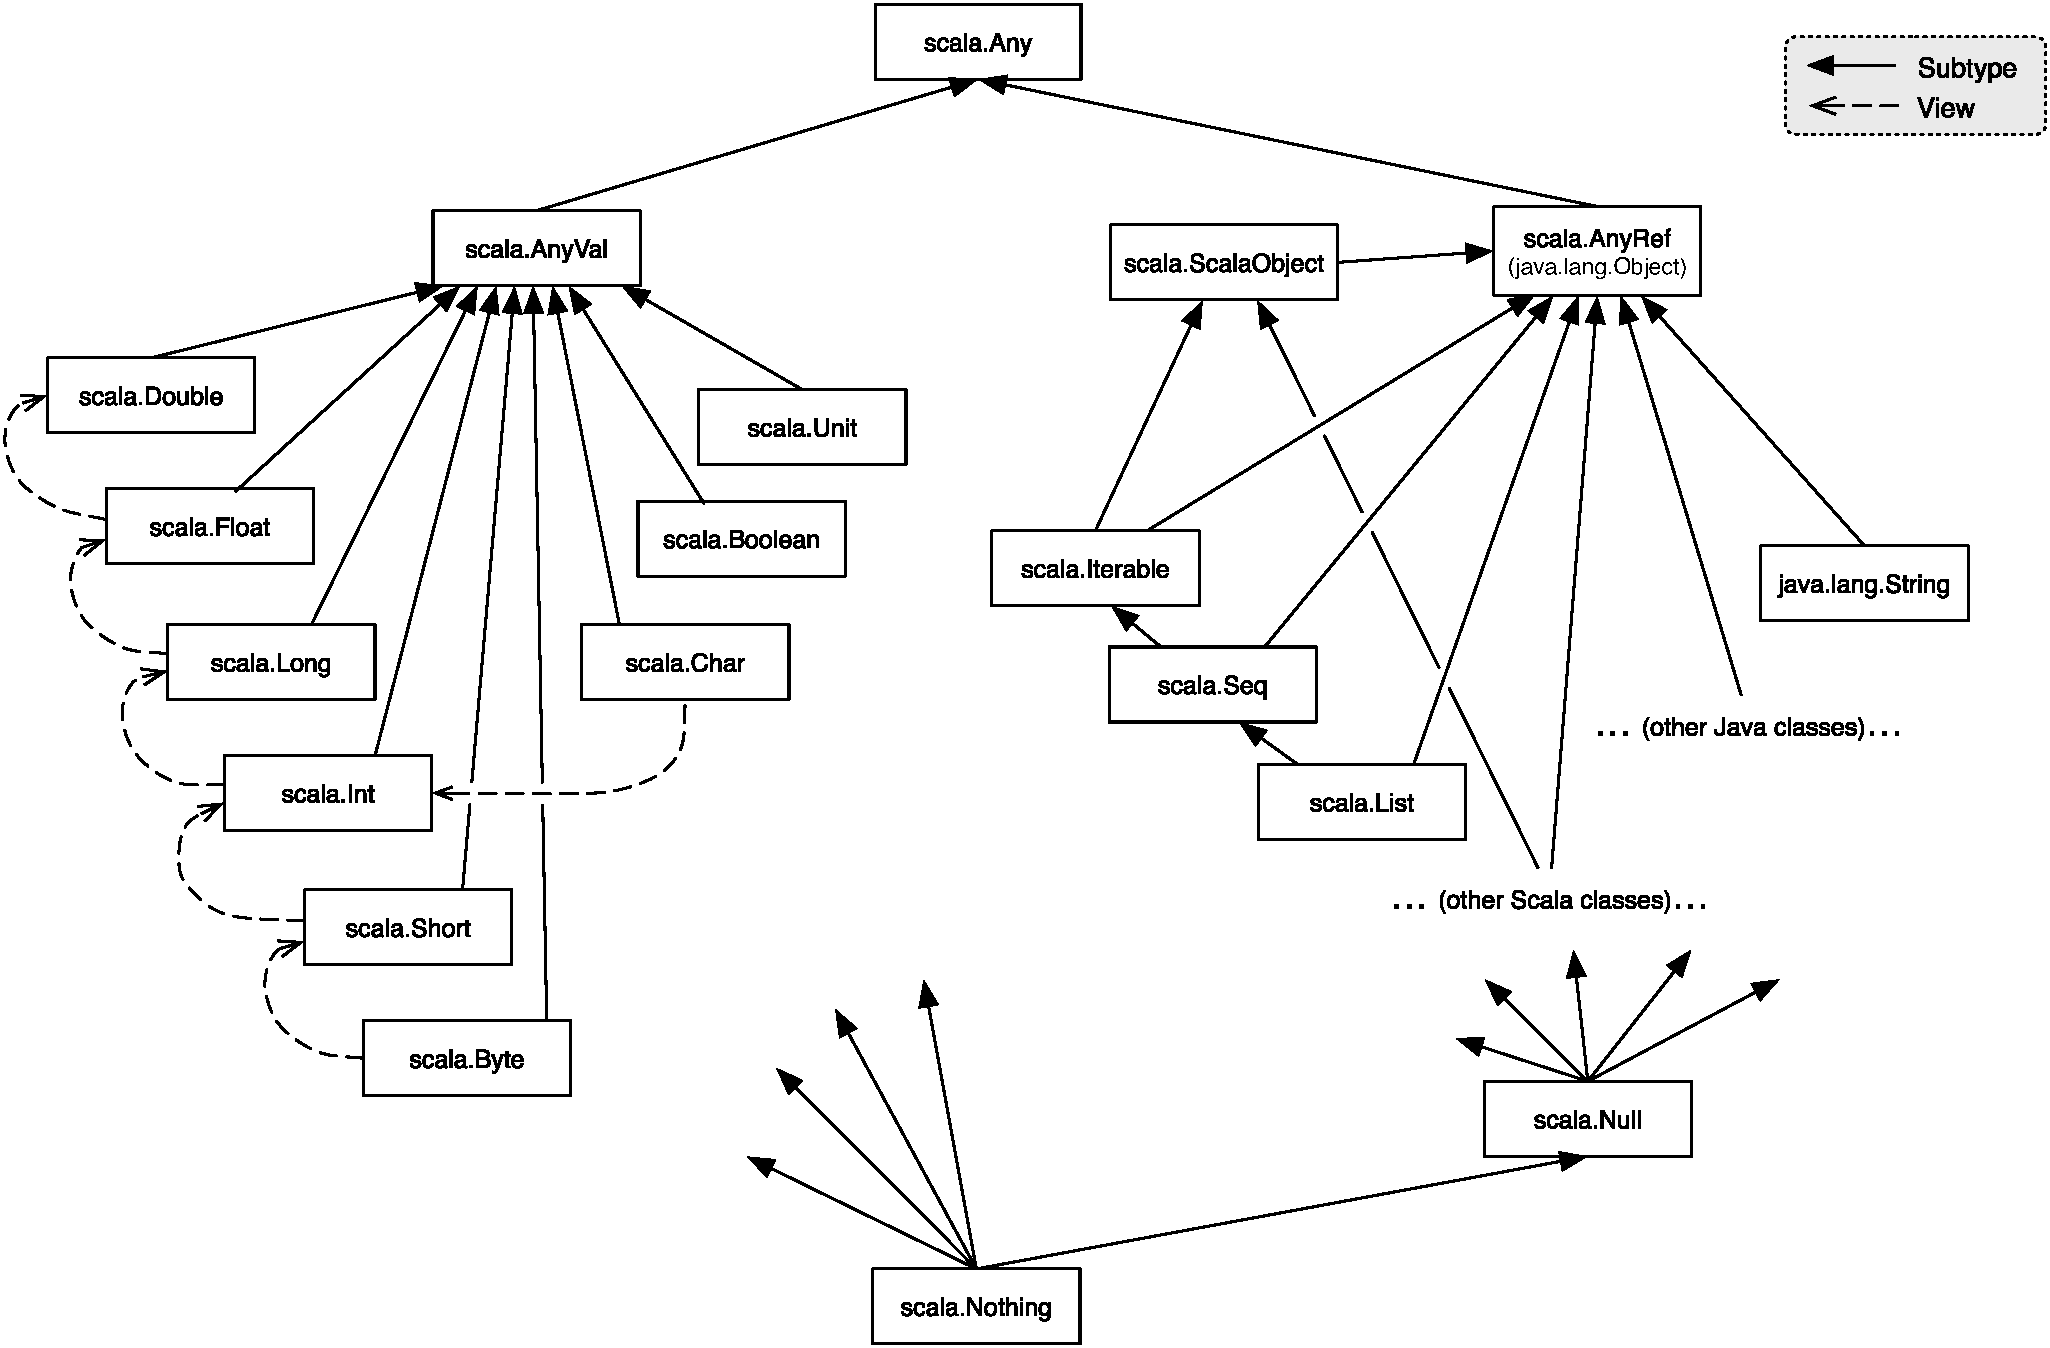
\includegraphics[scale=0.40]{classhierarchy}
\vspace*{-1.5mm}
\caption{Class hierarchy of Scala.}
\label{fig:class-hierarchy}
\end{figure*}

\section{Root Classes}
\label{sec:cls-root}
\label{sec:cls-any}
\label{sec:cls-object}

Figure~\ref{fig:class-hierarchy} illustrates Scala's class
hierarchy.
The root of this hierarchy is formed by class \code{Any}.
Every class in a Scala execution environment inherits directly or
indirectly from this class.  Class \code{Any} has two direct
subclasses: \code{AnyRef} and \code{AnyVal}.

The subclass \code{AnyRef} represents all values which are represented
as objects in the underlying host system. Every user-defined Scala
class inherits directly or indirectly from this class. Furthermore,
every user-defined Scala class also inherits the trait
\code{scala.ScalaObject}.  Classes written in other languages still
inherit from \code{scala.AnyRef}, but not from
\code{scala.ScalaObject}.

The class \code{AnyVal} has a fixed number of subclasses, which describe
values which are not implemented as objects in the underlying host
system.

Classes \code{AnyRef} and \code{AnyVal} are required to provide only
the members declared in class \code{Any}, but implementations may add
host-specific methods to these classes (for instance, an
implementation may identify class \code{AnyRef} with its own root
class for objects).

The signatures of these root classes are described by the following
definitions.

\begin{lstlisting}
package scala 
/** The universal root class */
abstract class Any {

  /** Defined equality; abstract here */
  def equals(that: Any): Boolean 

  /** Semantic equality between values */
  final def == (that: Any): Boolean  =  
    if (null eq this) null eq that else this equals that

  /** Semantic inequality between values */
  final def != (that: Any): Boolean  =  !(this == that)

  /** Hash code; abstract here */
  def hashCode: Int = $\ldots$

  /** Textual representation; abstract here */
  def toString: String = $\ldots$

  /** Type test; needs to be inlined to work as given */
  def isInstanceOf[a]: Boolean

  /** Type cast; needs to be inlined to work as given */ */
  def asInstanceOf[A]: A = this match {
    case x: A => x
    case _ => if (this eq null) this
              else throw new ClassCastException()
  }
}

/** The root class of all value types */
final class AnyVal extends Any 

/** The root class of all reference types */
class AnyRef extends Any {
  def equals(that: Any): Boolean      = this eq that 
  final def eq(that: AnyRef): Boolean = $\ldots$ // reference equality
  final def ne(that: AnyRef): Boolean = !(this eq that)

  def hashCode: Int = $\ldots$     // hashCode computed from allocation address
  def toString: String  = $\ldots$ // toString computed from hashCode and class name

  def synchronized[T](body: => T): T // execute `body` in while locking `this`.
}                           

/** A mixin class for every user-defined Scala class */
trait ScalaObject extends AnyRef 
\end{lstlisting}

The type test \lstinline@$x$.isInstanceOf[$T$]@ is equivalent to a typed
pattern match
\begin{lstlisting} 
$x$ match {
  case _: $T'$ => true
  case _ => false
}
\end{lstlisting} 
where the type $T'$ is the same as $T$ except if $T$ is
of the form $D$ or $D[\tps]$ where $D$ is a type member of some outer
class $C$. In this case $T'$ is \lstinline@$C$#$D$@ (or
\lstinline@$C$#$D[tps]$@, respectively), whereas $T$ itself would
expand to \lstinline@$C$.this.$D[tps]$@. In other words, an
\lstinline@isInstanceOf@ test does not check for the   


The test ~\lstinline@$x$.asInstanceOf[$T$]@ is treated specially if $T$ is a
numeric value type (\sref{sec:cls-value}). In this case the cast will
be translated to an application of a conversion method ~\lstinline@x.to$T$@ 
(\sref{cls:numeric-value}). For non-numeric values $x$ the operation will raise a
\code{ClassCastException}.

\section{Value Classes}
\label{sec:cls-value}

Value classes are classes whose instances are not represented as
objects by the underlying host system.  All value classes inherit from
class \code{AnyVal}. Scala implementations need to provide the
value classes \code{Unit}, \code{Boolean}, \code{Double}, \code{Float},
\code{Long}, \code{Int}, \code{Char}, \code{Short}, and \code{Byte}
(but are free to provide others as well).
The signatures of these classes are defined in the following.

\subsection{Numeric Value Types} \label{cls:numeric-value}

Classes \code{Double}, \code{Float},
\code{Long}, \code{Int}, \code{Char}, \code{Short}, and \code{Byte}
are together called {\em numeric value types}. Classes \code{Byte},
\code{Short}, or \code{Char} are called {\em subrange types}.
Subrange types, as well as \code{Int} and \code{Long} are called {\em
integer types}, whereas \code{Float} and \code{Double} are called {\em
floating point types}.

Numeric value types are ranked in the following partial order:

\begin{lstlisting}
Byte - Short 
             \
               Int - Long - Float - Double
             / 
        Char 
\end{lstlisting}
\code{Byte} and \code{Short} are the lowest-ranked types in this order, 
whereas \code{Double} is the highest-ranked.  Ranking does {\em not}
imply a conformance (\sref{sec:conformance}) relationship; for
instance \code{Int} is not a subtype of \code{Long}.  However, object
\code{Predef} (\sref{cls:predef}) defines views (\sref{sec:views}) 
from every numeric value type to all higher-ranked numeric value types. Therefore,
lower-ranked types are implicitly converted to higher-ranked types
when required by the context (\sref{sec:impl-conv}).

Given two numeric value types $S$ and $T$, the {\em operation type} of
$S$ and $T$ is defined as follows: If both $S$ and $T$ are subrange
types then the operation type of $S$ and $T$ is \code{Int}.  Otherwise
the operation type of $S$ and $T$ is the larger of the two types wrt
ranking. Given two numeric values $v$ and $w$ the operation type of
$v$ and $w$ is the operation type of their run-time types.

Any numeric value type $T$ supports the following methods.
\begin{itemize}
\item 
Comparison methods for equals (\code{==}), not-equals (\code{!=}),
less-than (\code{<}), greater-than (\code{>}), less-than-or-equals
(\code{<=}), greater-than-or-equals (\code{>=}), which each exist in 7
overloaded alternatives. Each alternative takes a parameter of some
numeric value type. Its result type is type \code{Boolean}. The
operation is evaluated by converting the receiver and its argument to
their operation type and performing the given comparison operation of
that type.
\item
Arithmetic methods addition (\code{+}), subtraction (\code{-}),
multiplication (\code{*}), division (\code{/}), and remainder
(\lstinline@%@), which each exist in 7 overloaded alternatives. Each
alternative takes a parameter of some numeric value type $U$.  Its
result type is the operation type of $T$ and $U$. The operation is
evaluated by converting the receiver and its argument to their
operation type and performing the given arithmetic operation of that
type.
\item
Parameterless arithmethic methods identity (\code{+}) and negation
(\code{-}), with result type $T$.  The first of these returns the
receiver unchanged, whereas the second returns its negation.
\item
Conversion methods \code{toByte}, \code{toShort}, \code{toChar},
\code{toInt}, \code{toLong}, \code{toFloat}, \code{toDouble} which
convert the receiver object to the target type, using the rules of
Java's numeric type cast operation. The conversion might truncate the
numeric value (as when going from \code{Long} to \code{Int} or from
\code{Int} to \code{Byte}) or it might lose precision (as when going
from \code{Double} to \code{Float} or when converting between
\code{Long} and \code{Float}). 
\end{itemize}

Integer numeric value types support in addition the following operations:
\begin{itemize}
\item 
Bit manipulation methods bitwise-and (\code{&}), bitwise-or
{\code{|}}, and bitwise-exclusive-or (\code{^}), which each exist in 5
overloaded alternatives. Each alternative takes a parameter of some
integer numeric value type. Its result type is the operation type of
$T$ and $U$. The operation is evaluated by converting the receiver and
its argument to their operation type and performing the given bitwise
operation of that type.
\item
A parameterless bit-negation method (\lstinline@~@). Its result type is
the reciver type $T$ or \code{Int}, whichever is larger.
The operation is evaluated by converting the receiver to the result
type and negating every bit in its value.
\item
Bit-shift methods left-shift (\code{<<}), arithmetic right-shift
(\code{>>}), and unsigned right-shift (\code{>>>}). Each of these
methods has two overloaded alternatives, which take a parameter $n$
of type \code{Int}, respectively \code{Long}. The result type of the
operation is the receiver type $T$, or \code{Int}, whichever is larger.
The operation is evaluated by converting the receiver to the result
type and performing the specified shift by $n$ bits.
\end{itemize}

Numeric value types also implement operations \code{equals},
\code{hashCode}, and \code{toString} from class \code{Any}.

The \code{equals} method tests whether the argument is a numeric value
type. If this is true, it will perform the \code{==} operation which
is appropriate for that type. That is, the \code{equals} method of a
numeric value type can be thought of being defined as follows:
\begin{lstlisting}
def equals(other: Any): Boolean = other match {
  case that: Byte   => this == that
  case that: Short  => this == that
  case that: Char   => this == that
  case that: Int    => this == that
  case that: Long   => this == that
  case that: Float  => this == that
  case that: Double => this == that
  case _ => false
}
\end{lstlisting}
The \code{hashCode} method returns an integer hashcode that maps equal
numeric values to equal results. It is guaranteed to be the identity for 
for type \code{Int} and for all subrange types.

The \code{toString} method displays its receiver as an integer or
floating point number.

\example As an example, here is the signature of the numeric value type \code{Int}:

\begin{lstlisting}
package scala 
abstract sealed class Int extends AnyVal {
  def == (that: Double): Boolean  // double equality
  def == (that: Float): Boolean   // float equality
  def == (that: Long): Boolean    // long equality
  def == (that: Int): Boolean     // int equality
  def == (that: Short): Boolean   // int equality
  def == (that: Byte): Boolean    // int equality
  def == (that: Char): Boolean    // int equality
  /* analogous for !=, <, >, <=, >= */

  def + (that: Double): Double    // double addition
  def + (that: Float): Double     // float addition
  def + (that: Long): Long        // long addition
  def + (that: Int): Int          // int addition
  def + (that: Short): Int        // int addition
  def + (that: Byte): Int         // int addition
  def + (that: Char): Int         // int addition
  /* analogous for -, *, /, % */
  
  def & (that: Long): Long        // long bitwise and
  def & (that: Int): Int          // int bitwise and
  def & (that: Short): Int        // int bitwise and
  def & (that: Byte): Int         // int bitwise and
  def & (that: Char): Int         // int bitwise and
  /* analogous for |, ^ */

  def << (cnt: Int): Int          // int left shift
  def << (cnt: Long): Int         // long left shift
  /* analogous for >>, >>> */

  def unary_+ : Int               // int identity
  def unary_- : Int               // int negation
  def unary_~ : Int               // int bitwise negation

  def toByte: Byte                // convert to Byte
  def toShort: Short              // convert to Short
  def toChar: Char                // convert to Char
  def toInt: Int                  // convert to Int
  def toLong: Long                // convert to Long
  def toFloat: Float              // convert to Float
  def toDouble: Double            // convert to Double
}
\end{lstlisting}

\subsection{Class \large{\code{Boolean}}}
\label{sec:cls-boolean}

Class \code{Boolean} has only two values: \code{true} and
\code{false}. It implements operations as given in the following
class definition.
\begin{lstlisting}
package scala 
abstract sealed class Boolean extends AnyVal {
  def && (p: => Boolean): Boolean = // boolean and
    if (this) p else false
  def || (p: => Boolean): Boolean = // boolean or
    if (this) true else p
  def &  (x: Boolean): Boolean =    // boolean strict and
    if (this) x else false
  def |  (x: Boolean): Boolean =    // boolean strict or
    if (this) true else x
  def == (x: Boolean): Boolean =    // boolean equality
    if (this) x else x.unary_!
  def != (x: Boolean): Boolean      // boolean inequality
    if (this) x.unary_! else x
  def unary_!: Boolean              // boolean negation
    if (this) false else true
}
\end{lstlisting}
The class also implements operations \code{equals}, \code{hashCode},
and \code{toString} from class \code{Any}.

The \code{equals} method returns \code{true} if the argument is the
same boolean value as the receiver, \code{false} otherwise.  The
\code{hashCode} method returns a fixed, implementation-specific hash-code when invoked on \code{true}, 
and a different, fixed, implementation-specific hash-code when invoked on \code{false}. The \code{toString} method
returns the receiver converted to a string, i.e.\ either \code{"true"}
or \code{"false"}.

\subsection{Class \large{\code{Unit}}}

Class \code{Unit} has only one value: \code{()}. It implements only
the three methods \code{equals}, \code{hashCode}, and \code{toString}
from class \code{Any}.

The \code{equals} method returns \code{true} if the argument is the
unit value \lstinline@()@, \code{false} otherwise.  The
\code{hashCode} method returns a fixed, implementation-specific hash-code, 
The \code{toString} method returns \code{"()"}.

\section{Standard Reference Classes}
\label{cls:reference}

This section presents some standard Scala reference classes which are
treated in a special way in Scala compiler -- either Scala provides
syntactic sugar for them, or the Scala compiler generates special code
for their operations. Other classes in the standard Scala library are
documented in the Scala library documentation by HTML pages.

\subsection{Class \large{\code{String}}}

Scala's \lstinline@String@ class is usually derived from the standard String
class of the underlying host system (and may be identified with
it). For Scala clients the class is taken to support in each case a
method
\begin{lstlisting}
def + (that: Any): String 
\end{lstlisting}
which concatenates its left operand with the textual representation of its
right operand.

\subsection{The \large{\code{Tuple}} classes}

Scala defines tuple classes \lstinline@Tuple$n$@ for $n = 2 \commadots 22$.
These are defined as follows.

\begin{lstlisting}
package scala 
case class Tuple$n$[+T_1, ..., +T_n](_1: T_1, ..., _$n$: T_$n$) {
  def toString = "(" ++ _1 ++ "," ++ $\ldots$ ++ "," ++ _$n$ ++ ")"
}
\end{lstlisting}

The implicitly imported \code{Predef} object (\sref{cls:predef}) defines
the names \code{Pair} as an alias of \code{Tuple2} and \code{Triple}
as an alias for \code{Tuple3}.

\subsection{The \large{\code{Function}} Classes}
\label{sec:cls-function}

Scala defines function classes \lstinline@Function$n$@ for $n = 1 \commadots 22$.
These are defined as follows.

\begin{lstlisting}
package scala 
trait Function$n$[-T_1, ..., -T_$n$, +R] {
  def apply(x_1: T_1, ..., x_$n$: T_$n$): R
  def toString = "<function>" 
}
\end{lstlisting}

\comment{
There is also a module \code{Function}, which provides additional utility methods
regarding currying and tupling.
}
A subclass of \lstinline@Function1@ represents partial functions,
which are undefined on some points in their domain. In addition to the
\code{apply} method of functions, partial functions also have a
\code{isDefined} method, which tells whether the function is defined
at the given argument:
\begin{lstlisting}
class PartialFunction[-A, +B] extends Function1[A, B] {
  def isDefinedAt(x: A): Boolean
}
\end{lstlisting}

The implicitly imported \code{Predef} object (\sref{cls:predef}) defines the name 
\code{Function} as an alias of \code{Function1}.

\subsection{Class \large{\code{Array}}}\label{cls:array}

The class of generic arrays is given as follows.

\begin{lstlisting}
final class Array[A](len: Int) extends Seq[A] {
  def length: Int = len
  def apply(i: Int): A = $\ldots$
  def update(i: Int, x: A): Unit = $\ldots$
  def elements: Iterator[A] = $\ldots$
  def subArray(from: Int, end: Int): Array[A] = $\ldots$
  def filter(p: A => Boolean): Array[A] = $\ldots$
  def map[B](f: A => B): Array[B] = $\ldots$
  def flatMap[B](f: A => Array[B]): Array[B] = $\ldots$
}
\end{lstlisting}
If $T$ is not a type parameter or abstract type, the type Array[$T$]
is represented as the native array type \lstinline{[]$T$} in the
underlying host system. In that case \code{length} returns
the length of the array, \code{apply} means subscripting, and
\code{update} means element update. Because of the syntactic sugar for
\code{apply} and
%\code{update} operations (\sref{sec:impl-conv}, \sref{sec:assignments}),
\code{update} operations (\sref{sec:impl-conv},
we have the following correspondences between Scala and Java/C\# code for
operations on an array \code{xs}:

\begin{lstlisting}
$\mbox{\em Scala}$            $\mbox{\em Java/C\#}$
  xs.length        xs.length
  xs(i)            xs[i]
  xs(i) = e        xs[i] = e
\end{lstlisting}

Arrays also implement the sequence trait \code{scala.Seq}
by defining an \code{elements} method which returns
all elements of the array in an \code{Iterator}.

Because of the tension between parametrized types in Scala and the ad-hoc
implementation of arrays in the host-languages, some subtle points
need to be taken into account when dealing with arrays. These are
explained in the following.

First, unlike arrays in Java or C\#, arrays in Scala are {\em not}
co-variant; That is, $S <: T$ does not imply 
~\lstinline@Array[$S$] $<:$ Array[$T$]@ in Scala.  
However, it is possible to cast an array
of $S$ to an array of $T$ if such a cast is permitted in the host
environment.

For instance \code{Array[String]} does not conform to
\code{Array[Object]}, even though \code{String} conforms to \code{Object}.
However, it is possible to cast an expression of type
~\lstinline@Array[String]@~ to ~\lstinline@Array[Object]@, and this
cast will succeed without raising a \code{ClassCastException}. Example:
\begin{lstlisting}
val xs = new Array[String](2)
// val ys: Array[Object] = xs   // **** error: incompatible types
val ys: Array[Object] = xs.asInstanceOf[Array[Object]] // OK
\end{lstlisting}

Second, for {\em polymorphic arrays}, that have a type parameter or
abstract type $T$ as their element type, a representation different
from
\lstinline@[]T@ might be used. However, it is guaranteed that 
\code{isInstanceOf} and \code{asInstanceOf} still work as if the array 
used the standard representation of monomorphic arrays:
\begin{lstlisting}
val ss = new Array[String](2)

def f[T](xs: Array[T]): Array[String] = 
  if (xs.isInstanceOf[Array[String]]) xs.asInstanceOf[Array[String])
  else throw new Error("not an instance")

f(ss)                                     // returns ss
\end{lstlisting}
The representation chosen for polymorphic arrays also guarantees that
polymorphic array creations work as expected. An example is the
following implementation of method \lstinline@mkArray@, which creates
an array of an arbitrary type $T$, given a sequence of $T$'s which
defines its elements.
\begin{lstlisting}
def mkArray[T](elems: Seq[T]): Array[T] = {
  val result = new Array[T](elems.length)
  var i = 0
  for (elem <- elems) {
    result(i) = elem
    i += 1
  }
}
\end{lstlisting}
Note that under Java's erasure model of arrays the method above would
not work as expected -- in fact it would always return an array of
\lstinline@Object@.

Third, in a Java environment there is a method \code{System.arraycopy}
which takes two objects as parameters together with start indices and
a length argument, and copies elements from one object to the other,
provided the objects are arrays of compatible element
types. \code{System.arraycopy} will not work for Scala's polymorphic
arrays because of their different representation. One should instead
use method \code{Array.copy} which is defined in the companion object
of class \lstinline@Array@. This companion object also defines various
constructor methods for arrays, as well as 
the extractor method \code{unapplySeq} (\sref{sec:extractor-patterns})
which enables pattern matching over arrays.
\begin{lstlisting}
package scala
object Array { 
  /** copies array elements from `src' to `dest'. */
  def copy(src: AnyRef, srcPos: Int, 
           dest: AnyRef, destPos: Int, length: Int): Unit = $\ldots$

  /** Concatenate all argument arrays into a single array. */
  def concat[T](xs: Array[T]*): Array[T] = $\ldots$

  /** Create a an array of successive integers. */
  def range(start: Int, end: Int): Array[Int] = $\ldots$

  /** Create an array with given elements. */
  def apply[A <: AnyRef](xs: A*): Array[A] = $\ldots$

  /** Analogous to above. */
  def apply(xs: Boolean*): Array[Boolean] = $\ldots$
  def apply(xs: Byte*)   : Array[Byte]    = $\ldots$
  def apply(xs: Short*)  : Array[Short]   = $\ldots$
  def apply(xs: Char*)   : Array[Char]    = $\ldots$
  def apply(xs: Int*)    : Array[Int]     = $\ldots$
  def apply(xs: Long*)   : Array[Long]    = $\ldots$
  def apply(xs: Float*)  : Array[Float]   = $\ldots$
  def apply(xs: Double*) : Array[Double]  = $\ldots$
  def apply(xs: Unit*)   : Array[Unit]    = $\ldots$

  /** Create an array containing several copies of an element. */
  def make[A](n: Int, elem: A): Array[A] = {

  /** Enables pattern matching over arrays */
  def unapplySeq[A](x: Array[A]): Option[Seq[A]] = Some(x)
}
\end{lstlisting}

\example The following method duplicates a given argument array and returns a pair consisting of the original and the duplicate:
\begin{lstlisting}
def duplicate[T](xs: Array[T]) = {
  val ys = new Array[T](xs.length)
  Array.copy(xs, 0, ys, 0, xs.length)
  (xs, ys)
}
\end{lstlisting}

\section{Class Node}\label{cls:Node}
\begin{lstlisting}
package scala.xml 

trait Node {

  /** the label of this node */
  def label: String               

  /** attribute axis */
  def attribute: Map[String, String] 

  /** child axis (all children of this node) */
  def child: Seq[Node]          

  /** descendant axis (all descendants of this node) */
  def descendant: Seq[Node] = child.toList.flatMap { 
    x => x::x.descendant.asInstanceOf[List[Node]] 
  } 

  /** descendant axis (all descendants of this node) */
  def descendant_or_self: Seq[Node] = this::child.toList.flatMap { 
    x => x::x.descendant.asInstanceOf[List[Node]] 
  } 

  override def equals(x: Any): Boolean = x match {
    case that:Node => 
      that.label == this.label && 
        that.attribute.sameElements(this.attribute) && 
          that.child.sameElements(this.child)
    case _ => false
  } 

 /** XPath style projection function. Returns all children of this node
  *  that are labeled with 'that'. The document order is preserved.
  */
    def \(that: Symbol): NodeSeq = {
      new NodeSeq({
        that.name match {
          case "_" => child.toList  
          case _ =>
            var res:List[Node] = Nil 
            for (x <- child.elements if x.label == that.name) {
              res = x::res 
            }
            res.reverse
        }
      }) 
    }

 /** XPath style projection function. Returns all nodes labeled with the 
  *  name 'that' from the 'descendant_or_self' axis. Document order is preserved.
  */
  def \\(that: Symbol): NodeSeq = {
    new NodeSeq(
      that.name match {
        case "_" => this.descendant_or_self 
        case _ => this.descendant_or_self.asInstanceOf[List[Node]].
        filter(x => x.label == that.name) 
      })
  }

  /** hashcode for this XML node */
  override def hashCode = 
    Utility.hashCode(label, attribute.toList.hashCode, child) 

  /** string representation of this node */
  override def toString = Utility.toXML(this) 

}
\end{lstlisting}

\newpage
\section{The \large{\code{Predef}} Object}\label{cls:predef}

The \code{Predef} object defines standard functions and type aliases
for Scala programs. It is always implicitly imported, so that all its
defined members are available without qualification. Its definition
for the JVM environment conforms to the following signature:

\begin{lstlisting}
package scala
object Predef {

  // classOf ---------------------------------------------------------

  /** Returns the runtime representation of a class type. */
  def classOf[T]: Class[T] = null  
   // this is a dummy, classOf is handled by compiler.

  // Standard type aliases ---------------------------------------------

  type String    = java.lang.String
  type Class[T]  = java.lang.Class[T]

  // Miscellaneous -----------------------------------------------------
  
  type Function[-A, +B] = Function1[A, B]

  type Map[A, +B] = collection.immutable.Map[A, B]
  type Set[A] = collection.immutable.Set[A]

  val Map = collection.immutable.Map
  val Set = collection.immutable.Set

  // Manifest types, companions, and incantations for summoning ---------

  type ClassManifest[T] = scala.reflect.ClassManifest[T]
  type Manifest[T]      = scala.reflect.Manifest[T]
  type OptManifest[T]   = scala.reflect.OptManifest[T]
  val ClassManifest     = scala.reflect.ClassManifest
  val Manifest          = scala.reflect.Manifest
  val NoManifest        = scala.reflect.NoManifest
  
  def manifest[T](implicit m: Manifest[T])           = m
  def classManifest[T](implicit m: ClassManifest[T]) = m
  def optManifest[T](implicit m: OptManifest[T])     = m

  // Minor variations on identity functions -----------------------------
  def identity[A](x: A): A         = x    // @see `conforms` for the implicit version
  def implicitly[T](implicit e: T) = e    // for summoning implicit values from the nether world
  @inline def locally[T](x: T): T  = x    // to communicate intent and avoid unmoored statements

  // Asserts, Preconditions, Postconditions -----------------------------

  def assert(assertion: Boolean) {
    if (!assertion)
      throw new java.lang.AssertionError("assertion failed")
  }

  def assert(assertion: Boolean, message: => Any) {
    if (!assertion)
      throw new java.lang.AssertionError("assertion failed: " + message)
  }

  def assume(assumption: Boolean) {
    if (!assumption)
      throw new IllegalArgumentException("assumption failed")
  }

  def assume(assumption: Boolean, message: => Any) {
    if (!assumption)
      throw new IllegalArgumentException(message.toString)
  }

  def require(requirement: Boolean) {
    if (!requirement)
      throw new IllegalArgumentException("requirement failed")
  }

  def require(requirement: Boolean, message: => Any) {
    if (!requirement)
      throw new IllegalArgumentException("requirement failed: "+ message)
  }
  \end{lstlisting}
\newpage
\begin{lstlisting}

  // tupling ---------------------------------------------------------

  type Pair[+A, +B] = Tuple2[A, B]
  object Pair {
    def apply[A, B](x: A, y: B) = Tuple2(x, y)
    def unapply[A, B](x: Tuple2[A, B]): Option[Tuple2[A, B]] = Some(x)
  }

  type Triple[+A, +B, +C] = Tuple3[A, B, C]
  object Triple {
    def apply[A, B, C](x: A, y: B, z: C) = Tuple3(x, y, z)
    def unapply[A, B, C](x: Tuple3[A, B, C]): Option[Tuple3[A, B, C]] = Some(x)
  }

  // Printing and reading -----------------------------------------------

  def print(x: Any) = Console.print(x)
  def println() = Console.println()
  def println(x: Any) = Console.println(x)
  def printf(text: String, xs: Any*) = Console.printf(text.format(xs: _*))

  def readLine(): String = Console.readLine()
  def readLine(text: String, args: Any*) = Console.readLine(text, args)
  def readBoolean() = Console.readBoolean()
  def readByte() = Console.readByte()
  def readShort() = Console.readShort()
  def readChar() = Console.readChar()
  def readInt() = Console.readInt()
  def readLong() = Console.readLong()
  def readFloat() = Console.readFloat()
  def readDouble() = Console.readDouble()
  def readf(format: String) = Console.readf(format)
  def readf1(format: String) = Console.readf1(format)
  def readf2(format: String) = Console.readf2(format)
  def readf3(format: String) = Console.readf3(format)

  // Implict conversions ------------------------------------------------

  ...
}
\end{lstlisting}

\subsection{Predefined Implicit Definitions}

The \lstinline@Predef@ object also contains a number of implicit definitions, which are available by default (because \lstinline@Predef@ is implicitly imported).
Implicit definitions come in two priorities. High-priority implicits are defined in the \lstinline@Predef@ class itself whereas low priority implicits are defined in a class inherited by \lstinline@Predef@. The rules of 
static overloading resolution (\sref{sec:overloading-resolution})
stipulate that, all other things being equal, implicit resolution 
prefers high-priority implicits over low-priority ones.

The available low-priority implicits include definitions falling into the following categories.

\begin{enumerate}
\item
For every primitive type, a wrapper that takes values of that type
to instances of a \lstinline@runtime.Rich*@ class. For instance, values of type \lstinline@Int@
can be implicitly converted to instances of class \lstinline@runtime.RichInt@.
\item
For every array type with elements of primitive type, a wrapper that
takes the arrays of that type to instances of a \lstinline@runtime.WrappedArray@ class. For instance, values of type \lstinline@Array[Float]@ can be implicitly converted to instances of class \lstinline@runtime.WrappedArray[Float]@.
There are also generic array wrappers that take elements
of type \lstinline@Array[T]@ for arbitrary \lstinline@T@ to \lstinline@WrappedArray@s.
\item
An implicit conversion from \lstinline@String@ to \lstinline@WrappedString@.
\end{enumerate}

The available high-priority implicits include definitions falling into the following categories.

\begin{itemize}
\item
An implicit wrapper that adds \lstinline@ensuring@ methods 
with the following overloaded variants to type \lstinline@Any@.
\begin{lstlisting}
    def ensuring(cond: Boolean): A = { assert(cond); x }
    def ensuring(cond: Boolean, msg: Any): A = { assert(cond, msg); x }
    def ensuring(cond: A => Boolean): A = { assert(cond(x)); x }
    def ensuring(cond: A => Boolean, msg: Any): A = { assert(cond(x), msg); x }
\end{lstlisting}
\item
An implicit wrapper that adds a \lstinline@->@ method with the following implementation
to type \lstinline@Any@.
\begin{lstlisting}
    def -> [B](y: B): (A, B) = (x, y)
\end{lstlisting}
\item
For every array type with elements of primitive type, a wrapper that
takes the arrays of that type to instances of a \lstinline@runtime.ArrayOps@
class. For instance, values of type \lstinline@Array[Float]@ can be implicitly
converted to instances of class \lstinline@runtime.ArrayOps[Float]@.  There are
also generic array wrappers that take elements of type \lstinline@Array[T]@ for
arbitrary \lstinline@T@ to \lstinline@ArrayOps@s.
\item
An implicit wrapper that adds \lstinline@+@ and \lstinline@formatted@ method with the following implementations
to type \lstinline@Any@.
\begin{lstlisting}
  def +(other: String) = String.valueOf(self) + other
  def formatted(fmtstr: String): String = fmtstr format self
\end{lstlisting}
\item
Numeric primitive conversions that implement the transitive closure of the following
mappings:

\begin{minipage}{\linewidth}
\begin{lstlisting}
  Byte  -> Short
  Short -> Int
  Char  -> Int
  Int   -> Long
  Long  -> Float
  Float -> Double
\end{lstlisting}
\end{minipage}

\item
Boxing and unboxing conversions between primitive types and their boxed versions:
\begin{lstlisting}
  Byte    <-> java.lang.Byte
  Short   <-> java.lang.Short
  Char    <-> java.lang.Character
  Int     <-> java.lang.Integer
  Long    <-> java.lang.Long
  Float   <-> java.lang.Float
  Double  <-> java.lang.Double
  Boolean <-> java.lang.Boolean
\end{lstlisting}
\item
An implicit definition that generates instances of type \lstinline@T <:< T@, for
any type \lstinline@T@. Here, \lstinline@<:<@ is a class defined as follows.
\begin{lstlisting}
  sealed abstract class <:<[-From, +To] extends (From => To)
\end{lstlisting}
Implicit parameters of \lstinline@<:<@ types are typically used to implement type constraints.
\end{itemize}


\comment{
\subsection{Base Classes}
\label{sec:base-classes}

For every template, class type and constructor invocation we define
two sets of class types: the {\em base classes} and {\em mixin base
classes}. Their definitions are as follows.

The {\em mixin base classes} of a template 
~\lstinline@$sc$ with $mt_1$ with $\ldots$ with $mt_n$ {$\stats\,$}@~ 
are 
the reduced union (\sref{sec:base-classes-member-defs}) of the base classes of all
mixins $mt_i$. The mixin base classes of a class type $C$ are the
mixin base classes of the template augmented by $C$ itself. The
mixin base classes of a constructor invocation of type $T$ are the
mixin base classes of class $T$.

The {\em base classes} of a template consist are the reduced union of
the base classes of its superclass and the template's mixin base
classes.  The base classes of class \lstinline@scala.Any@ consist of
just the class itself. The base classes of some other class type $C$
are the base classes of the template represented by $C$ augmented by
$C$ itself.  The base classes of a constructor invocation of type $T$
are the base classes of $T$.

The notions of mixin base classes and base classes are extended from
classes to arbitrary types following the definitions of
\sref{sec:base-classes-member-defs}.

\comment{
If two types in the base class sequence of a template refer to the
same class definition, then that definition must define a trait
(\sref{sec:traits}), and the type that comes later in the sequence must
conform to the type that comes first. 
(\sref{sec:base-classes-member-defs}).
}

\example 
Consider the following class definitions:
\begin{lstlisting}
class A 
class B extends A 
trait C extends A 
class D extends A 
class E extends B with C with D 
class F extends B with D with E 
\end{lstlisting} 
The mixin base classes and base classes of classes \code{A-F} are given in
the following table:
\begin{quote}\begin{tabular}{|l|l|l|} \hline
 \ & Mixin base classes & Base classes \\  \hline
A & A & A, ScalaObject, AnyRef, Any \\
B & B & B, A, ScalaObject, AnyRef, Any \\
C & C & C, A, ScalaObject, AnyRef, Any \\
D & D & D, A, ScalaObject, AnyRef, Any \\
E & C, D, E & E, B, C, D, A, ScalaObject, AnyRef, Any \\
F & C, D, E, F & F, B, D, E, C, A, ScalaObject, AnyRef, Any \\ \hline
\end{tabular}\end{quote}
Note that \code{D} is inherited twice by \code{F}, once directly, the
other time indirectly through \code{E}. This is permitted, since
\code{D} is a trait.
}
